\documentclass[10pt,a4paper]{article}
\usepackage[T1]{fontenc}
\usepackage[utf8]{inputenc}
\usepackage{lmodern}
\usepackage[a4paper,margin=24mm]{geometry}
\usepackage{microtype}
\usepackage{booktabs}
\usepackage{tabularx}
\usepackage{array}
\usepackage{enumitem}
\usepackage{xcolor}
\usepackage{caption}
\usepackage{titlesec}
\usepackage{fancyhdr}
\usepackage[section]{placeins}
\usepackage{float}
\usepackage{xurl}
\usepackage{tikz}
\usetikzlibrary{arrows.meta,positioning,calc,fit}
\usepackage[hidelinks]{hyperref}

\definecolor{ink}{HTML}{1F2933}
\definecolor{accent}{HTML}{1D5C8A}
\definecolor{fillA}{HTML}{E6EEF5}
\definecolor{fillB}{HTML}{F3EDE2}
\definecolor{fillC}{HTML}{E8F1E6}
\definecolor{fillD}{HTML}{F0F0F0}
\color{ink}

\setlist{itemsep=1pt,topsep=3pt,leftmargin=1.4em}
\setlength{\parindent}{0pt}
\setlength{\parskip}{5pt}
\captionsetup{font=small,labelfont=bf,skip=6pt}
\titleformat{\section}{\large\bfseries\color{accent}}{\thesection}{0.7em}{}
\titleformat{\subsection}{\normalsize\bfseries}{\thesubsection}{0.7em}{}
\titlespacing*{\section}{0pt}{14pt}{4pt}
\titlespacing*{\subsection}{0pt}{9pt}{2pt}
\pagestyle{fancy}
\fancyhf{}
\renewcommand{\headrulewidth}{0.3pt}
\fancyhead[L]{\small rcore8 protocol emulator: datasheet}
\fancyhead[R]{\small Preliminary, revision 0.3}
\fancyfoot[C]{\small\thepage}
\newcolumntype{L}{>{\raggedright\arraybackslash}X}
\newcommand{\est}{\textsuperscript{e}}
\newcommand{\reg}[1]{\texttt{#1}}

\tikzset{
  blk/.style={draw=ink,line width=0.5pt,rounded corners=1.5pt,align=center,font=\small,inner sep=4pt,minimum height=8mm},
  ar/.style={-{Stealth[length=2mm]},line width=0.5pt},
  dar/.style={{Stealth[length=2mm]}-{Stealth[length=2mm]},line width=0.5pt},
  lbl/.style={font=\scriptsize,align=center}
}

\usepackage{longtable}
\usepackage{multicol}
\usepackage{colortbl}
\usepackage{listings}
\lstset{language=C,basicstyle=\ttfamily\footnotesize,keywordstyle=\color{accent}\bfseries,commentstyle=\color{black!55},
  columns=fullflexible,keepspaces=true,frame=single,rulecolor=\color{black!30},backgroundcolor=\color{black!3},
  breaklines=true,showstringspaces=false,xleftmargin=2pt,xrightmargin=2pt,aboveskip=6pt,belowskip=6pt,
  morekeywords={uint8_t,uint16_t,uint32_t}}
\newcommand{\tbd}{\textcolor{black!50}{\textit{TBD}}}
\begin{document}

\begin{center}
{\LARGE\bfseries\color{accent} rcore8 protocol emulator}\\[4pt]
{\large Two-core 8-bit RISC microcontroller with programmable line cells for serial protocols}\\[6pt]
{\large Preliminary datasheet}\\[8pt]
Tim S.\ B.\ (GitHub: cpldcpu)\\[2pt]
{\small Revision 0.3, 21 November 2026. Based on specification draft 0.36. Drafted with Claude (Anthropic).}
\end{center}

\noindent\fcolorbox{accent}{fillA}{\parbox{\dimexpr\linewidth-2\fboxsep-2\fboxrule}{\small
\textbf{Status of this document.} The device does not exist in silicon. All functional data are from RTL
simulation; rates and limits are given in clock cycles and converted with a 60\,MHz clock. Electrical data,
timing against real pins, the internal oscillator, package and ordering information are not available yet and
are marked \tbd. Values marked with a superscript e are estimates.}}

{\small\setcounter{tocdepth}{2}\begin{multicols}{2}\tableofcontents\end{multicols}}

\section{Features}

\begin{itemize}
\item \textbf{Two 8-bit RISC cores} with 16 registers and 70 instructions of 16 bit; most instructions take one
clock cycle. Programmed in C with GCC (section~\ref{sec:tools}).
\item \textbf{Memory:} 2\,KB of code memory per core (1\,024 words of 16 bit, SRAM), 2\,KB of shared data memory.
A program for one core can use both code memories (4\,KB).
\item \textbf{Program loaded by a host} through an SPI host link after reset; no non-volatile memory on the chip.
The host link also gives halt, single step, instruction injection, memory and register access, and a mailbox.
\item \textbf{Two pairs of line cells.} Each pair has a receive cell and a transmit cell that handle the bit level
of a serial protocol: timing, line code, bit stuffing, framing with parity or a ninth bit, start and stop conditions of a two-wire bus, clocked or self-timed operation. Configurations
exist for UART, SPI master and slave, I2C slave, WS2812 controller and LED, USB low-speed, 10BASE-T.
\item \textbf{8 bidirectional pins} for the line cells or as port pins, 8 input pins, 7 output pins.
\item \textbf{16-bit timer} with two compare values and capture from a pin or a line cell event; \textbf{three PWM
channels}; \textbf{CRC unit} with programmable polynomial up to 32 bit, fed by software or by a line cell.
\item \textbf{Event system:} 16 event flags per core, wait for a set of flags without polling, 16 interrupt
vectors, a shared time base with a wake-up time per core, four locks between the cores.
\item \textbf{Clocking:} external clock up to 60\,MHz\,(\tbd) or internal oscillator with 8-bit trim; trim counter
and loop against a reference pin, the host clock or a line event (USB keep-alive); separate dividers for
cores and peripherals.
\item \textbf{Program protection:} write enables and a lock for the code memories.
\item Technology: IHP 130\,nm CMOS with five metal layers, through Tiny Tapeout. Supply voltage, temperature range, package: \tbd.
\end{itemize}

\section{Description}

The device is a host-loaded microcontroller for emulating and bridging serial protocols. The bit-level work of a
protocol is done by the line cells, which are configured by registers and need no program. The cores move
bytes, keep protocol state and answer within the deadlines of the protocol. With two cores, one core can serve
a protocol with tight deadlines, for instance USB, while the other runs a second protocol or the application.

\begin{figure}[H]
\centering
\resizebox{0.92\textwidth}{!}{% SPDX-FileCopyrightText: (c) 2026 Tim S. B. (GitHub: cpldcpu)
% SPDX-License-Identifier: Apache-2.0
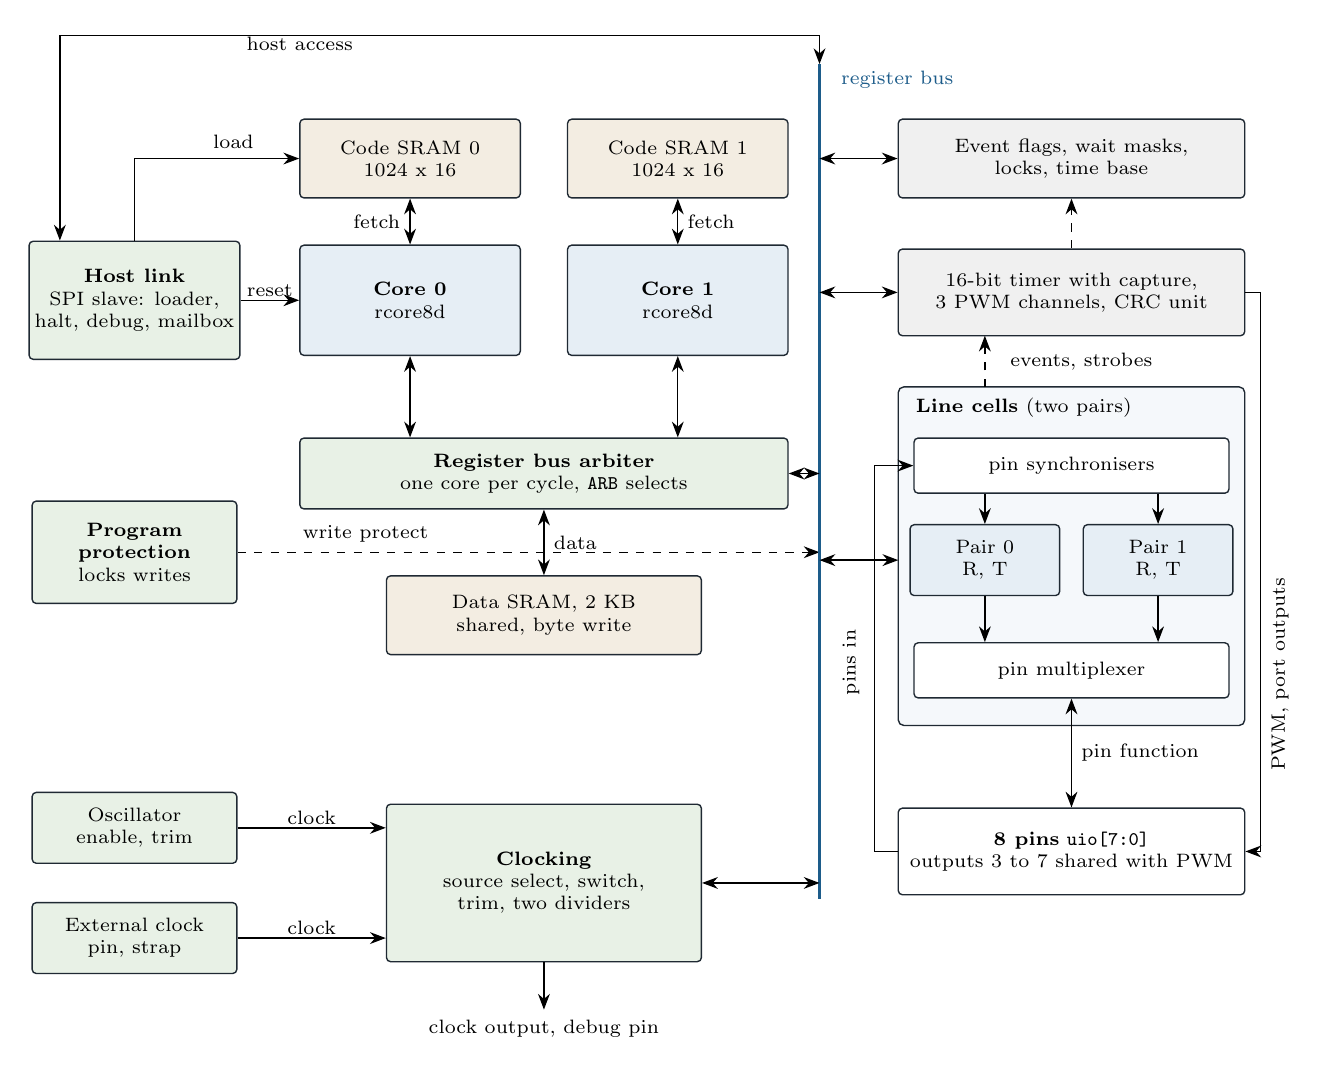
\begin{tikzpicture}[x=1mm,y=1mm,
  bk/.style={blk,font=\scriptsize,inner sep=2pt,align=center}]
  % host and protection
  \node[bk,fill=fillC,minimum width=26mm,minimum height=15mm] (host) at (17,94) {\textbf{Host link}\\ SPI slave: loader,\\ halt, debug, mailbox};
  \node[bk,fill=fillC,minimum width=26mm,minimum height=13mm] (prot) at (17,62) {\textbf{Program}\\ \textbf{protection}\\ locks writes};
  % memories and cores
  \node[bk,fill=fillB,minimum width=28mm,minimum height=10mm] (pm0) at (52,112) {Code SRAM 0\\ 1024 x 16};
  \node[bk,fill=fillB,minimum width=28mm,minimum height=10mm] (pm1) at (86,112) {Code SRAM 1\\ 1024 x 16};
  \node[bk,fill=fillA,minimum width=28mm,minimum height=14mm] (c0) at (52,94) {\textbf{Core 0}\\ rcore8d};
  \node[bk,fill=fillA,minimum width=28mm,minimum height=14mm] (c1) at (86,94) {\textbf{Core 1}\\ rcore8d};
  \node[bk,fill=fillC,minimum width=62mm,minimum height=9mm] (arb) at (69,72) {\textbf{Register bus arbiter}\\ one core per cycle, \reg{ARB} selects};
  \node[bk,fill=fillB,minimum width=40mm,minimum height=10mm] (dm) at (69,54) {Data SRAM, 2 KB\\ shared, byte write};
  \draw[dar] (pm0) -- (c0) node[midway,left,lbl]{fetch};
  \draw[dar] (pm1) -- (c1) node[midway,right,lbl]{fetch};
  \draw[dar] (c0.south) -- (c0.south |- arb.north);
  \draw[dar] (c1.south) -- (c1.south |- arb.north);
  \draw[dar] (arb) -- (dm) node[midway,right,lbl]{data};
  \draw[ar] (host.east) -- (c0.west) node[midway,above,lbl,inner sep=1pt]{reset};
  \draw[ar] (host.north) |- (pm0.west) node[pos=0.8,above,lbl]{load};
  \draw[ar,dashed] (prot.east) -- (104,62) node[pos=0.22,above,lbl]{write protect};
  % register bus
  \draw[line width=1.2pt,accent] (104,18) -- (104,124);
  \node[lbl,text=accent,anchor=west] at (105.5,122) {register bus};
  \draw[dar] (arb.east) -- (104,72);
  \draw[dar] (host.north west) ++(4,0) -- ++(0,26) -| (104,124);
  \node[lbl,anchor=south west] at (30,124.5) {host access};
  % right column
  \node[bk,fill=fillD,minimum width=44mm,minimum height=10mm] (ev) at (136,112) {Event flags, wait masks,\\ locks, time base};
  \node[bk,fill=fillD,minimum width=44mm,minimum height=11mm] (tm) at (136,95) {16-bit timer with capture,\\ 3 PWM channels, CRC unit};
  \draw[dar] (104,112) -- (ev.west);
  \draw[dar] (104,95) -- (tm.west);
  \draw[ar,dashed] (tm.north) -- (ev.south);
  % line cells
  \draw[blk,fill=fillA!40,rounded corners=2pt] (114,40) rectangle (158,83);
  \node[lbl,anchor=north west] at (115,82.8) {\textbf{Line cells} (two pairs)};
  \node[bk,fill=white,minimum width=40mm,minimum height=7mm] (sy) at (136,73) {pin synchronisers};
  \node[bk,fill=fillA,minimum width=19mm,minimum height=9mm] (p0) at (125,61) {Pair 0\\ R, T};
  \node[bk,fill=fillA,minimum width=19mm,minimum height=9mm] (p1) at (147,61) {Pair 1\\ R, T};
  \node[bk,fill=white,minimum width=40mm,minimum height=7mm] (pmx) at (136,47) {pin multiplexer};
  \draw[ar] (sy.south -| p0) -- (p0.north);
  \draw[ar] (sy.south -| p1) -- (p1.north);
  \draw[ar] (p0.south) -- (p0.south |- pmx.north);
  \draw[ar] (p1.south) -- (p1.south |- pmx.north);
  \draw[dar] (104,61) -- (114,61);
  \draw[ar,dashed] (125,83) -- (125,89.5);
  \node[lbl,anchor=west,align=left] at (127,86.2) {events, strobes};
  % pins
  \node[bk,fill=white,minimum width=44mm,minimum height=11mm] (pins) at (136,24) {\textbf{8 pins} \reg{uio[7:0]}\\ outputs 3 to 7 shared with PWM};
  \draw[dar] (pmx.south) -- (pins.north) node[midway,right,lbl]{pin function};
  \draw[ar] (pins.west) -- (111,24) -- (111,73) -- (sy.west);
  \node[lbl,anchor=south,rotate=90] at (110.3,48) {pins in};
  \draw[ar] (tm.east) -- (160,95) -- (160,24) -- (pins.east);
  \node[lbl,anchor=east,rotate=90] at (162.5,60) {PWM, port outputs};
  % clocking
  \node[bk,fill=fillC,minimum width=40mm,minimum height=20mm] (clk) at (69,20) {\textbf{Clocking}\\ source select, switch,\\ trim, two dividers};
  \node[bk,fill=fillC,minimum width=26mm,minimum height=9mm] (osc) at (17,27) {Oscillator\\ enable, trim};
  \node[bk,fill=fillC,minimum width=26mm,minimum height=9mm] (ext) at (17,13) {External clock\\ pin, strap};
  \draw[ar] (osc.east) -- (clk.west |- osc.east) node[midway,above,lbl,inner sep=1pt]{clock};
  \draw[ar] (ext.east) -- (clk.west |- ext.east) node[midway,above,lbl,inner sep=1pt]{clock};
  \draw[dar] (clk.east) -- (104,20);
  \draw[ar] (clk.south) -- ++(0,-6) node[below,lbl]{clock output, debug pin};
\end{tikzpicture}
}
\caption{Block diagram.}
\end{figure}

\section{Pins}\label{sec:pins}

\begin{table}[H]
\centering\small
\begin{tabularx}{\linewidth}{@{}lllL@{}}
\toprule
Pin & Name & Direction & Function \\
\midrule
\texttt{clk} & CLK & in & external clock \\
\texttt{rst\_n} & RESET & in & reset, active low, asynchronous \\
\texttt{ui\_in[0]} & HCK & in & host link clock \\
\texttt{ui\_in[1]} & HCS & in & host link chip select, active low \\
\texttt{ui\_in[2]} & HDI & in & host link data in \\
\texttt{ui\_in[3]} & STRAP & in & clock source after reset: 0 external clock, 1 internal oscillator \\
\texttt{ui\_in[4]} & REF & in & reference input for the trim counter; input pin \\
\texttt{ui\_in[7:5]} & IN5 to IN7 & in & input pins \\
\texttt{uo\_out[0]} & HDO & out & host link data out \\
\texttt{uo\_out[1]} & CKO & out & clock output, or output pin \\
\texttt{uo\_out[2]} & DBG & out & debug signal, or output pin \\
\texttt{uo\_out[4:3]} & OUT3, OUT4 & out & output pins \\
\texttt{uo\_out[7:5]} & PWM0 to PWM2 & out & PWM outputs, or output pins \\
\texttt{uio[7:0]} & P0 to P7 & in/out & bidirectional port; inputs and outputs of the line cells; pin change event \\
\bottomrule
\end{tabularx}
\caption{Pins of the competition chip (names of the Tiny Tapeout template in the first column). Positions on the
package or board: \tbd.}
\end{table}

All eight input pins can be read in \reg{PINB}. Any of P0 to P7 can be the data input, clock input or chip
select of a receive cell and the output of a transmit cell. A pin whose output is claimed by a transmit cell
does not follow the port register. Open-drain operation is selected per pin (\reg{ODE}) or done through the
direction register.

\section{Electrical characteristics}

\begin{table}[H]
\centering\small
\begin{tabularx}{\linewidth}{@{}Llllll@{}}
\toprule
Parameter & Symbol & Min & Typ & Max & Unit \\
\midrule
\multicolumn{6}{@{}l}{\textit{Absolute maximum ratings}} \\
Supply voltage, core & $V_{DD}$ & \tbd & & \tbd & V \\
Supply voltage, pins & $V_{DDIO}$ & \tbd & & \tbd & V \\
Voltage on any pin & & \tbd & & \tbd & V \\
Storage temperature & & \tbd & & \tbd & $^\circ$C \\
\midrule
\multicolumn{6}{@{}l}{\textit{Operating conditions}} \\
Supply voltage, core & $V_{DD}$ & \tbd & 1.2 & \tbd & V \\
Supply voltage, pins & $V_{DDIO}$ & \tbd & \tbd & \tbd & V \\
Ambient temperature & $T_A$ & \tbd & & \tbd & $^\circ$C \\
External clock frequency & $f_{CLK}$ & & 60 & \tbd & MHz \\
\midrule
\multicolumn{6}{@{}l}{\textit{Supply current}} \\
Both cores running, 60\,MHz & $I_{DD}$ & & \tbd & & mA \\
Both cores waiting, 60\,MHz & & & \tbd & & mA \\
Internal oscillator, cores waiting & & & \tbd & & mA \\
\midrule
\multicolumn{6}{@{}l}{\textit{Pins}} \\
Input low / high level & $V_{IL}$, $V_{IH}$ & \tbd & & \tbd & V \\
Output low / high level at \tbd\,mA & $V_{OL}$, $V_{OH}$ & \tbd & & \tbd & V \\
Input sampling: delay to the first synchroniser stage & & & \tbd & & ns \\
\midrule
\multicolumn{6}{@{}l}{\textit{Internal oscillator}} \\
Frequency after trimming & $f_{OSC}$ & & 15 & & MHz \\
Frequency before trimming & & \tbd & & \tbd & MHz \\
Trim step & & & \tbd & & \% \\
Drift over temperature and supply after trimming & & & \tbd & & \% \\
\midrule
\multicolumn{6}{@{}l}{\textit{Host link}} \\
Host clock frequency & $f_{HCK}$ & & & $f_{SYS}/8$ & \\
Set-up and hold of HDI and HCS to HCK & & \tbd & & & ns \\
\bottomrule
\end{tabularx}
\caption{Electrical characteristics. The core supply of 1.2\,V is the nominal value of the technology. The limit
of the host clock follows from the design: the host link pins are sampled with the system clock.}
\end{table}

\section{Memory}\label{sec:mem}

\subsection{Memory map}

Both cores use the same data address space.

\begin{table}[H]
\centering\small
\begin{tabularx}{\linewidth}{@{}llL@{}}
\toprule
Data addresses & Size & Content \\
\midrule
\texttt{0x0000} to \texttt{0x003F} & 64 & fast I/O registers \\
\texttt{0x0040} to \texttt{0x083F} & 2\,048 & data memory, shared by both cores \\
\texttt{0x3F00} to \texttt{0x3FFF} & 256 & configuration page \\
\texttt{0x4000} to \texttt{0x47FF} & 2\,048 & code memory 0, as bytes, low byte of a word first \\
\texttt{0x4800} to \texttt{0x4FFF} & 2\,048 & code memory 1 \\
\bottomrule
\end{tabularx}
\caption{Data address space. Other addresses are reserved.}
\end{table}

\subsection{Code memories}

Each core has a code memory of 1\,024 words (2\,048 bytes) in SRAM. It is empty after power-up and is written by
the host (section~\ref{sec:host}). Core 0 executes from code memory 0 at word addresses 0 to 1\,023 and from code
memory 1 at 1\,024 to 2\,047, so a program for core 0 alone can have 4\,096 bytes while core 1 is stopped.

A core reads constants from its own code memory through the data addresses above; such a load takes 3 cycles.
A core can also read and write the code memory of the other core. This takes the memory from its owner for
two cycles per access; if the owner has fixed priority and does not wait, the access is delayed until it
waits. Tables for one core can be placed in the unused part of the other core's code memory.

\subsection{Data memory}

2\,048 bytes at \texttt{0x0040} to \texttt{0x083F}, not initialised after power-up. Variables of the two images are
placed in separate parts by the linker options of section~\ref{sec:tools}; variables that both cores use are placed
at fixed addresses in a common header file. The start-up code clears the variables of an image, which takes
about 4 clock cycles per byte; large buffers are placed in the section \texttt{.noinit}.

\subsection{Program protection}

Stores by a core to a code memory are ignored unless they are enabled: \reg{PWE} for the core's own code memory,
\reg{XWE} for the other one. \reg{PMLIM} protects the lower part of both code memories in steps of four words.
\reg{LOCK} blocks all program writes until the next reset. Writes by the host link are not affected.

{\small\begin{tabularx}{\linewidth}{@{}llllL@{}}
\toprule
Address & Name & Access & Reset & Function \\
\midrule
\texttt{0x3F58} & \reg{PMCR} & R/W, protected & \texttt{0x00} & Write enables and lock of the code memories \\
\texttt{0x3F59} & \reg{PMLIM} & R/W, protected & \texttt{0x00} & Write-protected part of the code memories \\
\bottomrule
\end{tabularx}\par}

\vspace{4pt}
{\centering\footnotesize\setlength{\tabcolsep}{3pt}
\begin{tabular}{@{}ll|*{8}{>{\centering\arraybackslash}p{12.2mm}|}@{}}
\hline
\rowcolor{fillA}\textbf{Register} & \textbf{Addr.} & \textbf{7} & \textbf{6} & \textbf{5} & \textbf{4} & \textbf{3} & \textbf{2} & \textbf{1} & \textbf{0} \\ \hline
\texttt{PMCR} & \texttt{0x3F58} & \texttt{LOCK} & \multicolumn{5}{c|}{\textcolor{black!45}{--}} & \texttt{XWE} & \texttt{PWE} \\ \hline
\texttt{PMLIM} & \texttt{0x3F59} & \multicolumn{8}{c|}{\texttt{limit}} \\ \hline
\end{tabular}\par}

\vspace{4pt}
{\small\begin{tabularx}{\linewidth}{@{}llL@{}}
\toprule
Register & Reset & Meaning \\
\midrule
\reg{PMCR} & \texttt{0x00} & \reg{PWE}: a core's stores to its own code memory are accepted. \reg{XWE}: stores to the other core's code memory are accepted. \reg{LOCK}: no program write until reset; can be set but not cleared \\
\reg{PMLIM} & \texttt{0x00} & Stores to word addresses below four times this value, in either code memory, are ignored \\
\bottomrule
\end{tabularx}\par}


\section{Clocking and reset}\label{sec:clk}

\subsection{Reset}

The reset pin is active low and asynchronous. After reset both cores are held, the peripherals are in their
reset state, and the system clock is the source selected by the strap pin. The host loads the program and
releases the core reset with a control command (section~\ref{sec:host}). Time from the release of the reset pin
to the first host access, and brown-out behaviour: \tbd.

\subsection{Clock sources and switching}

\begin{itemize}
\item \textbf{External clock}, up to 60\,MHz\,(\tbd).
\item \textbf{Internal oscillator}, 15\,MHz nominal, with an 8-bit trim value (\reg{OSCTRIM}); a higher value gives a
higher frequency. Range and step: \tbd.
\end{itemize}

After reset the strap pin selects the source (low: external clock). Firmware or the host requests the other
source with \reg{SRC}. A request enables the oscillator; the switch is carried out when the requested clock is
seen running, and it produces one long low phase and no short pulse. A request for a clock that is not present
leaves the chip running on the present one. \reg{CLKSTAT} shows the active source. The oscillator cannot be
switched off while it is the active or the requested source.

\subsection{Dividers}

The core divider (\reg{CLKCDIV}) and the peripheral divider (\reg{CLKPDIV}) each enable their part in one of
$n+1$ cycles of the source clock, $n$ = 0 to 255. They are independent: changing the core divider does not
change a bit rate. The peripheral divider applies to the line cells, the timer, the PWM and the time base;
each line cell has its own prescaler behind it. The clock output pin gives the source clock divided by 2 to 256
(\reg{CLKOUT}).

\subsection{Trimming the oscillator}

The trim counter counts cycles of the source clock over an interval given by a reference:

\begin{itemize}
\item a number of periods (\reg{INT}+1) of the host link clock or of the reference pin, started with \reg{MEAS}; or
\item the time between two reference events of a receive cell, for instance the keep-alive signal of USB.
\end{itemize}

The count is in \reg{TRCNT}. A measurement is valid if it differs from \reg{TRTGT} by less than 64 times
\reg{TRWIN}; with \reg{TRWIN} = 0 every measurement is valid. With a receive cell as reference and a window, an
event that comes not later than target minus window after the last used event is left out, so a periodic event
is measured although other events lie in between. Each valid measurement sets the event flag \reg{TRIM}. With
\reg{LOOP} set, each valid measurement also moves \reg{OSCTRIM} by one step towards the target. The host can do
the same through the host link before any firmware runs.

\lstinputlisting{examples/ex_clock.c}

The example was compiled (192 bytes); the same sequence with other values is part of a simulated test.

\par\vspace{5pt}\noindent\begin{minipage}{\linewidth}
\reghead{CLKSTAT}{0x0F}{R}{--}
\vspace{2pt}
{\centering\footnotesize\setlength{\tabcolsep}{2pt}%
\begin{tabular}{@{}|>{\centering\arraybackslash}p{12mm}|*{8}{>{\centering\arraybackslash}p{16.9mm}|}@{}}
\hline
\rowcolor{fillD}\textbf{Bit} & \textbf{7} & \textbf{6} & \textbf{5} & \textbf{4} & \textbf{3} & \textbf{2} & \textbf{1} & \textbf{0} \\ \hline
\textbf{Field} & \texttt{STRAP} & \textcolor{black!45}{--} & \texttt{MVALID} & \texttt{MDONE} & \texttt{TRIMD} & \texttt{EXTP} & \texttt{OSCRUN} & \texttt{SRC} \\ \hline
\end{tabular}\par}
\vspace{2pt}
{\small\begin{tabularx}{\linewidth}{@{}llL@{}}
\toprule
Bits & Field & Description \\
\midrule
\texttt{7} & \reg{STRAP} & Level of the clock source strap pin \\
\texttt{5} & \reg{MVALID} & The last completed measurement fell inside the target window \\
\texttt{4} & \reg{MDONE} & The last trim measurement is complete \\
\texttt{3} & \reg{TRIMD} & Copy of \reg{CLKCTL.TRIMD}, set by whoever trimmed the oscillator \\
\texttt{2} & \reg{EXTP} & Edges were seen on the external clock pin \\
\texttt{1} & \reg{OSCRUN} & The internal ring oscillator is running \\
\texttt{0} & \reg{SRC} & Active system clock source: 0 external clock, 1 internal ring oscillator \\
\bottomrule
\end{tabularx}\par}
\end{minipage}\par

\par\vspace{5pt}\noindent\begin{minipage}{\linewidth}
\reghead{CLKCTL}{0x3F20}{R/W, protected}{strap}
\vspace{2pt}
{\centering\footnotesize\setlength{\tabcolsep}{2pt}%
\begin{tabular}{@{}|>{\centering\arraybackslash}p{12mm}|*{8}{>{\centering\arraybackslash}p{16.9mm}|}@{}}
\hline
\rowcolor{fillD}\textbf{Bit} & \textbf{7} & \textbf{6} & \textbf{5} & \textbf{4} & \textbf{3} & \textbf{2} & \textbf{1} & \textbf{0} \\ \hline
\textbf{Field} & \texttt{RELAXEN} & \texttt{REFCELL} & \multicolumn{2}{c|}{\texttt{REFSEL}} & \texttt{TRIMD} & \texttt{LOOP} & \texttt{OSCEN} & \texttt{SRC} \\ \hline
\end{tabular}\par}
\vspace{2pt}
{\small\begin{tabularx}{\linewidth}{@{}llL@{}}
\toprule
Bits & Field & Description \\
\midrule
\texttt{7} & \reg{RELAXEN} & Enables the internal $\sim$100\,kHz relaxation oscillator (reset 0) \\
\texttt{6} & \reg{REFCELL} & Receive cell supplying the line-cell reference event (0 or 1; reset 0) \\
\texttt{5:4} & \reg{REFSEL} & Trim reference: 0 host link clock, 1 reference pin, 2 line cell reference event, 3 relaxation oscillator (reset 0) \\
\texttt{3} & \reg{TRIMD} & Free status flag set by firmware/host once the oscillator has been trimmed (reset 0) \\
\texttt{2} & \reg{LOOP} & Closed trim loop enable: after each valid measurement \reg{OSCTRIM} steps by 1 towards \reg{TRTGT} (reset 0) \\
\texttt{1} & \reg{OSCEN} & Enables the internal ring oscillator (reset = strap). Also forced on while it is the active or requested source \\
\texttt{0} & \reg{SRC} & Requested clock source: 0 external, 1 internal ring (reset = strap). Switchover executes once target edges are seen \\
\bottomrule
\end{tabularx}\par}
\end{minipage}\par

\par\vspace{5pt}\noindent\begin{minipage}{\linewidth}
\reghead{OSCTRIM}{0x3F21}{R/W}{\texttt{0x80}}
\vspace{2pt}
{\small\noindent 8-bit trim value of the internal ring oscillator. A higher value gives a higher frequency\par}
\end{minipage}\par

\par\vspace{5pt}\noindent\begin{minipage}{\linewidth}
\reghead{CLKCDIV}{0x3F22}{R/W, protected}{\texttt{0x01}}
\vspace{2pt}
{\small\noindent Core clock divider minus one: cores advance in 1 of every $\mathtt{CDIV}+1$ source cycles (1 to 256). Value 0 is allowed only for a source clock of 30\,MHz or less\par}
\end{minipage}\par

\par\vspace{5pt}\noindent\begin{minipage}{\linewidth}
\reghead{CLKPDIV}{0x3F23}{R/W}{\texttt{0x00}}
\vspace{2pt}
{\small\noindent Peripheral clock divider minus one: peripherals advance in 1 of every $\mathtt{PDIV}+1$ source cycles (1 to 256)\par}
\end{minipage}\par

\par\vspace{5pt}\noindent\begin{minipage}{\linewidth}
\reghead{TRINT}{0x3F24}{R/W}{\texttt{0x00}}
\vspace{2pt}
{\centering\footnotesize\setlength{\tabcolsep}{2pt}%
\begin{tabular}{@{}|>{\centering\arraybackslash}p{12mm}|*{8}{>{\centering\arraybackslash}p{16.9mm}|}@{}}
\hline
\rowcolor{fillD}\textbf{Bit} & \textbf{7} & \textbf{6} & \textbf{5} & \textbf{4} & \textbf{3} & \textbf{2} & \textbf{1} & \textbf{0} \\ \hline
\textbf{Field} & \texttt{MEAS} & \multicolumn{7}{c|}{\texttt{INT}} \\ \hline
\end{tabular}\par}
\vspace{2pt}
{\small\begin{tabularx}{\linewidth}{@{}llL@{}}
\toprule
Bits & Field & Description \\
\midrule
\texttt{7} & \reg{MEAS} & Write 1 to start a single measurement against host link or reference pin and clear \reg{MDONE}. Reads 1 while waiting/running; reads 0 for line-cell reference \\
\texttt{6:0} & \reg{INT} & Reference periods per measurement, minus one (1 to 128). Not used with a line-cell reference, which runs from one event to the next \\
\bottomrule
\end{tabularx}\par}
\end{minipage}\par

\par\vspace{5pt}\noindent\begin{minipage}{\linewidth}
\reghead{TRCNTL, TRCNTH}{0x3F25, 0x3F26}{R}{\texttt{0x00}}
\vspace{2pt}
{\small\noindent Source clock cycles counted in the last measurement; saturates at \texttt{0xFFFF}. Reading \reg{TRCNTL} latches \reg{TRCNTH} (one shared latch)\par}
\end{minipage}\par

\par\vspace{5pt}\noindent\begin{minipage}{\linewidth}
\reghead{TRTGTL, TRTGTH}{0x3F27, 0x3F28}{R/W}{\texttt{0x00}}
\vspace{2pt}
{\small\noindent 16-bit target count corresponding to the nominal clock frequency\par}
\end{minipage}\par

\par\vspace{5pt}\noindent\begin{minipage}{\linewidth}
\reghead{TRWIN}{0x3F29}{R/W}{\texttt{0x00}}
\vspace{2pt}
{\small\noindent Validity window in units of 64 counts ($|\mathtt{TRCNT}-\mathtt{TRTGT}| < 64\times\mathtt{TRWIN}$); 0 accepts every measurement. With a line-cell ref $>0$, events before target$-$window are ignored\par}
\end{minipage}\par

\par\vspace{5pt}\noindent\begin{minipage}{\linewidth}
\reghead{CLKOUT}{0x3F2A}{R/W}{\texttt{0x00}}
\vspace{2pt}
{\centering\footnotesize\setlength{\tabcolsep}{2pt}%
\begin{tabular}{@{}|>{\centering\arraybackslash}p{12mm}|*{8}{>{\centering\arraybackslash}p{16.9mm}|}@{}}
\hline
\rowcolor{fillD}\textbf{Bit} & \textbf{7} & \textbf{6} & \textbf{5} & \textbf{4} & \textbf{3} & \textbf{2} & \textbf{1} & \textbf{0} \\ \hline
\textbf{Field} & \texttt{EN} & \multicolumn{4}{c|}{\textcolor{black!45}{--}} & \multicolumn{3}{c|}{\texttt{DIV}} \\ \hline
\end{tabular}\par}
\vspace{2pt}
{\small\begin{tabularx}{\linewidth}{@{}llL@{}}
\toprule
Bits & Field & Description \\
\midrule
\texttt{7} & \reg{EN} & Enable the divided source clock output on pin \reg{CKO} \\
\texttt{2:0} & \reg{DIV} & Clock output divider: source clock divided by $2^{\mathtt{DIV}+1}$ (2 to 256) \\
\bottomrule
\end{tabularx}\par}
\end{minipage}\par

\section{CPU core}\label{sec:core}

\subsection{Overview}

The chip has two identical 8-bit RISC cores. Each core has 16 general registers, a status register, a stack
pointer of 12 bit and a program counter. Instructions are one word of 16 bit. An instruction is fetched in one
cycle and executed in the next while the following one is fetched, so most instructions take one clock cycle
and a taken jump takes two. Code and data are in separate memories; the code memory can also be read as data.
The cores differ only in the width of the program counter: 11 bit for core 0, which can execute from both code
memories, and 10 bit for core 1.

\begin{table}[H]
\centering\small
\begin{tabularx}{\linewidth}{@{}lL@{}}
\toprule
Item & Description \\
\midrule
Registers & r16 to r31, 8 bit each. Three pairs are 16-bit pointers for indirect addressing: X = r27:r26, Y = r29:r28, Z = r31:r30 \\
Status register \reg{SREG} & flags I (interrupt enable), T (bit copy), S (sign, N xor V), V (overflow), N (negative), Z (zero), C (carry). Bit 5 reads as zero \\
Stack pointer \reg{SP} & 12 bit, in the data memory, grows downwards. PUSH stores at SP and then decrements it. A call or an interrupt stores the return address in two bytes. Zero after reset; the start-up code sets it \\
Program counter & in words. Core 0: 11 bit, 2\,048 words in two code memories. Core 1: 10 bit, 1\,024 words \\
Reset & execution starts at word 0 of the core's code memory, with all flags cleared \\
\bottomrule
\end{tabularx}
\caption{Programming model of a core.}
\end{table}

{\small\begin{tabularx}{\linewidth}{@{}llllL@{}}
\toprule
Address & Name & Access & Reset & Function \\
\midrule
\texttt{0x3C} & \reg{CCP} & W & -- & Signature for protected writes. One per core \\
\texttt{0x3D} & \reg{SPL} & R/W & \texttt{0x00} & Stack pointer, low byte. One per core \\
\texttt{0x3E} & \reg{SPH} & R/W & \texttt{0x00} & Stack pointer, bits 11 to 8. One per core \\
\texttt{0x3F} & \reg{SREG} & R/W & \texttt{0x00} & Status flags. One per core \\
\bottomrule
\end{tabularx}\par}

\vspace{4pt}
{\centering\footnotesize\setlength{\tabcolsep}{3pt}
\begin{tabular}{@{}ll|*{8}{>{\centering\arraybackslash}p{12.2mm}|}@{}}
\hline
\rowcolor{fillA}\textbf{Register} & \textbf{Addr.} & \textbf{7} & \textbf{6} & \textbf{5} & \textbf{4} & \textbf{3} & \textbf{2} & \textbf{1} & \textbf{0} \\ \hline
\texttt{SREG} & \texttt{0x3F} & \texttt{I} & \texttt{T} & \texttt{H} & \texttt{S} & \texttt{V} & \texttt{N} & \texttt{Z} & \texttt{C} \\ \hline
\end{tabular}\par}


\subsection{Instruction set}

There is no multiply instruction and no instruction with a displacement in the address. Codes that are not in
the table execute as no operation.

{\small\begin{longtable}{@{}llp{0.36\linewidth}lll@{}}
\caption{Instruction set. Rd, Rr: registers r16 to r31, coded as register number minus 16. K: 8-bit constant. Cycles: clock cycles in which the core is enabled; ``1 / 2'': not taken or not skipped / taken or skipped.}\label{tab:instr}\\
\toprule
Mnemonic & Operands & Operation & Flags & Code (bit 15 to 0) & Cycles \\
\midrule
\endfirsthead
\toprule
Mnemonic & Operands & Operation & Flags & Code (bit 15 to 0) & Cycles \\
\midrule
\endhead
\bottomrule
\endfoot
\multicolumn{6}{@{}l}{\rule{0pt}{2.6ex}\textbf{Arithmetic and logic}} \\
\texttt{ADD} & Rd, Rr & Rd $\leftarrow$ Rd + Rr & Z C N V & \texttt{0000 1111 dddd rrrr} & 1 \\
\texttt{ADC} & Rd, Rr & Rd $\leftarrow$ Rd + Rr + C & Z C N V & \texttt{0001 1111 dddd rrrr} & 1 \\
\texttt{SUB} & Rd, Rr & Rd $\leftarrow$ Rd $-$ Rr & Z C N V & \texttt{0001 1011 dddd rrrr} & 1 \\
\texttt{SBC} & Rd, Rr & Rd $\leftarrow$ Rd $-$ Rr $-$ C & Z C N V & \texttt{0000 1011 dddd rrrr} & 1 \\
\texttt{AND} & Rd, Rr & Rd $\leftarrow$ Rd and Rr & Z N V & \texttt{0010 0011 dddd rrrr} & 1 \\
\texttt{OR} & Rd, Rr & Rd $\leftarrow$ Rd or Rr & Z N V & \texttt{0010 1011 dddd rrrr} & 1 \\
\texttt{EOR} & Rd, Rr & Rd $\leftarrow$ Rd xor Rr & Z N V & \texttt{0010 0111 dddd rrrr} & 1 \\
\texttt{CP} & Rd, Rr & Rd $-$ Rr & Z C N V & \texttt{0001 0111 dddd rrrr} & 1 \\
\texttt{CPC} & Rd, Rr & Rd $-$ Rr $-$ C & Z C N V & \texttt{0000 0111 dddd rrrr} & 1 \\
\texttt{SUBI} & Rd, K & Rd $\leftarrow$ Rd $-$ K & Z C N V & \texttt{0101 KKKK dddd KKKK} & 1 \\
\texttt{SBCI} & Rd, K & Rd $\leftarrow$ Rd $-$ K $-$ C & Z C N V & \texttt{0100 KKKK dddd KKKK} & 1 \\
\texttt{ANDI} & Rd, K & Rd $\leftarrow$ Rd and K & Z N V & \texttt{0111 KKKK dddd KKKK} & 1 \\
\texttt{ORI} & Rd, K & Rd $\leftarrow$ Rd or K & Z N V & \texttt{0110 KKKK dddd KKKK} & 1 \\
\texttt{CPI} & Rd, K & Rd $-$ K & Z C N V & \texttt{0011 KKKK dddd KKKK} & 1 \\
\texttt{COM} & Rd & Rd $\leftarrow$ not Rd & Z C N V & \texttt{1001 0101 dddd 0000} & 1 \\
\texttt{NEG} & Rd & Rd $\leftarrow$ 0 $-$ Rd & Z C N V & \texttt{1001 0101 dddd 0001} & 1 \\
\texttt{INC} & Rd & Rd $\leftarrow$ Rd + 1 & Z N V & \texttt{1001 0101 dddd 0011} & 1 \\
\texttt{DEC} & Rd & Rd $\leftarrow$ Rd $-$ 1 & Z N V & \texttt{1001 0101 dddd 1010} & 1 \\
\texttt{LSR} & Rd & shift right, bit 7 $\leftarrow$ 0, C $\leftarrow$ bit 0 & Z C N V & \texttt{1001 0101 dddd 0110} & 1 \\
\texttt{ROR} & Rd & shift right, bit 7 $\leftarrow$ C, C $\leftarrow$ bit 0 & Z C N V & \texttt{1001 0101 dddd 0111} & 1 \\
\texttt{ASR} & Rd & shift right, bit 7 kept, C $\leftarrow$ bit 0 & Z C N V & \texttt{1001 0101 dddd 0101} & 1 \\
\texttt{SWAP} & Rd & exchange the two halves of Rd & -- & \texttt{1001 0101 dddd 0010} & 1 \\
\multicolumn{6}{@{}l}{\rule{0pt}{2.6ex}\textbf{Data transfer}} \\
\texttt{MOV} & Rd, Rr & Rd $\leftarrow$ Rr & -- & \texttt{0010 1111 dddd rrrr} & 1 \\
\texttt{LDI} & Rd, K & Rd $\leftarrow$ K & -- & \texttt{1110 KKKK dddd KKKK} & 1 \\
\texttt{LD} & Rd, X & Rd $\leftarrow$ (X) & -- & \texttt{1001 0001 dddd 1100} & 2 \textsuperscript{a} \\
\texttt{ST} & X, Rr & (X) $\leftarrow$ Rr & -- & \texttt{1001 0011 rrrr 1100} & 1 \textsuperscript{b} \\
\texttt{LD} & Rd, X+ & Rd $\leftarrow$ (X+) & -- & \texttt{1001 0001 dddd 1101} & 2 \textsuperscript{a} \\
\texttt{ST} & X+, Rr & (X+) $\leftarrow$ Rr & -- & \texttt{1001 0011 rrrr 1101} & 1 \textsuperscript{b} \\
\texttt{LD} & Rd, $-$X & Rd $\leftarrow$ ($-$X) & -- & \texttt{1001 0001 dddd 1110} & 2 \textsuperscript{a} \\
\texttt{ST} & $-$X, Rr & ($-$X) $\leftarrow$ Rr & -- & \texttt{1001 0011 rrrr 1110} & 1 \textsuperscript{b} \\
\texttt{LD} & Rd, Y & Rd $\leftarrow$ (Y) & -- & \texttt{1000 0001 dddd 1000} & 2 \textsuperscript{a} \\
\texttt{ST} & Y, Rr & (Y) $\leftarrow$ Rr & -- & \texttt{1000 0011 rrrr 1000} & 1 \textsuperscript{b} \\
\texttt{LD} & Rd, Y+ & Rd $\leftarrow$ (Y+) & -- & \texttt{1001 0001 dddd 1001} & 2 \textsuperscript{a} \\
\texttt{ST} & Y+, Rr & (Y+) $\leftarrow$ Rr & -- & \texttt{1001 0011 rrrr 1001} & 1 \textsuperscript{b} \\
\texttt{LD} & Rd, $-$Y & Rd $\leftarrow$ ($-$Y) & -- & \texttt{1001 0001 dddd 1010} & 2 \textsuperscript{a} \\
\texttt{ST} & $-$Y, Rr & ($-$Y) $\leftarrow$ Rr & -- & \texttt{1001 0011 rrrr 1010} & 1 \textsuperscript{b} \\
\texttt{LD} & Rd, Z & Rd $\leftarrow$ (Z) & -- & \texttt{1000 0001 dddd 0000} & 2 \textsuperscript{a} \\
\texttt{ST} & Z, Rr & (Z) $\leftarrow$ Rr & -- & \texttt{1000 0011 rrrr 0000} & 1 \textsuperscript{b} \\
\texttt{LD} & Rd, Z+ & Rd $\leftarrow$ (Z+) & -- & \texttt{1001 0001 dddd 0001} & 2 \textsuperscript{a} \\
\texttt{ST} & Z+, Rr & (Z+) $\leftarrow$ Rr & -- & \texttt{1001 0011 rrrr 0001} & 1 \textsuperscript{b} \\
\texttt{LD} & Rd, $-$Z & Rd $\leftarrow$ ($-$Z) & -- & \texttt{1001 0001 dddd 0010} & 2 \textsuperscript{a} \\
\texttt{ST} & $-$Z, Rr & ($-$Z) $\leftarrow$ Rr & -- & \texttt{1001 0011 rrrr 0010} & 1 \textsuperscript{b} \\
\texttt{LDS} & Rd, k & Rd $\leftarrow$ (k), k = \texttt{0x40} to \texttt{0xBF} & -- & \texttt{1010 0kkk dddd kkkk} & 2 \\
\texttt{STS} & k, Rr & (k) $\leftarrow$ Rr & -- & \texttt{1010 1kkk rrrr kkkk} & 1 \\
\texttt{IN} & Rd, A & Rd $\leftarrow$ I/O(A), A = 0 to 63 & -- & \texttt{1011 0AA1 dddd AAAA} & 1 \\
\texttt{OUT} & A, Rr & I/O(A) $\leftarrow$ Rr & -- & \texttt{1011 1AA1 rrrr AAAA} & 1 \\
\texttt{PUSH} & Rr & (SP) $\leftarrow$ Rr, SP $\leftarrow$ SP $-$ 1 & -- & \texttt{1001 0011 rrrr 1111} & 1 \\
\texttt{POP} & Rd & SP $\leftarrow$ SP + 1, Rd $\leftarrow$ (SP) & -- & \texttt{1001 0001 dddd 1111} & 2 \\
\multicolumn{6}{@{}l}{\rule{0pt}{2.6ex}\textbf{Bits and flags}} \\
\texttt{SBI} & A, b & I/O(A) bit b $\leftarrow$ 1, A = 0 to 31 & -- & \texttt{1001 1010 AAAA Abbb} & 1 \\
\texttt{CBI} & A, b & I/O(A) bit b $\leftarrow$ 0 & -- & \texttt{1001 1000 AAAA Abbb} & 1 \\
\texttt{BST} & Rd, b & T $\leftarrow$ Rd bit b & T & \texttt{1111 1011 dddd 0bbb} & 1 \\
\texttt{BLD} & Rd, b & Rd bit b $\leftarrow$ T & -- & \texttt{1111 1001 dddd 0bbb} & 1 \\
\texttt{BSET} & s & flag s $\leftarrow$ 1 (SEC, SEZ, SEN, SEV, SET, SEI) & flag s & \texttt{1001 0100 0sss 1000} & 1 \\
\texttt{BCLR} & s & flag s $\leftarrow$ 0 (CLC, CLZ, CLN, CLV, CLT, CLI) & flag s & \texttt{1001 0100 1sss 1000} & 1 \\
\multicolumn{6}{@{}l}{\rule{0pt}{2.6ex}\textbf{Jumps, calls and skips}} \\
\texttt{RJMP} & k & PC $\leftarrow$ PC + 1 + k, k = $-$2048 to 2047 & -- & \texttt{1100 kkkk kkkk kkkk} & 2 \\
\texttt{IJMP} &  & PC $\leftarrow$ Z & -- & \texttt{1001 0100 0000 1001} & 2 \\
\texttt{RCALL} & k & push PC + 1; PC $\leftarrow$ PC + 1 + k & -- & \texttt{1101 kkkk kkkk kkkk} & 2 \\
\texttt{ICALL} &  & push PC + 1; PC $\leftarrow$ Z & -- & \texttt{1001 0101 0000 1001} & 2 \\
\texttt{RET} &  & pop PC & -- & \texttt{1001 0101 0000 1000} & 3 \\
\texttt{RETI} &  & pop PC, I $\leftarrow$ 1 & I & \texttt{1001 0101 0001 1000} & 3 \\
\texttt{BRBS} & s, k & if flag s = 1: PC $\leftarrow$ PC + 1 + k, k = $-$64 to 63 & -- & \texttt{1111 00kk kkkk ksss} & 1 / 2 \\
\texttt{BRBC} & s, k & if flag s = 0: PC $\leftarrow$ PC + 1 + k & -- & \texttt{1111 01kk kkkk ksss} & 1 / 2 \\
\texttt{CPSE} & Rd, Rr & skip the next instruction if Rd = Rr & -- & \texttt{0001 0011 dddd rrrr} & 1 / 2 \\
\texttt{SBRC} & Rr, b & skip if Rr bit b = 0 & -- & \texttt{1111 1101 rrrr 0bbb} & 1 / 2 \\
\texttt{SBRS} & Rr, b & skip if Rr bit b = 1 & -- & \texttt{1111 1111 rrrr 0bbb} & 1 / 2 \\
\texttt{SBIC} & A, b & skip if I/O(A) bit b = 0, A = 0 to 31 & -- & \texttt{1001 1001 AAAA Abbb} & 1 / 2 \\
\texttt{SBIS} & A, b & skip if I/O(A) bit b = 1 & -- & \texttt{1001 1011 AAAA Abbb} & 1 / 2 \\
\multicolumn{6}{@{}l}{\rule{0pt}{2.6ex}\textbf{Control}} \\
\texttt{NOP} &  & no operation & -- & \texttt{0000 0000 0000 0000} & 1 \\
\texttt{SLEEP} &  & wait for the events of the wait mask & -- & \texttt{1001 0101 1000 1000} & 1 \\
\texttt{BREAK} &  & halt the core for the host link & -- & \texttt{1001 0101 1001 1000} & 1 \\
\end{longtable}}


\noindent\textsuperscript{a} Load through a pointer: 2 cycles from the data memory, 1 cycle from a register (fast I/O or
configuration page), 3 cycles from the core's own code memory.\\
\textsuperscript{b} Store through a pointer: 1 cycle; 3 cycles to the core's own code memory.

\paragraph{Flags.} Z is set when the result is zero; for \texttt{SBC}, \texttt{SBCI} and \texttt{CPC} it stays set only
if it was set before, so a multi-byte comparison gives the right result. N is bit 7 of the result. V is the
overflow of the two's complement operation; logic instructions clear it. C is the carry or, for subtraction
and comparison, the borrow; \texttt{COM} sets it. S is not stored and reads as N xor V.

\paragraph{Branch conditions.} \texttt{BRBS} and \texttt{BRBC} test one flag of \reg{SREG}: 0 C, 1 Z, 2 N, 3 V, 4 S, 6 T,
7 I. The usual names are accepted by the assembler, for instance \texttt{BREQ} = \texttt{BRBS 1}, \texttt{BRNE} =
\texttt{BRBC 1}, \texttt{BRCS}/\texttt{BRLO} = \texttt{BRBS 0}, \texttt{BRCC}/\texttt{BRSH} = \texttt{BRBC 0}, \texttt{BRLT} =
\texttt{BRBS 4}, \texttt{BRGE} = \texttt{BRBC 4}. Also \texttt{LSL Rd} = \texttt{ADD Rd, Rd}, \texttt{ROL Rd} =
\texttt{ADC Rd, Rd}, \texttt{TST Rd} = \texttt{AND Rd, Rd}, \texttt{CLR Rd} = \texttt{EOR Rd, Rd}, \texttt{SER Rd} =
\texttt{LDI Rd, 0xFF}.

\subsection{Instruction timing}

The cycle counts of table~\ref{tab:instr} are clock cycles in which the core is enabled. Two things add to them:

\begin{itemize}
\item \textbf{Core divider.} With \reg{CLKCDIV} = $n$ the core is enabled in one of $n+1$ clock cycles.
\item \textbf{Held cycles.} When both cores need the data memory or the register bus in the same cycle, one of them
is held for that cycle (section~\ref{sec:twocore}). A core with priority, and a core whose partner waits, is
never held.
\end{itemize}

An interrupt entry takes 2 cycles and \texttt{RETI} 3. At 60\,MHz with divider 1 a core executes up to 60 million
one-cycle instructions per second.

\subsection{Data addressing}

All loads and stores use the data address space of section~\ref{sec:mem}. \texttt{IN}, \texttt{OUT} reach the fast
I/O registers at addresses 0 to 63; \texttt{SBI}, \texttt{CBI}, \texttt{SBIC} and \texttt{SBIS} reach addresses 0 to 31 and
change or test one bit without reading the other bits. \texttt{LDS} and \texttt{STS} have a 7-bit address and reach
the data memory from \texttt{0x40} to \texttt{0xBF}. Everything else, including the configuration page and the code
memories, is reached through the pointers X, Y and Z, with optional increment after or decrement before the
access.

\subsection{Interrupts}

Each core has 16 interrupt sources, which are the 16 event flags of section~\ref{sec:events}. Flag $n$ uses vector
$n+1$, which is word address $n+1$ of the core's code memory; word 0 is the reset vector. An interrupt is taken
at the start of an instruction when I is set, the flag is set and its bit in \reg{IER} is set. The lowest
pending vector is taken first. The entry stores the return address, clears I and takes 2 cycles. \texttt{RETI}
returns and sets I. After an instruction that sets I, one more instruction is executed before an interrupt is
taken.

\begin{table}[H]
\centering\small
\begin{tabular}{@{}llll@{}}
\toprule
Vector & Source & Vector & Source \\
\midrule
0 & reset & 9 & receive cell 0 \\
1 & pin change & 10 & transmit cell 0 \\
2 & timer capture & 11 & receive cell 1 \\
3 & timer compare A & 12 & transmit cell 1 \\
4 & timer compare B & 13 & software flag 0 \\
5 & timer overflow & 14 & software flag 1 \\
6 & mailbox & 15 & software flag 2 \\
7 & trim counter & 16 & software flag 3 \\
8 & wake-up time & & \\
\bottomrule
\end{tabular}
\caption{Interrupt vectors. The five flags of vectors 1 to 5 are cleared by the entry; the others are cleared by
their source or by firmware.}
\end{table}

\subsection{Waiting, SLEEP and BREAK}

A core can stop until an event arrives, without an interrupt routine: writing the wait mask (\reg{WAITH}, then
\reg{WAITL}) stops the core until one of the selected event flags is set; it then continues with the next
instruction. \texttt{SLEEP} does the same with the mask written last. An enabled pending interrupt also ends a wait.
A waiting core does not use the bus, so the other core is not held. \texttt{BREAK} halts the core until the host
link releases it (section~\ref{sec:host}).

\subsection{Protected registers}

Six registers accept a write only if the same core has written the value \texttt{0xD8} to \reg{CCP} within the
preceding four instructions: \reg{CLKCTL}, \reg{CLKCDIV}, \reg{ARB}, \reg{LCOWN}, \reg{PMCR} and \reg{PMLIM}. The
macro \texttt{PROT\_WRITE(reg, value)} of the header file produces the sequence.

\subsection{Compilers}\label{sec:compiler}

The instruction set, the register set and the calling convention are those of an existing reduced 8-bit core
that open-source compilers support. No compiler change is needed.

\begin{itemize}
\item \textbf{GCC} with binutils and the C library for this target family: architecture \texttt{avrtiny}, selected
with the machine option \texttt{-mmcu=attiny40} (the member of the family with the largest memory). All firmware
of this project was built this way, with GCC 7.3.0; the commands are in section~\ref{sec:tools}.
\item \textbf{LLVM/clang} lists the same device family for its target \texttt{avr}. This was not tried with
this chip.
\end{itemize}

The machine option selects the instruction subset and the libraries only. The memory layout is set by two
linker symbols, and the peripheral registers of that device do not exist here: programs include \texttt{rpe.h}
and not the device header of the compiler. Three properties of the generated code matter for timing-critical
routines: function arguments are passed in r25 down to r20 and further arguments on the stack; there is no
load or store with displacement, so access to structure members and stack variables costs extra instructions;
\texttt{LDS} and \texttt{STS} reach only the first 128 bytes of the data memory.

\section{Two cores}\label{sec:twocore}

\subsection{Start and stop}

After the host has released the core reset, core 0 runs and core 1 is stopped. Setting \reg{EN1} in \reg{CORECTL}
starts core 1 at word 0 of its code memory; clearing an enable bit stops that core. Each core has its own
registers, flags, stack pointer, interrupt enables, wait mask and wake-up time. The stacks are in the shared
data memory, so each image sets its own stack pointer (section~\ref{sec:tools}).

\subsection{Shared bus and arbiter}

The data memory, the fast I/O registers and the configuration page are shared and are reached through one bus.
A core requests the bus only in the cycles in which its instruction accesses data or a register. If both
request it in the same cycle, the arbiter grants one and holds the other for one cycle. \reg{ARB} selects
alternating grants or a fixed priority.

\begin{itemize}
\item A core with fixed priority runs with exactly the timing it has alone, whatever the other core does.
\item In the alternating setting the first collision goes to core 0 and then the cores take turns.
\item A read with a side effect and a write are carried out exactly once.
\item Firmware rule: a core waits for events and does not poll registers in a loop while the other core has
deadlines; fixed priority is given to the core with deadlines.
\end{itemize}

In simulation the bus holds added at most 0.5 clock cycles to the mean service time of a UART at 1\,Mbaud on one
core while the other core ran an SPI master.

\subsection{Locks and software flags}

Four locks give mutual exclusion. A core takes lock $n$ by setting bit $n$ of \reg{LOCK} and then reads the bit:
it is one if the core holds the lock. Clearing the bit releases it. The header file has \texttt{lock\_try},
\texttt{lock\_take} and \texttt{lock\_release}. The four software flags \reg{SW0} to \reg{SW3} are event flags that
either core sets and clears with a single-bit instruction; the other core can wait for them or take an
interrupt. Section~\ref{sec:ex2c} has an example.

\par\vspace{5pt}\noindent\begin{minipage}{\linewidth}
\reghead{CORECTL}{0x0E}{R/W (bit 7 per core)}{\texttt{0x01}}
\vspace{2pt}
{\centering\footnotesize\setlength{\tabcolsep}{2pt}%
\begin{tabular}{@{}|>{\centering\arraybackslash}p{12mm}|*{8}{>{\centering\arraybackslash}p{16.9mm}|}@{}}
\hline
\rowcolor{fillD}\textbf{Bit} & \textbf{7} & \textbf{6} & \textbf{5} & \textbf{4} & \textbf{3} & \textbf{2} & \textbf{1} & \textbf{0} \\ \hline
\textbf{Field} & \texttt{ID} & \textcolor{black!45}{--} & \texttt{WAIT1} & \texttt{WAIT0} & \multicolumn{2}{c|}{\textcolor{black!45}{--}} & \texttt{EN1} & \texttt{EN0} \\ \hline
\end{tabular}\par}
\vspace{2pt}
{\small\begin{tabularx}{\linewidth}{@{}llL@{}}
\toprule
Bits & Field & Description \\
\midrule
\texttt{7} & \reg{ID} & Number of the core that reads the register (0 or 1). Read only \\
\texttt{5:4} & \reg{WAIT1, WAIT0} & The core is waiting (1 while executing \texttt{SLEEP}). Read only \\
\texttt{1:0} & \reg{EN1, EN0} & Core enable. Setting a bit starts that core at word 0 of its code memory; clearing it stops the core \\
\bottomrule
\end{tabularx}\par}
\end{minipage}\par

\par\vspace{5pt}\noindent\begin{minipage}{\linewidth}
\reghead{LOCK}{0x05}{R/W (per-core view)}{\texttt{0x00}}
\vspace{2pt}
{\centering\footnotesize\setlength{\tabcolsep}{2pt}%
\begin{tabular}{@{}|>{\centering\arraybackslash}p{12mm}|*{8}{>{\centering\arraybackslash}p{16.9mm}|}@{}}
\hline
\rowcolor{fillD}\textbf{Bit} & \textbf{7} & \textbf{6} & \textbf{5} & \textbf{4} & \textbf{3} & \textbf{2} & \textbf{1} & \textbf{0} \\ \hline
\textbf{Field} & \texttt{OTH3} & \texttt{OTH2} & \texttt{OTH1} & \texttt{OTH0} & \texttt{LK3} & \texttt{LK2} & \texttt{LK1} & \texttt{LK0} \\ \hline
\end{tabular}\par}
\vspace{2pt}
{\small\begin{tabularx}{\linewidth}{@{}llL@{}}
\toprule
Bits & Field & Description \\
\midrule
\texttt{7:4} & \reg{OTH3..OTH0} & Read only: 1 when the other core holds lock $n$ ($n=0..3$) \\
\texttt{3:0} & \reg{LK3..LK0} & Read: 1 when the reading core holds lock $n$. Write 1 to take the lock if free; write 0 to release it if held by the writing core \\
\bottomrule
\end{tabularx}\par}
\end{minipage}\par

\par\vspace{5pt}\noindent\begin{minipage}{\linewidth}
\reghead{ARB}{0x3F50}{R/W, protected}{\texttt{0x00}}
\vspace{2pt}
{\centering\footnotesize\setlength{\tabcolsep}{2pt}%
\begin{tabular}{@{}|>{\centering\arraybackslash}p{12mm}|*{8}{>{\centering\arraybackslash}p{16.9mm}|}@{}}
\hline
\rowcolor{fillD}\textbf{Bit} & \textbf{7} & \textbf{6} & \textbf{5} & \textbf{4} & \textbf{3} & \textbf{2} & \textbf{1} & \textbf{0} \\ \hline
\textbf{Field} & \multicolumn{6}{c|}{\textcolor{black!45}{--}} & \multicolumn{2}{c|}{\texttt{MODE}} \\ \hline
\end{tabular}\par}
\vspace{2pt}
{\small\begin{tabularx}{\linewidth}{@{}llL@{}}
\toprule
Bits & Field & Description \\
\midrule
\texttt{1:0} & \reg{MODE} & Bus arbitration when both cores request the shared bus: 0 alternating (first collision after reset goes to core 0), 1 always core 0, 2 always core 1, 3 reserved \\
\bottomrule
\end{tabularx}\par}
\end{minipage}\par

\section{I/O ports}\label{sec:ports}

The chip has three groups of pins. The bidirectional port P0 to P7 has a direction register, an output
register and a pin register. A pin is an output if its bit in \reg{DDR} is set. With its bit in \reg{ODE} set, a pin
is only driven low: this gives open-drain outputs, and an open-drain line can also be made by keeping the
output bit at zero and switching the direction bit. The input pins are read in \reg{PINB}; three of them are the
host link and two are the strap and the reference input. The output pins are written in \reg{PORTC}; five of
them have a second function (clock output, debug signal, three PWM channels) when that function is enabled.

All inputs pass a two-stage synchroniser; a level is visible in the pin registers two clock cycles after it is
at the pin. A change of a pin of the bidirectional port whose bit is set in \reg{PCMSK} sets the event flag
\reg{PC}. A line cell can use any pin of the bidirectional port as input; a pin whose output is claimed by a
transmit cell does not follow \reg{PORT}.

{\small\begin{tabularx}{\linewidth}{@{}llllL@{}}
\toprule
Address & Name & Access & Reset & Function \\
\midrule
\texttt{0x00} & \reg{PINR} & R & -- & Bidirectional port: synchronised pin levels \\
\texttt{0x01} & \reg{DDR} & R/W & \texttt{0x00} & Bidirectional port: direction, 1 = output \\
\texttt{0x02} & \reg{PORT} & R/W & \texttt{0x00} & Bidirectional port: output value \\
\texttt{0x03} & \reg{PINB} & R & -- & Input pins: synchronised levels of all eight \\
\texttt{0x04} & \reg{PORTC} & R/W & \texttt{0x00} & Output pins \\
\texttt{0x3F53} & \reg{ODE} & R/W & \texttt{0x00} & Open-drain enable per pin of the bidirectional port \\
\texttt{0x3F54} & \reg{PCMSK} & R/W & \texttt{0x00} & Pin-change mask per pin of the bidirectional port \\
\bottomrule
\end{tabularx}\par}

\vspace{4pt}
{\centering\footnotesize\setlength{\tabcolsep}{3pt}
\begin{tabular}{@{}ll|*{8}{>{\centering\arraybackslash}p{12.2mm}|}@{}}
\hline
\rowcolor{fillA}\textbf{Register} & \textbf{Addr.} & \textbf{7} & \textbf{6} & \textbf{5} & \textbf{4} & \textbf{3} & \textbf{2} & \textbf{1} & \textbf{0} \\ \hline
\texttt{PINB} & \texttt{0x03} & \texttt{IN7} & \texttt{IN6} & \texttt{IN5} & \texttt{REF} & \texttt{STRAP} & \texttt{HMOSI} & \texttt{HCS} & \texttt{HSCK} \\ \hline
\texttt{PORTC} & \texttt{0x04} & \texttt{OUT7} & \texttt{OUT6} & \texttt{OUT5} & \texttt{OUT4} & \texttt{OUT3} & \texttt{DBG} & \texttt{CKO} & \textcolor{black!45}{--} \\ \hline
\end{tabular}\par}


\noindent Pin positions in \reg{PINB} and \reg{PORTC} are provisional (section~\ref{sec:pins}).

\section{Events, wait and time base}\label{sec:events}

\subsection{Event flags}

Each core sees 16 event flags in \reg{IFRL} and \reg{IFRH}. A flag can end a wait (section~\ref{sec:core}), raise an
interrupt if its bit in \reg{IERL}/\reg{IERH} is set, or be read and cleared by firmware. The flags of the timer,
the pin change, the trim counter and the mailbox are shared by both cores. The four line cell flags are seen
only by the owner core of the pair. \reg{DLY} exists once per core.

\par\vspace{5pt}\noindent\begin{minipage}{\linewidth}
\reghead{IFRL (and IERL, WAITL)}{0x06 (0x22, 0x20)}{W1C / R/W}{\texttt{0x00}}
\vspace{2pt}
{\centering\footnotesize\setlength{\tabcolsep}{2pt}%
\begin{tabular}{@{}|>{\centering\arraybackslash}p{12mm}|*{8}{>{\centering\arraybackslash}p{16.9mm}|}@{}}
\hline
\rowcolor{fillD}\textbf{Bit} & \textbf{7} & \textbf{6} & \textbf{5} & \textbf{4} & \textbf{3} & \textbf{2} & \textbf{1} & \textbf{0} \\ \hline
\textbf{Field} & \texttt{DLY} & \texttt{TRIM} & \texttt{MBX} & \texttt{OVF} & \texttt{OCB} & \texttt{OCA} & \texttt{CAPT} & \texttt{PC} \\ \hline
\end{tabular}\par}
\vspace{2pt}
{\small\begin{tabularx}{\linewidth}{@{}llL@{}}
\toprule
Bits & Field & Description \\
\midrule
\texttt{7} & \reg{DLY} & Shared time base reached the reading core's wake-up time (per core). Cleared by writing a new wake-up time to \reg{DLYL/H} \\
\texttt{6} & \reg{TRIM} & Trim counter completed a measurement inside the target window. Latched, W1C \\
\texttt{5} & \reg{MBX} & Host mailbox holds an unread byte from the host. Level, follows \reg{MBSTAT.RXF} \\
\texttt{4} & \reg{OVF} & 16-bit timer overflow. Latched, W1C \\
\texttt{3:2} & \reg{OCB, OCA} & 16-bit timer compare B and compare A match. Latched, W1C \\
\texttt{1} & \reg{CAPT} & 16-bit timer input capture. Latched, W1C \\
\texttt{0} & \reg{PC} & Pin change on an unmasked bidirectional pin (\reg{PCMSK}). Latched, W1C \\
\bottomrule
\end{tabularx}\par}
\noindent{\footnotesize\reg{IERL} (\texttt{0x22}) enables interrupts and \reg{WAITL} (\texttt{0x20}) sets the wait mask for the same bit positions (one register per core); writing \reg{WAITL} starts the wait.}
\end{minipage}\par

\par\vspace{5pt}\noindent\begin{minipage}{\linewidth}
\reghead{IFRH (and IERH, WAITH)}{0x07 (0x23, 0x21)}{mixed / R/W}{\texttt{0x00}}
\vspace{2pt}
{\centering\footnotesize\setlength{\tabcolsep}{2pt}%
\begin{tabular}{@{}|>{\centering\arraybackslash}p{12mm}|*{8}{>{\centering\arraybackslash}p{16.9mm}|}@{}}
\hline
\rowcolor{fillD}\textbf{Bit} & \textbf{7} & \textbf{6} & \textbf{5} & \textbf{4} & \textbf{3} & \textbf{2} & \textbf{1} & \textbf{0} \\ \hline
\textbf{Field} & \texttt{SW3} & \texttt{SW2} & \texttt{SW1} & \texttt{SW0} & \texttt{LT1} & \texttt{LR1} & \texttt{LT0} & \texttt{LR0} \\ \hline
\end{tabular}\par}
\vspace{2pt}
{\small\begin{tabularx}{\linewidth}{@{}llL@{}}
\toprule
Bits & Field & Description \\
\midrule
\texttt{7:4} & \reg{SW3..SW0} & Software flags shared by both cores (R/W; set with \texttt{SBI}, cleared with \texttt{CBI}) \\
\texttt{3:0} & \reg{LT1..LR0} & Line-cell event flags (a status bit selected in \reg{LCEVM} is set). Level; visible only to the pair's owner core (\reg{LCOWN}) \\
\bottomrule
\end{tabularx}\par}
\noindent{\footnotesize\reg{IERH} (\texttt{0x23}) and \reg{WAITH} (\texttt{0x21}) use the same bit positions per core.}
\end{minipage}\par

\par\vspace{5pt}\noindent\begin{minipage}{\linewidth}
\reghead{DLYL, DLYH}{0x24, 0x25}{R / W (per core)}{\texttt{0x00}}
\vspace{2pt}
{\small\noindent Read returns the shared 16-bit free-running peripheral time base. Write sets this core's wake-up time and clears \reg{IFRL.DLY}\par}
\end{minipage}\par

\subsection{Waiting for events}

\begin{lstlisting}
IFRL = EV_OCA;                     /* clear a stored flag before waiting for it */
wait_for(EV_LR0 | EV_OCA);         /* stop until a frame has arrived or compare A has occurred */
if (IFRH & (EV_LR0 >> 8)) { ... }  /* find out which one */
\end{lstlisting}

\texttt{wait\_for(mask)} writes \reg{WAITH} and \reg{WAITL}. The wait ends in the first enabled cycle of the core in
which a selected flag is set; if one is set already, the core does not stop. An event that happens in the cycle
in which firmware clears its flag keeps the flag set.

\subsection{Time base and wake-up time}

A 16-bit counter counts the cycles of the peripheral clock and is shared by both cores; it is read in
\reg{DLYL}/\reg{DLYH}. Each core has a wake-up time: writing \reg{DLYH} and then \reg{DLYL} sets it and clears the
core's \reg{DLY} flag, and the flag is set when the time base reaches that value. \texttt{delay\_after(n)} sets the
wake-up time $n$ cycles ahead, at most 32\,767. The time base repeats after 65\,536 cycles (1.09\,ms at
60\,MHz with \reg{CLKPDIV} = 0); longer times are counted in firmware or with the timer. After reset the wake-up
time is zero, so \reg{DLY} is set at the first wrap of the time base; firmware sets a wake-up time before it
uses the flag.

\section{Line cells}\label{sec:lc}

This section contains everything about the line cells: how they work, configuration examples with timing
diagrams and register settings, and the registers.

\subsection{How a line cell works}

A line cell is a fixed circuit with a timer, a lookup table for the line code and a shift register. It has no
program: firmware writes its configuration registers once and then only moves frames and reads status. A
\emph{receive cell} turns the signal on a pin into frames of 1 to 8 bits. A \emph{transmit cell} turns frames
into a signal on one or two pins. A \emph{pair} is one receive cell and one transmit cell with two links between
them. The chip has two pairs. One protocol port normally uses one pair: a UART uses the receive cell for the
receive line and the transmit cell for the transmit line; an SPI master uses the transmit cell for clock and
data out and the receive cell for data in.

\begin{figure}[H]
\centering
\resizebox{0.84\textwidth}{!}{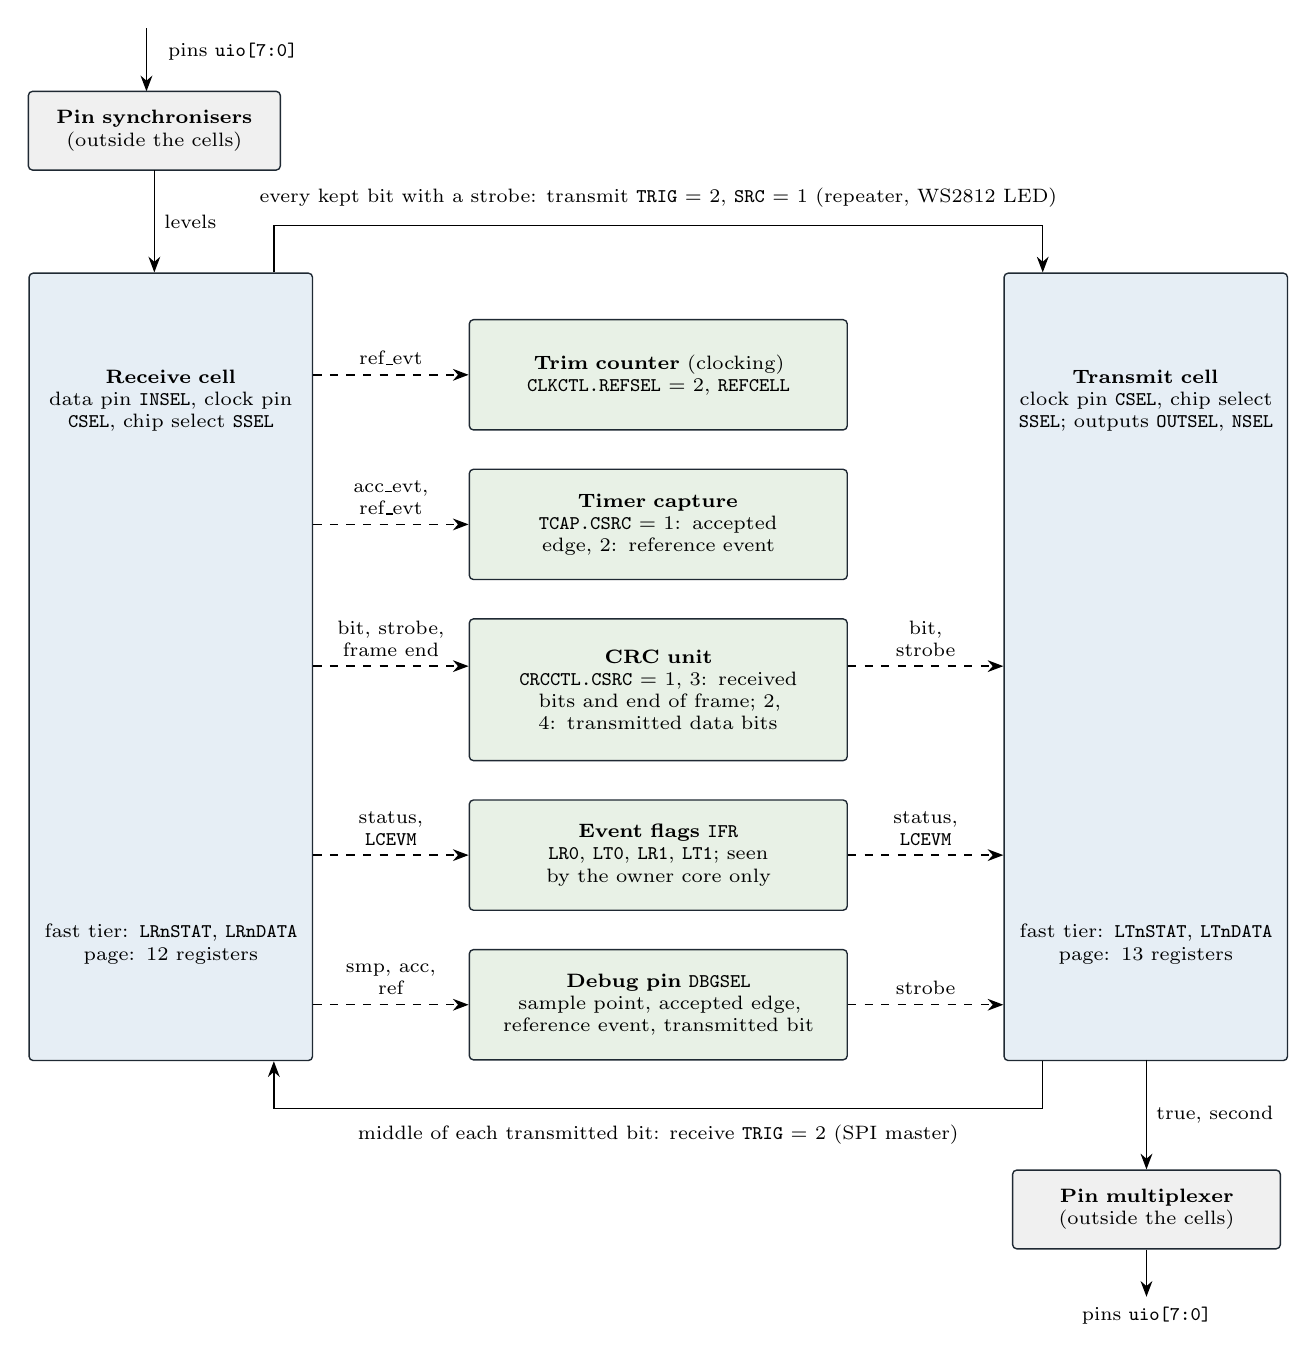
\begin{tikzpicture}[x=1mm,y=1mm,
  b/.style={blk,font=\scriptsize,inner sep=2pt,minimum height=14mm,minimum width=48mm,text width=45mm},
  ev/.style={ar,dashed}]
  % pins and synchronisers
  \draw[ar] (15,144) -- (15,136) ;
  \node[lbl,anchor=west] at (16.5,141) {pins \texttt{uio[7:0]}};
  \node[blk,fill=fillD,font=\scriptsize,inner sep=2pt,minimum width=32mm,text width=30mm,minimum height=10mm] (sy) at (16,131) {\textbf{Pin synchronisers}\\ (outside the cells)};
  \draw[ar] (16,126) -- (16,113) node[pos=0.5,right,lbl]{levels};
  % cells
  \node[blk,fill=fillA,anchor=north west,minimum width=36mm,minimum height=100mm,align=center,font=\scriptsize,text width=33mm,inner sep=2pt] (R) at (0,113) {\textbf{Receive cell}\\ data pin \reg{INSEL}, clock pin \reg{CSEL}, chip select \reg{SSEL}\\[62mm] fast tier: \reg{LRnSTAT}, \reg{LRnDATA}\\ page: 12 registers};
  \node[blk,fill=fillA,anchor=north east,minimum width=36mm,minimum height=100mm,align=center,font=\scriptsize,text width=33mm,inner sep=2pt] (T) at (160,113) {\textbf{Transmit cell}\\ clock pin \reg{CSEL}, chip select \reg{SSEL}; outputs \reg{OUTSEL}, \reg{NSEL}\\[62mm] fast tier: \reg{LTnSTAT}, \reg{LTnDATA}\\ page: 13 registers};
  % consumers
  \node[b,fill=fillC] (tc) at (80,100) {\textbf{Trim counter} (clocking)\\ \reg{CLKCTL.REFSEL} = 2, \reg{REFCELL}};
  \node[b,fill=fillC] (cap) at (80,81) {\textbf{Timer capture}\\ \reg{TCAP.CSRC} = 1: accepted edge, 2: reference event};
  \node[b,fill=fillC,minimum height=18mm] (crc) at (80,60) {\textbf{CRC unit}\\ \reg{CRCCTL.CSRC} = 1, 3: received bits and end of frame; 2, 4: transmitted data bits};
  \node[b,fill=fillC] (evf) at (80,39) {\textbf{Event flags} \reg{IFR}\\ \reg{LR0}, \reg{LT0}, \reg{LR1}, \reg{LT1}; seen by the owner core only};
  \node[b,fill=fillC] (dbg) at (80,20) {\textbf{Debug pin} \reg{DBGSEL}\\ sample point, accepted edge, reference event, transmitted bit};
  % arrows from the receive cell
  \draw[ev] (R.east |- tc.west) -- (tc.west) node[midway,above,lbl]{ref\_evt};
  \draw[ev] (R.east |- cap.west) -- (cap.west) node[midway,above,lbl,align=center]{acc\_evt,\\ ref\_evt};
  \draw[ev] ($(R.east |- crc.west)+(0,3)$) -- ($(crc.west)+(0,3)$) node[midway,above,lbl,align=center]{bit, strobe,\\ frame end};
  \draw[ev] (R.east |- evf.west) -- (evf.west) node[midway,above,lbl,align=center]{status,\\ \reg{LCEVM}};
  \draw[ev] (R.east |- dbg.west) -- (dbg.west) node[midway,above,lbl,align=center]{smp, acc,\\ ref};
  % arrows from the transmit cell
  \draw[ev] ($(crc.east)+(0,3)$) -- ($(T.west |- crc.east)+(0,3)$) node[midway,above,lbl,align=center]{bit,\\ strobe};
  \draw[ev] (evf.east) -- (T.west |- evf.east) node[midway,above,lbl,align=center]{status,\\ \reg{LCEVM}};
  \draw[ev] (dbg.east) -- (T.west |- dbg.east) node[midway,above,lbl,align=center]{strobe};
  % links between the cells
  \draw[ar] ($(R.north east)+(-5,0)$) -- ++(0,6) -| ($(T.north west)+(5,0)$);
  \node[lbl,anchor=south] at (80,120) {every kept bit with a strobe: transmit \reg{TRIG} = 2, \reg{SRC} = 1 (repeater, WS2812 LED)};
  \draw[ar] ($(T.south west)+(5,0)$) -- ++(0,-6) -| ($(R.south east)+(-5,0)$);
  \node[lbl,anchor=north] at (80,6) {middle of each transmitted bit: receive \reg{TRIG} = 2 (SPI master)};
  % pin multiplexer
  \node[blk,fill=fillD,font=\scriptsize,inner sep=2pt,minimum width=34mm,text width=32mm,minimum height=10mm] (pm) at (142,-6) {\textbf{Pin multiplexer}\\ (outside the cells)};
  \draw[ar] (142,13) -- (pm.north) node[midway,right,lbl]{true, second};
  \draw[ar] (pm.south) -- ++(0,-6) node[below,lbl]{pins \texttt{uio[7:0]}};
\end{tikzpicture}
}
\caption{A pair of line cells and its connections.}
\end{figure}

\paragraph{Time unit and timer values.} All times in a cell are counted in its time unit: $2^{\mathtt{PRE}}$
clock cycles of the peripheral clock, or half a clock cycle for a receive cell with \reg{UNIT} = 1. Each cell has
an 8-bit timer. Its reload values A, B and C are registers; the value 0 means 256.

\begin{itemize}
\item Receive cell: A is the time from an accepted edge to the first sample. B is the time from one sample to
the next, and the timeout that sets \reg{IDLE} while the cell waits for an edge.
\item Transmit cell: B is the bit time, or one of two periods per bit with \reg{TWOPH}. In compare mode A is the
high time for a one and C the high time for a zero.
\end{itemize}

\paragraph{Receive cell.}

\begin{figure}[H]
\centering
\resizebox{\textwidth}{!}{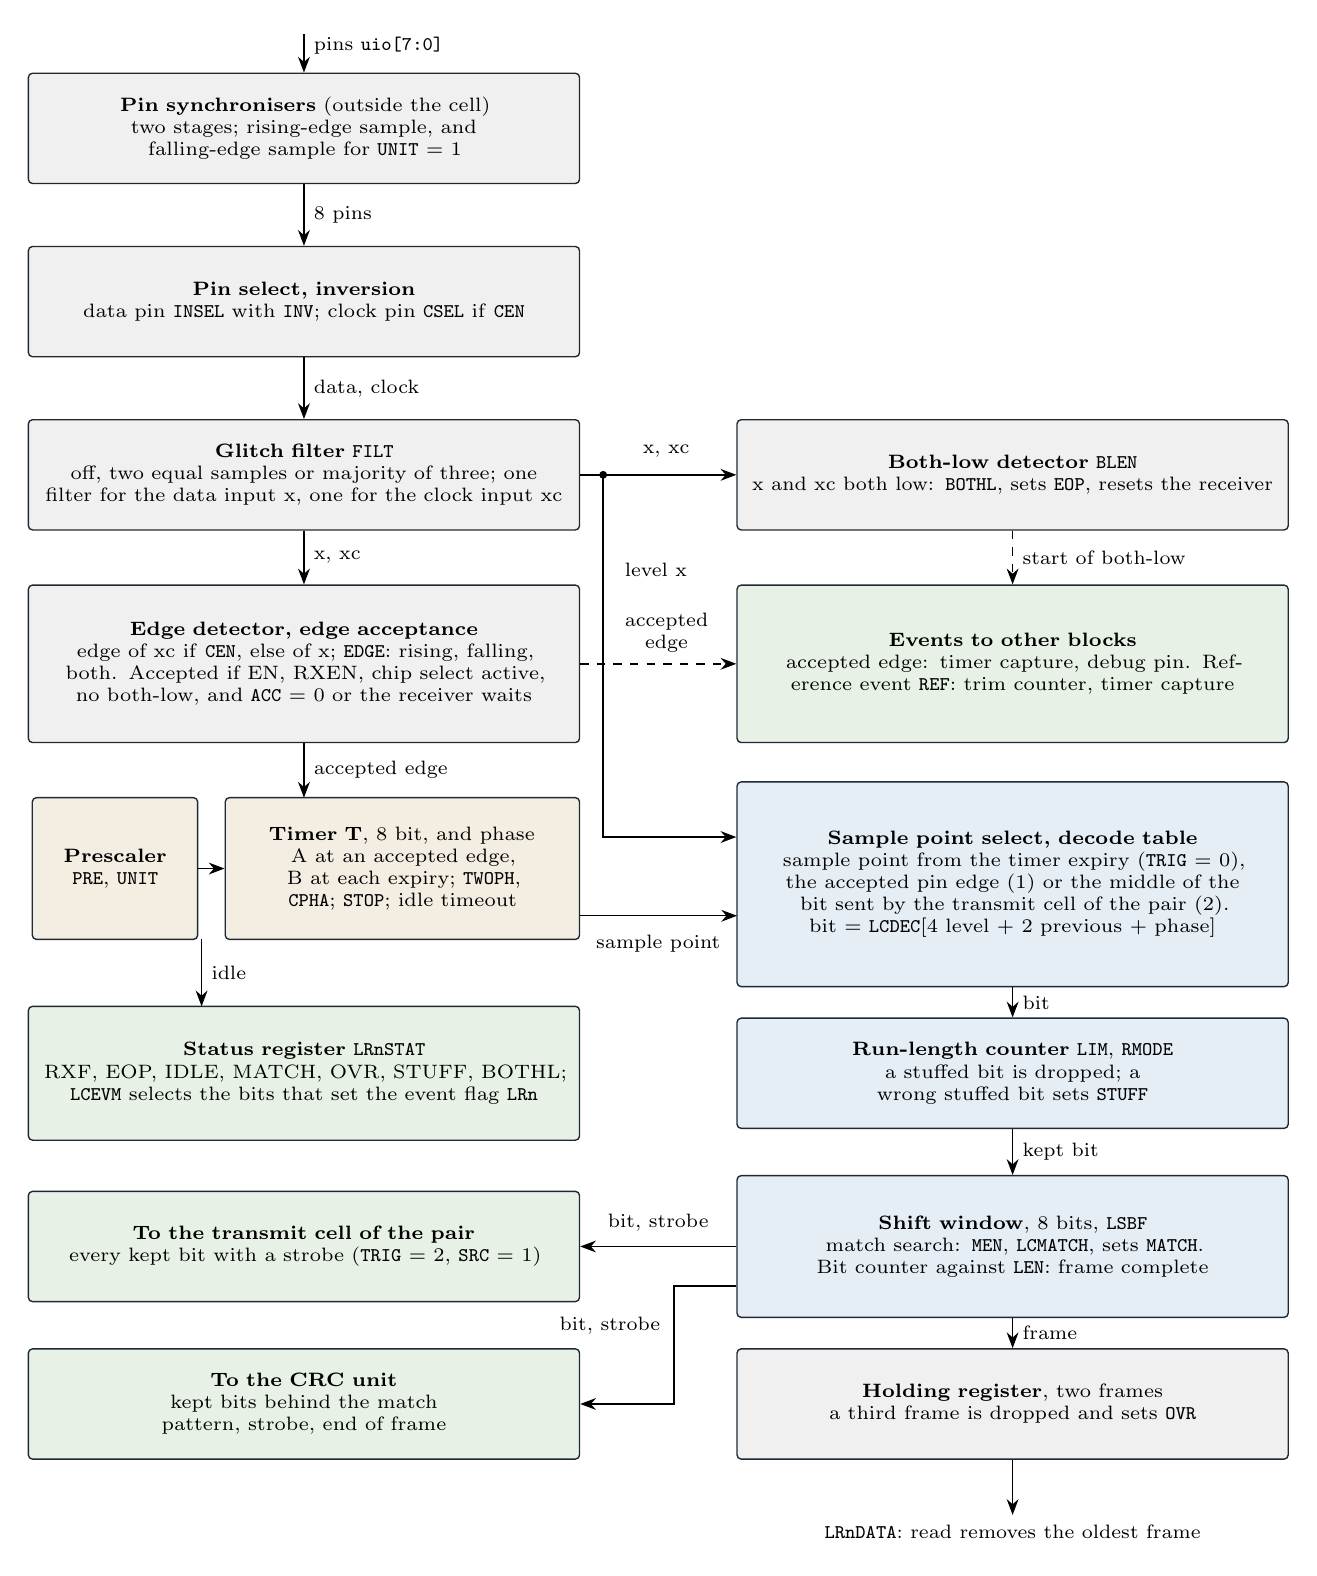
\begin{tikzpicture}[x=1mm,y=1mm,
  b/.style={blk,font=\scriptsize,inner sep=2pt,minimum height=14mm,minimum width=70mm,text width=66mm},
  ev/.style={ar,dashed}]
  % left lane: input path and timing
  \node[b,fill=fillD] (sy) at (35,140) {\textbf{Pin synchronisers} (outside the cell)\\ two stages; rising-edge sample, and falling-edge sample for \reg{UNIT} = 1};
  \node[b,fill=fillD] (ps) at (35,118) {\textbf{Pin select, inversion}\\ data pin \reg{INSEL} with \reg{INV}; clock pin \reg{CSEL} if \reg{CEN}};
  \node[b,fill=fillD] (fl) at (35,96) {\textbf{Glitch filter} \reg{FILT}\\ off, two equal samples or majority of three; one filter for the data input x, one for the clock input xc};
  \node[b,fill=fillD,minimum height=20mm] (ed) at (35,72) {\textbf{Edge detector, edge acceptance}\\ edge of xc if \reg{CEN}, else of x; \reg{EDGE}: rising, falling, both. Accepted if EN, RXEN, chip select active, no both-low, and \reg{ACC} = 0 or the receiver waits};
  \node[b,fill=fillB,minimum width=21mm,text width=18mm,minimum height=18mm] (pre) at (11,46) {\textbf{Prescaler}\\ \reg{PRE}, \reg{UNIT}};
  \node[b,fill=fillB,minimum width=45mm,text width=42mm,minimum height=18mm] (tm) at (47.5,46) {\textbf{Timer T}, 8 bit, and phase\\ A at an accepted edge, B at each expiry; \reg{TWOPH}, \reg{CPHA}; \reg{STOP}; idle timeout};
  \node[b,fill=fillC,minimum height=17mm] (st) at (35,20) {\textbf{Status register} \reg{LRnSTAT}\\ RXF, EOP, IDLE, MATCH, OVR, STUFF, BOTHL; \reg{LCEVM} selects the bits that set the event flag \reg{LRn}};
  \node[b,fill=fillC] (pl) at (35,-2) {\textbf{To the transmit cell of the pair}\\ every kept bit with a strobe (\reg{TRIG} = 2, \reg{SRC} = 1)};
  \node[b,fill=fillC] (cr) at (35,-22) {\textbf{To the CRC unit}\\ kept bits behind the match pattern, strobe, end of frame};
  % right lane: decoding
  \node[b,fill=fillD] (bl) at (125,96) {\textbf{Both-low detector} \reg{BLEN}\\ x and xc both low: \reg{BOTHL}, sets \reg{EOP}, resets the receiver};
  \node[b,fill=fillC,minimum height=20mm] (o1) at (125,72) {\textbf{Events to other blocks}\\ accepted edge: timer capture, debug pin. Reference event \reg{REF}: trim counter, timer capture};
  \node[b,fill=fillA,minimum height=26mm] (dc) at (125,44) {\textbf{Sample point select, decode table}\\ sample point from the timer expiry (\reg{TRIG} = 0), the accepted pin edge (1) or the middle of the bit sent by the transmit cell of the pair (2).\\ bit = \reg{LCDEC}[4 level + 2 previous + phase]};
  \node[b,fill=fillA] (rl) at (125,20) {\textbf{Run-length counter} \reg{LIM}, \reg{RMODE}\\ a stuffed bit is dropped; a wrong stuffed bit sets \reg{STUFF}};
  \node[b,fill=fillA,minimum height=18mm] (sh) at (125,-2) {\textbf{Shift window}, 8 bits, \reg{LSBF}\\ match search: \reg{MEN}, \reg{LCMATCH}, sets \reg{MATCH}. Bit counter against \reg{LEN}: frame complete};
  \node[b,fill=fillD] (hr) at (125,-22) {\textbf{Holding register}, two frames\\ a third frame is dropped and sets \reg{OVR}};
  % arrows, left lane
  \draw[ar] (35,152) -- (sy.north) node[pos=0.3,right,lbl]{pins \texttt{uio[7:0]}};
  \draw[ar] (sy) -- (ps) node[midway,right,lbl]{8 pins};
  \draw[ar] (ps) -- (fl) node[midway,right,lbl]{data, clock};
  \draw[ar] (fl) -- (ed) node[midway,right,lbl]{x, xc};
  \draw[ar] (35,62) -- (35,55) node[pos=0.5,right,lbl]{accepted edge};
  \draw[ar] (pre) -- (tm) node[midway,above,lbl]{};
  \draw[ar] (22,37) -- (22,28.5) node[midway,right,lbl]{idle};
  % cross links
  \draw[ar] (fl.east) -- (bl.west);
  \node[lbl] at (81,99) {x, xc};
  \draw[ar] (73,96) -- (73,50) -- ($(dc.west)+(0,6)$);
  \fill (73,96) circle (0.5);
  \node[lbl,anchor=west] at (74.5,84) {level x};
  \draw[ev] (ed.east) -- (o1.west);
  \node[lbl,anchor=west] at (74.5,76) {accepted\\ edge};
  \draw[ev] (bl.south) -- (o1.north) node[midway,right,lbl]{start of both-low};
  \draw[ar] (70,40) -- (90,40);
  \node[lbl] at (80,36.5) {sample point};
  % arrows, right lane
  \draw[ar] (dc) -- (rl) node[midway,right,lbl]{bit};
  \draw[ar] (rl) -- (sh) node[midway,right,lbl]{kept bit};
  \draw[ar] (sh.south) -- (hr.north) node[midway,right,lbl]{frame};
  \draw[ar] (sh.west) -- (pl.east);
  \node[lbl] at (80,1) {bit, strobe};
  \draw[ar] ($(sh.west)+(0,-5)$) -| (82,-22) -- (cr.east);
  \node[lbl,anchor=east] at (81.5,-12) {bit, strobe};
  \draw[ar] (hr.south) -- ++(0,-7) node[below,lbl]{\reg{LRnDATA}: read removes the oldest frame};
\end{tikzpicture}
}
\caption{Receive cell. Left: input path and timing. Right: decoding and data path.}
\end{figure}

\begin{enumerate}
\item \textbf{Input.} One of the eight bidirectional pins (\reg{INSEL}), optionally inverted (\reg{INV}) and filtered
(\reg{FILT}: two equal samples or majority of three). The level reaches the cell two clock cycles after it is at
the pin.
\item \textbf{Edge detector.} It watches the input pin, or a separate clock pin (\reg{CSEL}, \reg{CEN}). \reg{EDGE}
selects rising, falling or both. An edge is accepted always, or only while the cell waits (\reg{ACC}).
\item \textbf{Sample point.} \reg{TRIG} selects where it comes from:
  \begin{itemize}
  \item the timer: an accepted edge loads A, each expiry is a sample point and loads B. \reg{STOP} selects whether
  the timer keeps running, or the cell waits for the next edge after each sample or after each frame;
  \item an accepted edge of the clock pin: one sample per clock edge (clocked reception);
  \item the middle of each bit that the transmit cell of the pair sends.
  \end{itemize}
\item \textbf{Decoding.} At a sample point the 8-entry decode table gives the bit from the pin level, the
previous sample and the phase. One table value selects level, inverted level or NRZI.
\item \textbf{Bit stuffing.} With \reg{LIM} not 0 a run-length counter drops the bit that follows \reg{LIM} ones (or
equal bits, \reg{RMODE}). If that bit does not have the expected value, \reg{STUFF} is set.
\item \textbf{Match pattern.} With \reg{MEN} the cell delivers no frame after it was enabled or reset until the last
eight bits equal \reg{LCMATCH}. Then \reg{MATCH} is set and the next bit starts the first frame. This aligns the
frames on a sync pattern or a start-of-frame delimiter.
\item \textbf{Frames.} After \reg{LEN}+1 bits the frame moves to the holding register, which holds two frames, and
\reg{RXF} is set. Reading \reg{LRnDATA} returns the oldest frame. A frame that completes while two are waiting is
lost and sets \reg{OVR}.
\item \textbf{Idle and receiver reset.} While the cell waits for an edge, B runs as a timeout; when it expires, the
line is idle. If the timer keeps running (\reg{STOP} = 0), the line is idle at the eighth expiry in a row without an
accepted edge. \reg{IDLE} is then set and the receiver is reset: an incomplete frame is discarded and the search
for the match pattern starts again, so the next packet is aligned anew. Frames in the holding register are
kept. The receiver is also reset by the start of both pins low, by an inactive chip select and by clearing
\reg{RXEN}.
\item \textbf{Both pins low.} With \reg{BLEN} the cell reports when the input pin and the pin \reg{CSEL} are both
low (\reg{BOTHL} as a level, \reg{EOP} stored). This is the end of packet of USB.
\item \textbf{Events to other blocks.} Each kept bit goes to the transmit cell of the pair and, after the match
pattern, to the CRC unit. A selected event (\reg{REF}) goes to the trim counter and the timer capture.
\end{enumerate}

\paragraph{Transmit cell.}

\begin{figure}[H]
\centering
\resizebox{\textwidth}{!}{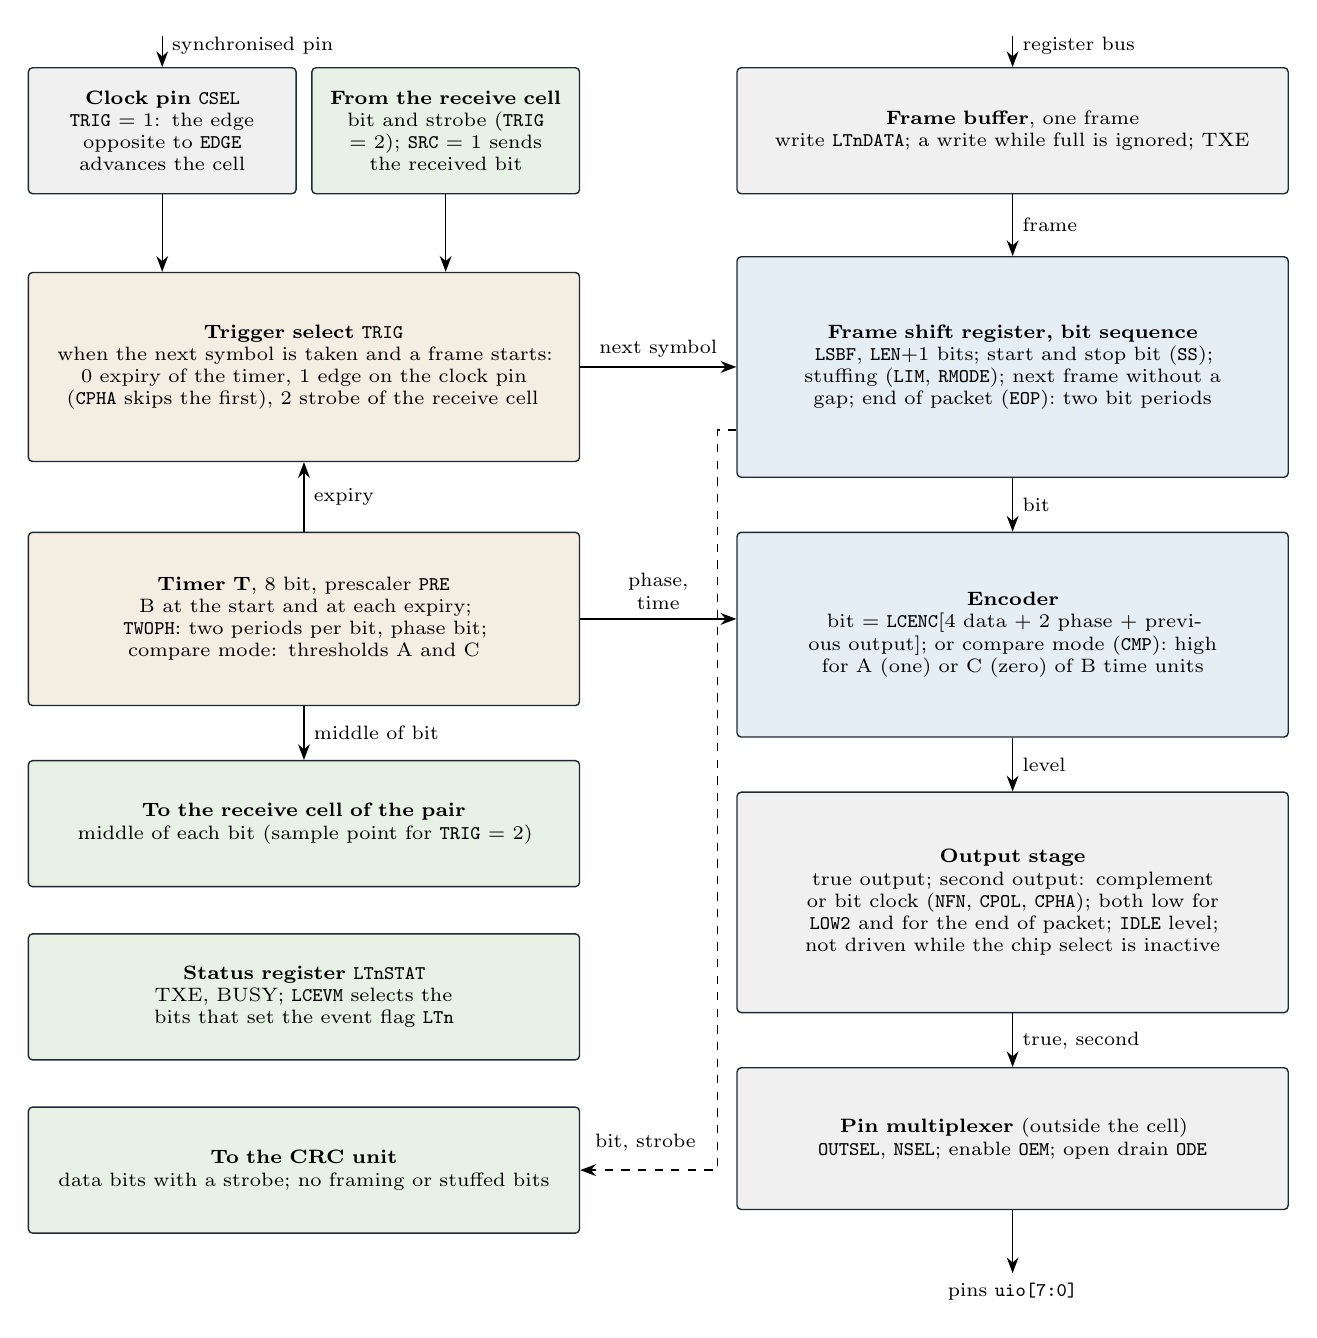
\begin{tikzpicture}[x=1mm,y=1mm,
  b/.style={blk,font=\scriptsize,inner sep=2pt,minimum height=14mm,minimum width=70mm,text width=66mm},
  ev/.style={ar,dashed}]
  % left lane: trigger and timing
  \node[b,fill=fillD,minimum width=34mm,text width=31mm,minimum height=16mm] (cp) at (17,150) {\textbf{Clock pin} \reg{CSEL}\\ \reg{TRIG} = 1: the edge opposite to \reg{EDGE} advances the cell};
  \node[b,fill=fillC,minimum width=34mm,text width=31mm,minimum height=16mm] (rc) at (53,150) {\textbf{From the receive cell}\\ bit and strobe (\reg{TRIG} = 2); \reg{SRC} = 1 sends the received bit};
  \node[b,fill=fillB,minimum height=24mm] (tr) at (35,120) {\textbf{Trigger select} \reg{TRIG}\\ when the next symbol is taken and a frame starts: 0 expiry of the timer, 1 edge on the clock pin (\reg{CPHA} skips the first), 2 strobe of the receive cell};
  \node[b,fill=fillB,minimum height=22mm] (tm) at (35,88) {\textbf{Timer T}, 8 bit, prescaler \reg{PRE}\\ B at the start and at each expiry; \reg{TWOPH}: two periods per bit, phase bit; compare mode: thresholds A and C};
  \node[b,fill=fillC,minimum height=16mm] (tmid) at (35,62) {\textbf{To the receive cell of the pair}\\ middle of each bit (sample point for \reg{TRIG} = 2)};
  \node[b,fill=fillC,minimum height=16mm] (stat) at (35,40) {\textbf{Status register} \reg{LTnSTAT}\\ TXE, BUSY; \reg{LCEVM} selects the bits that set the event flag \reg{LTn}};
  \node[b,fill=fillC,minimum height=16mm] (crc) at (35,18) {\textbf{To the CRC unit}\\ data bits with a strobe; no framing or stuffed bits};
  % right lane: data path
  \node[b,fill=fillD,minimum height=16mm] (fb) at (125,150) {\textbf{Frame buffer}, one frame\\ write \reg{LTnDATA}; a write while full is ignored; TXE};
  \node[b,fill=fillA,minimum height=28mm] (sq) at (125,120) {\textbf{Frame shift register, bit sequence}\\ \reg{LSBF}, \reg{LEN}+1 bits; start and stop bit (\reg{SS}); stuffing (\reg{LIM}, \reg{RMODE}); next frame without a gap; end of packet (\reg{EOP}): two bit periods};
  \node[b,fill=fillA,minimum height=26mm] (en) at (125,86) {\textbf{Encoder}\\ bit = \reg{LCENC}[4 data + 2 phase + previous output]; or compare mode (\reg{CMP}): high for A (one) or C (zero) of B time units};
  \node[b,fill=fillD,minimum height=28mm] (os) at (125,52) {\textbf{Output stage}\\ true output; second output: complement or bit clock (\reg{NFN}, \reg{CPOL}, \reg{CPHA}); both low for \reg{LOW2} and for the end of packet; \reg{IDLE} level; not driven while the chip select is inactive};
  \node[b,fill=fillD,minimum height=18mm] (pm) at (125,22) {\textbf{Pin multiplexer} (outside the cell)\\ \reg{OUTSEL}, \reg{NSEL}; enable \reg{OEM}; open drain \reg{ODE}};
  % arrows
  \draw[ar] (17,162) -- (cp.north) node[pos=0.3,right,lbl]{synchronised pin};
  \draw[ar] (cp.south) -- (cp.south |- tr.north);
  \draw[ar] (rc.south) -- (rc.south |- tr.north);
  \draw[ar] (tm.north) -- (tm.north |- tr.south) node[pos=0.5,right,lbl]{expiry};
  \draw[ar] (tr.east) -- (sq.west |- tr.east) node[pos=0.5,above,lbl]{next symbol};
  \draw[ar] (tm.east) -- (en.west |- tm.east) node[pos=0.5,above,lbl,align=center]{phase,\\ time};
  \draw[ar] (tm.south) -- (tmid.north) node[midway,right,lbl]{middle of bit};
  \draw[ar] (fb) -- (sq) node[midway,right,lbl]{frame};
  \draw[ar] (sq) -- (en) node[midway,right,lbl]{bit};
  \draw[ar] (en) -- (os) node[midway,right,lbl]{level};
  \draw[ar] (os) -- (pm) node[midway,right,lbl]{true, second};
  \draw[ar] (pm.south) -- ++(0,-8) node[below,lbl]{pins \texttt{uio[7:0]}};
  \draw[ar] (125,162) -- (fb.north) node[pos=0.3,right,lbl]{register bus};
  \draw[ev] ($(sq.west)+(0,-8)$) -| (87.5,18) -- (crc.east);
  \node[lbl,anchor=east] at (86,21.5) {bit, strobe};
\end{tikzpicture}
}
\caption{Transmit cell.}
\end{figure}

\begin{enumerate}
\item \textbf{Frame buffer.} Writing \reg{LTnDATA} stores one frame and clears \reg{TXE}. When the shift register
is free the frame moves there, \reg{TXE} is set again and \reg{BUSY} is set. A frame written before the last bit
of the current frame ends follows without a gap.
\item \textbf{Bit sequence.} \reg{LEN}+1 bits in the selected order; with \reg{SS} a start bit before and a stop bit
after them; with \reg{LIM} not 0 a stuffed bit after \reg{LIM} ones.
\item \textbf{Advance.} \reg{TRIG} selects what moves the cell to the next bit: the timer (B per bit, or two
periods of B with \reg{TWOPH}), an edge on a clock pin (clocked transmission as a slave), or each bit that the
receive cell of the pair delivers. With \reg{SRC} the bit value also comes from the receive cell; the pair then
forwards a bit stream with new timing and a new line code.
\item \textbf{Line code.} The 8-entry encode table gives the output level from the data bit, the phase and the
previous output: NRZ, NRZI, Manchester. In compare mode (\reg{CMP}) the output is high for A or C time units at
the start of each bit of B time units.
\item \textbf{Outputs.} The true output goes to pin \reg{OUTSEL}. The second output (pin \reg{NSEL}) is the complement
of the true output or, with \reg{NFN}, a bit clock with polarity \reg{CPOL} and phase \reg{CPHA}. \reg{OEM} selects
whether the pins are driven as the direction register says, always, or only while the cell is busy.
\item \textbf{End of a transmission.} When the last bit ends and the buffer is empty, the outputs take the idle
level (\reg{IDLE}) and \reg{BUSY} is cleared. With \reg{EOP} both outputs are low for two bit times first.
\end{enumerate}

\paragraph{Additional frame bit.} With \reg{PAR} in \reg{LCX} not 0 every frame has one more bit after its data
bits; in the transmit cell it comes before the stop bit. The transmit cell computes an odd or even parity bit,
or sends the bit \reg{X9} that was in \reg{LCX} when the frame was written (ninth data bit). The receive cell
completes the frame with the additional bit, stores it with the frame and shows the bit of the oldest frame in
\reg{X9}; \reg{X9} is read before \reg{LRnDATA}. A wrong parity sets \reg{FERR} in the status register. The
additional bit is timed, encoded and counted for stuffing like a data bit. It is not shifted into the match
window and gives no strobe to the other cell of the pair or to the CRC unit. A transmit cell with a ninth data
bit that is always 1 sends two stop bits.

\paragraph{Start at the shift edge.} A transmit cell that is clocked by a pin puts out the first bit of a frame
when the frame is written. With \reg{ESTR} = 1 it waits and puts out the first bit at the first shift edge after
the write, so its output changes only at shift edges. This is the setting for the data line of an I2C slave,
where a change while the clock is high is a start or stop condition. \reg{CPHA} has no effect with \reg{ESTR} = 1.

\paragraph{Bus conditions.} With \reg{BCD} = 1 a receive cell with a clock pin watches its two inputs in every
clock cycle. A falling edge of the data input while the clock input is high sets the flag \reg{STA}, a rising
edge sets \reg{STP}. Both reset the bit count of the receiver, so the next frame starts with the next clock
edge; frames in the holding register are kept. A data edge in the same clock cycle as a clock edge is not a
condition. With \reg{EC} in \reg{LCEC} not 0 the cell counts falling edges of the data input while the clock
input is low; a clock edge clears the count and the flag \reg{ECF} is set when the count reaches \reg{EC}. The
three flags are in \reg{LCX}. They are cleared by writing a one, which also writes the configuration bits of
\reg{LCX}, and they set the event flag of the cell with \reg{BEV} = 1.

\paragraph{Chip select, pins and events.} A cell with \reg{SSEN} is held in reset and does not drive its pins
while its chip select pin is inactive. A pin whose output is claimed by a transmit cell does not follow the
port register. Each pair belongs to one core (\reg{LCOWN}); only that core can access its registers and sees its
event flags. A status bit selected in \reg{LCEVM} sets the event flag of the cell, on which the core can wait.

\paragraph{Fixed delays.} A pin level reaches the receive cell two clock cycles after it is at the pin. A frame
written to \reg{LTnDATA} appears at the pin three clock cycles after the write when the transmitter is idle.

\subsection{Configuration examples}

\begin{table}[H]
\centering\small
\begin{tabularx}{\linewidth}{@{}lLL@{}}
\toprule
Protocol & Role and rate in simulation & Remarks \\
\midrule
UART & 8 data bits, optional parity (odd, even) or ninth bit, 1 stop bit, or 2 stop bits on transmit without parity; 2 clock cycles per bit and slower; bit time tolerance of the receiver $\pm 5.3\,\%$ at 16 cycles per bit and above & stop bit and start bit are not checked by one cell\\
SPI & master in modes 0 to 3 at 8 cycles per bit and slower (7.5\,MHz); slave with data out down to 12 cycles per bit (5\,MHz) & no underrun indication as slave \\
I2C & slave with line cells at 100 and 400\,kHz, start and stop from the bus condition flags; master in firmware with clock stretching, arbitration and bus recovery & acknowledge by firmware; no clock stretching by hardware as slave \\
WS2812 & controller at 800\,kbit/s; LED with forwarding & forwarding keeps the bit period of the input \\
USB low-speed & device (HID with enumeration) from the 60\,MHz clock or from the internal oscillator trimmed by the bus & core clock of 15\,MHz or more for the device stack \\
10BASE-T & frames up to 1\,518 bytes, frame check with the CRC unit, ARP and ping endpoint & idle pulse single-ended by firmware; no link pulses; line driver and transformer external \\
\bottomrule
\end{tabularx}
\caption{Protocols with tested configurations. Rates are from RTL simulation with ideal signals; rates on
real pins: \tbd.}
\end{table}

The following examples give the register settings and a timing diagram for the main ways of using a cell. The
diagrams are drawn from RTL simulation of the complete chip, one column per clock cycle, and the settings are
read from the same simulation. The rates are low so that single clock cycles are visible; for other rates only
A, B, C and \reg{PRE} change. An arrow on a row marks the clock cycle of an event. The rows ``pin sampled'' and
``edge accepted'' show the time at the pin; the status bits follow two cycles later. Registers that are not
listed are zero.

\paragraph{Example 1: start-stop framing (UART).} 8 clock cycles per bit, one frame \texttt{0x53}; the receive cell
listens on the pin of the transmit cell. For another rate: B = bit time, A = 1.5 bit times, with \reg{PRE} so that
both fit into 8 bit (115\,200 baud at 60\,MHz: \reg{PRE} = 2, B = 130, A = 195).

{\small\begin{tabularx}{\linewidth}{@{}l l L l L@{}}
\toprule
 & \multicolumn{2}{l}{Transmit cell} & \multicolumn{2}{l}{Receive cell} \\
\midrule
\texttt{LCCTRL} & \texttt{0xA0} & enabled; transmitter on & \texttt{0xC0} & enabled; receiver on \\
\texttt{LCPIN} & \texttt{0x01} & pins always driven & \texttt{0x00} & input pin 0 \\
\texttt{LCOUT} & \texttt{0x10} & true output on pin 0 &  &  \\
\texttt{LCTIM} & \texttt{0x00} & next bit from the timer & \texttt{0xB0} & falling edge; accepted only while waiting; wait after each frame \\
\texttt{LCA} &  &  & \texttt{12} & 12 time units from the edge to the first sample \\
\texttt{LCB} & \texttt{8} & 8 time units per bit & \texttt{8} & 8 time units between samples, and idle timeout \\
\texttt{LCDEC} &  &  & \texttt{0xF0} & level \\
\texttt{LCENC} & \texttt{0xF0} & NRZ &  &  \\
\texttt{LCSH} & \texttt{0xF1} & 8 bits; LSB first; start and stop bit & \texttt{0xF0} & 8 bits; LSB first \\
\texttt{LCRUN} & \texttt{0x04} & idle level high &  &  \\
\texttt{LCEVM} &  &  & \texttt{0x80} & event flag on \texttt{RXF} \\
\bottomrule
\end{tabularx}
}

\begin{figure}[H]
\centering
% SPDX-FileCopyrightText: (c) 2026 Tim S. B. (GitHub: cpldcpu)
% SPDX-License-Identifier: Apache-2.0
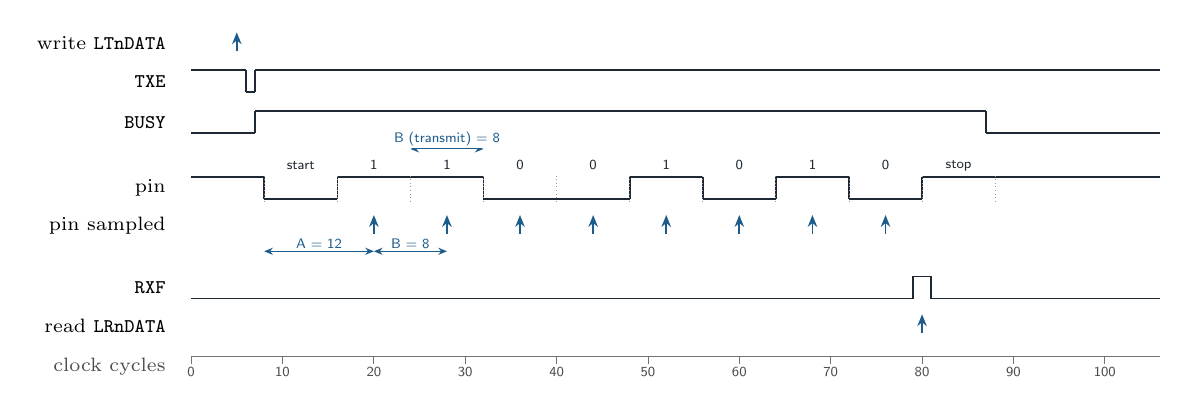
\begin{tikzpicture}[x=1mm,y=1mm]
\node[lbl,anchor=east] at (25.00,-3.40) {write \texttt{LTnDATA}};
\draw[accent,line width=0.6pt,-{Stealth[length=1.5mm,width=1.2mm]}] (32.80,-4.40) -- ++(0,2.4);
\node[lbl,anchor=east] at (25.00,-8.20) {\texttt{TXE}};
\draw[ink,line width=0.6pt] (27.00,-6.80) -- (33.96,-6.80);
\draw[ink,line width=0.6pt] (33.96,-6.80) -- (33.96,-9.60);
\draw[ink,line width=0.6pt] (33.96,-9.60) -- (35.12,-9.60);
\draw[ink,line width=0.6pt] (35.12,-9.60) -- (35.12,-6.80);
\draw[ink,line width=0.6pt] (35.12,-6.80) -- (150.00,-6.80);
\node[lbl,anchor=east] at (25.00,-13.40) {\texttt{BUSY}};
\draw[ink,line width=0.6pt] (27.00,-14.80) -- (35.12,-14.80);
\draw[ink,line width=0.6pt] (35.12,-14.80) -- (35.12,-12.00);
\draw[ink,line width=0.6pt] (35.12,-12.00) -- (127.95,-12.00);
\draw[ink,line width=0.6pt] (127.95,-12.00) -- (127.95,-14.80);
\draw[ink,line width=0.6pt] (127.95,-14.80) -- (150.00,-14.80);
\node[lbl,anchor=east] at (25.00,-21.80) {pin};
\draw[ink,line width=0.6pt] (27.00,-20.40) -- (36.28,-20.40);
\draw[ink,line width=0.6pt] (36.28,-20.40) -- (36.28,-23.20);
\draw[ink,line width=0.6pt] (36.28,-23.20) -- (45.57,-23.20);
\draw[ink,line width=0.6pt] (45.57,-23.20) -- (45.57,-20.40);
\draw[ink,line width=0.6pt] (45.57,-20.40) -- (64.13,-20.40);
\draw[ink,line width=0.6pt] (64.13,-20.40) -- (64.13,-23.20);
\draw[ink,line width=0.6pt] (64.13,-23.20) -- (82.70,-23.20);
\draw[ink,line width=0.6pt] (82.70,-23.20) -- (82.70,-20.40);
\draw[ink,line width=0.6pt] (82.70,-20.40) -- (91.98,-20.40);
\draw[ink,line width=0.6pt] (91.98,-20.40) -- (91.98,-23.20);
\draw[ink,line width=0.6pt] (91.98,-23.20) -- (101.26,-23.20);
\draw[ink,line width=0.6pt] (101.26,-23.20) -- (101.26,-20.40);
\draw[ink,line width=0.6pt] (101.26,-20.40) -- (110.55,-20.40);
\draw[ink,line width=0.6pt] (110.55,-20.40) -- (110.55,-23.20);
\draw[ink,line width=0.6pt] (110.55,-23.20) -- (119.83,-23.20);
\draw[ink,line width=0.6pt] (119.83,-23.20) -- (119.83,-20.40);
\draw[ink,line width=0.6pt] (119.83,-20.40) -- (150.00,-20.40);
\node[font=\tiny\sffamily,text=ink,inner sep=0.6pt,anchor=center] at (40.92,-18.90) {start};
\node[font=\tiny\sffamily,text=ink,inner sep=0.6pt,anchor=center] at (50.21,-18.90) {1};
\node[font=\tiny\sffamily,text=ink,inner sep=0.6pt,anchor=center] at (59.49,-18.90) {1};
\node[font=\tiny\sffamily,text=ink,inner sep=0.6pt,anchor=center] at (68.77,-18.90) {0};
\node[font=\tiny\sffamily,text=ink,inner sep=0.6pt,anchor=center] at (78.06,-18.90) {0};
\node[font=\tiny\sffamily,text=ink,inner sep=0.6pt,anchor=center] at (87.34,-18.90) {1};
\node[font=\tiny\sffamily,text=ink,inner sep=0.6pt,anchor=center] at (96.62,-18.90) {0};
\node[font=\tiny\sffamily,text=ink,inner sep=0.6pt,anchor=center] at (105.91,-18.90) {1};
\node[font=\tiny\sffamily,text=ink,inner sep=0.6pt,anchor=center] at (115.19,-18.90) {0};
\node[font=\tiny\sffamily,text=ink,inner sep=0.6pt,anchor=center] at (124.47,-18.90) {stop};
\draw[black!40,line width=0.3pt,densely dotted] (36.28,-23.50) -- (36.28,-19.90);
\draw[black!40,line width=0.3pt,densely dotted] (45.57,-23.50) -- (45.57,-19.90);
\draw[black!40,line width=0.3pt,densely dotted] (54.85,-23.50) -- (54.85,-19.90);
\draw[black!40,line width=0.3pt,densely dotted] (64.13,-23.50) -- (64.13,-19.90);
\draw[black!40,line width=0.3pt,densely dotted] (73.42,-23.50) -- (73.42,-19.90);
\draw[black!40,line width=0.3pt,densely dotted] (82.70,-23.50) -- (82.70,-19.90);
\draw[black!40,line width=0.3pt,densely dotted] (91.98,-23.50) -- (91.98,-19.90);
\draw[black!40,line width=0.3pt,densely dotted] (101.26,-23.50) -- (101.26,-19.90);
\draw[black!40,line width=0.3pt,densely dotted] (110.55,-23.50) -- (110.55,-19.90);
\draw[black!40,line width=0.3pt,densely dotted] (119.83,-23.50) -- (119.83,-19.90);
\draw[black!40,line width=0.3pt,densely dotted] (129.11,-23.50) -- (129.11,-19.90);
\draw[accent,line width=0.4pt,{Stealth[length=1.1mm,width=0.9mm]}-{Stealth[length=1.1mm,width=0.9mm]}] (54.85,-16.80) -- (64.13,-16.80) node[midway,above,inner sep=0.8pt,font=\tiny\sffamily,text=accent,fill=white]{B (transmit) = 8};
\node[lbl,anchor=east] at (25.00,-26.60) {pin sampled};
\draw[accent,line width=0.6pt,-{Stealth[length=1.5mm,width=1.2mm]}] (50.21,-27.60) -- ++(0,2.4);
\draw[accent,line width=0.6pt,-{Stealth[length=1.5mm,width=1.2mm]}] (59.49,-27.60) -- ++(0,2.4);
\draw[accent,line width=0.6pt,-{Stealth[length=1.5mm,width=1.2mm]}] (68.77,-27.60) -- ++(0,2.4);
\draw[accent,line width=0.6pt,-{Stealth[length=1.5mm,width=1.2mm]}] (78.06,-27.60) -- ++(0,2.4);
\draw[accent,line width=0.6pt,-{Stealth[length=1.5mm,width=1.2mm]}] (87.34,-27.60) -- ++(0,2.4);
\draw[accent,line width=0.6pt,-{Stealth[length=1.5mm,width=1.2mm]}] (96.62,-27.60) -- ++(0,2.4);
\draw[accent,line width=0.6pt,-{Stealth[length=1.5mm,width=1.2mm]}] (105.91,-27.60) -- ++(0,2.4);
\draw[accent,line width=0.6pt,-{Stealth[length=1.5mm,width=1.2mm]}] (115.19,-27.60) -- ++(0,2.4);
\draw[accent,line width=0.4pt,{Stealth[length=1.1mm,width=0.9mm]}-{Stealth[length=1.1mm,width=0.9mm]}] (36.28,-29.80) -- (50.21,-29.80) node[midway,above,inner sep=0.8pt,font=\tiny\sffamily,text=accent,fill=white]{A = 12};
\draw[accent,line width=0.4pt,{Stealth[length=1.1mm,width=0.9mm]}-{Stealth[length=1.1mm,width=0.9mm]}] (50.21,-29.80) -- (59.49,-29.80) node[midway,above,inner sep=0.8pt,font=\tiny\sffamily,text=accent,fill=white]{B = 8};
\node[lbl,anchor=east] at (25.00,-34.40) {\texttt{RXF}};
\draw[ink,line width=0.6pt] (27.00,-35.80) -- (118.67,-35.80);
\draw[ink,line width=0.6pt] (118.67,-35.80) -- (118.67,-33.00);
\draw[ink,line width=0.6pt] (118.67,-33.00) -- (120.99,-33.00);
\draw[ink,line width=0.6pt] (120.99,-33.00) -- (120.99,-35.80);
\draw[ink,line width=0.6pt] (120.99,-35.80) -- (150.00,-35.80);
\node[lbl,anchor=east] at (25.00,-39.20) {read \texttt{LRnDATA}};
\draw[accent,line width=0.6pt,-{Stealth[length=1.5mm,width=1.2mm]}] (119.83,-40.20) -- ++(0,2.4);
\draw[black!55,line width=0.3pt] (27.00,-43.20) -- (150.00,-43.20);
\draw[black!55,line width=0.3pt] (27.00,-43.20) -- ++(0,-0.9) node[below,inner sep=1pt,font=\tiny\sffamily,text=black!70]{0};
\draw[black!55,line width=0.3pt] (38.60,-43.20) -- ++(0,-0.9) node[below,inner sep=1pt,font=\tiny\sffamily,text=black!70]{10};
\draw[black!55,line width=0.3pt] (50.21,-43.20) -- ++(0,-0.9) node[below,inner sep=1pt,font=\tiny\sffamily,text=black!70]{20};
\draw[black!55,line width=0.3pt] (61.81,-43.20) -- ++(0,-0.9) node[below,inner sep=1pt,font=\tiny\sffamily,text=black!70]{30};
\draw[black!55,line width=0.3pt] (73.42,-43.20) -- ++(0,-0.9) node[below,inner sep=1pt,font=\tiny\sffamily,text=black!70]{40};
\draw[black!55,line width=0.3pt] (85.02,-43.20) -- ++(0,-0.9) node[below,inner sep=1pt,font=\tiny\sffamily,text=black!70]{50};
\draw[black!55,line width=0.3pt] (96.62,-43.20) -- ++(0,-0.9) node[below,inner sep=1pt,font=\tiny\sffamily,text=black!70]{60};
\draw[black!55,line width=0.3pt] (108.23,-43.20) -- ++(0,-0.9) node[below,inner sep=1pt,font=\tiny\sffamily,text=black!70]{70};
\draw[black!55,line width=0.3pt] (119.83,-43.20) -- ++(0,-0.9) node[below,inner sep=1pt,font=\tiny\sffamily,text=black!70]{80};
\draw[black!55,line width=0.3pt] (131.43,-43.20) -- ++(0,-0.9) node[below,inner sep=1pt,font=\tiny\sffamily,text=black!70]{90};
\draw[black!55,line width=0.3pt] (143.04,-43.20) -- ++(0,-0.9) node[below,inner sep=1pt,font=\tiny\sffamily,text=black!70]{100};
\node[lbl,anchor=east,text=black!70] at (25.00,-44.50) {clock cycles};
\end{tikzpicture}

\caption{Example 1. \reg{TXE} is set again as soon as the frame has moved to the shift register. The first sample
is A = 12 cycles after the start edge, the others follow every B = 8 cycles. \reg{RXF} is set with the eighth
sample; the stop bit is not sampled.}
\end{figure}

\paragraph{Variants of example 1 with \texttt{LCX}.} The settings above stay; \reg{LCX} is written before \reg{LCCTRL}.
No timing diagram is given for these variants.

\begin{tabularx}{\linewidth}{@{}L l l L@{}}
\toprule
Format & \texttt{LCX} transmit & \texttt{LCX} receive & Firmware \\
\midrule
8 data bits, even parity, 1 stop bit & \texttt{0x02} & \texttt{0x02} & a set \reg{FERR} in \reg{LRnSTAT} marks a wrong parity; cleared by writing \texttt{0x40} \\
8 data bits, odd parity, 1 stop bit & \texttt{0x01} & \texttt{0x01} & as above \\
9 data bits, 1 stop bit & \texttt{0x03} & \texttt{0x03} & transmit: write \reg{LCX} = \texttt{0x03} or \texttt{0x83}, then \reg{LTnDATA}; receive: read bit 7 of \reg{LCX}, then \reg{LRnDATA} \\
8 data bits, no parity, 2 stop bits on transmit & \texttt{0x83} & \texttt{0x00} & none \\
\bottomrule
\end{tabularx}

\paragraph{I2C slave with bus condition flags.} Receive cell: the clock pin is SCL (\reg{CEN} = 1, \reg{TRIG} = 1, rising edge), the data
input is SDA, \reg{LCX} = \texttt{0x0C} (\reg{BCD}, \reg{BEV}), \reg{LCEVM} = \texttt{0x80}. The event flag of the cell is then set
by a received byte, a start and a stop. Firmware reads \reg{LRnSTAT} and \reg{LCX}, and clears a condition by
writing \texttt{0x2C} (start) or \texttt{0x1C} (stop). Transmit cell for read data: clocked by SCL, open drain,
driven while busy, \reg{LCX} = \texttt{0x04} (\reg{ESTR}); a byte is written while SCL is high in the acknowledge clock
and goes out from the next falling edge. The acknowledge is driven by firmware through the direction register.
After each acknowledge clock the receive cell is restarted, because it has counted that clock as a bit.
The file \texttt{fw20\_i2cs9.c} of the RTL package is a complete slave. No timing diagram is given.

\paragraph{Example 2: transmission with a bit clock (SPI master, mode 0).} 8 clock cycles per bit, frame
\texttt{0xA6}. The second output is the clock. The receive cell takes one sample per transmitted bit; in the
simulation it listens on the data output.

{\small% SPDX-FileCopyrightText: (c) 2026 Tim S. B. (GitHub: cpldcpu)
% SPDX-License-Identifier: Apache-2.0
\begin{tabularx}{\linewidth}{@{}l l L l L@{}}
\toprule
 & \multicolumn{2}{l}{Transmit cell} & \multicolumn{2}{l}{Receive cell} \\
\midrule
\texttt{LCCTRL} & \texttt{0xA0} & enabled; transmitter on & \texttt{0xC0} & enabled; receiver on \\
\texttt{LCPIN} & \texttt{0x01} & pins always driven & \texttt{0x00} & input pin 0 \\
\texttt{LCOUT} & \texttt{0x13} & true output on pin 0; second output on pin 1 &  &  \\
\texttt{LCCLK} & \texttt{0x08} & second output is the bit clock &  &  \\
\texttt{LCTIM} & \texttt{0x04} & next bit from the timer; two periods per bit & \texttt{0x02} & sample in the middle of each bit of the transmit cell \\
\texttt{LCA} & \texttt{1} & not used & \texttt{1} & not used \\
\texttt{LCB} & \texttt{4} & 4 time units per period & \texttt{1} & not used \\
\texttt{LCC} & \texttt{1} & not used &  &  \\
\texttt{LCDEC} &  &  & \texttt{0xF0} & level \\
\texttt{LCENC} & \texttt{0xF0} & NRZ &  &  \\
\texttt{LCSH} & \texttt{0xE0} & 8 bits; MSB first & \texttt{0xE0} & 8 bits; MSB first \\
\texttt{LCEVM} &  &  & \texttt{0x80} & event flag on \texttt{RXF} \\
\bottomrule
\end{tabularx}
}

\begin{figure}[H]
\centering
% SPDX-FileCopyrightText: (c) 2026 Tim S. B. (GitHub: cpldcpu)
% SPDX-License-Identifier: Apache-2.0
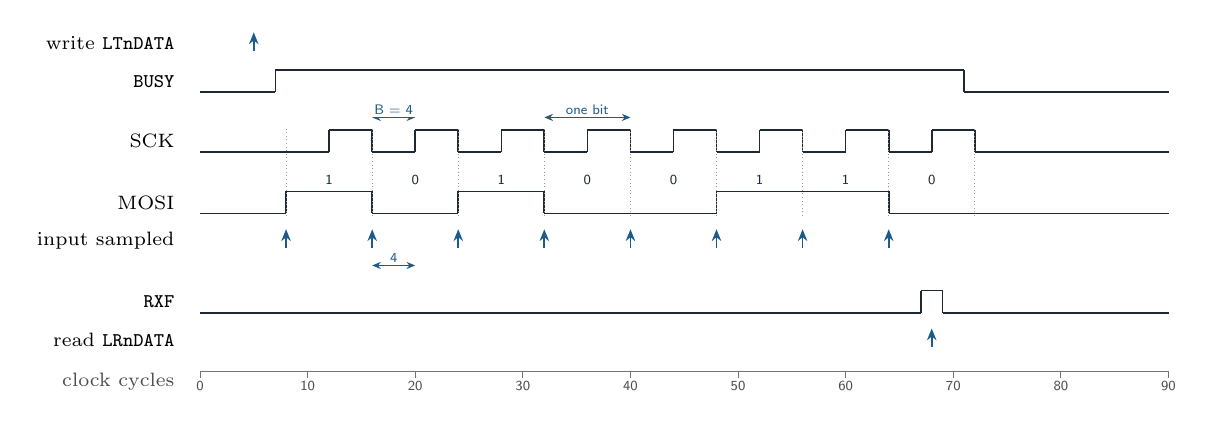
\begin{tikzpicture}[x=1mm,y=1mm]
\node[lbl,anchor=east] at (25.00,-3.40) {write \texttt{LTnDATA}};
\draw[accent,line width=0.6pt,-{Stealth[length=1.5mm,width=1.2mm]}] (33.83,-4.40) -- ++(0,2.4);
\node[lbl,anchor=east] at (25.00,-8.20) {\texttt{BUSY}};
\draw[ink,line width=0.6pt] (27.00,-9.60) -- (36.57,-9.60);
\draw[ink,line width=0.6pt] (36.57,-9.60) -- (36.57,-6.80);
\draw[ink,line width=0.6pt] (36.57,-6.80) -- (124.03,-6.80);
\draw[ink,line width=0.6pt] (124.03,-6.80) -- (124.03,-9.60);
\draw[ink,line width=0.6pt] (124.03,-9.60) -- (150.00,-9.60);
\node[lbl,anchor=east] at (25.00,-15.80) {SCK};
\draw[ink,line width=0.6pt] (27.00,-17.20) -- (43.40,-17.20);
\draw[ink,line width=0.6pt] (43.40,-17.20) -- (43.40,-14.40);
\draw[ink,line width=0.6pt] (43.40,-14.40) -- (48.87,-14.40);
\draw[ink,line width=0.6pt] (48.87,-14.40) -- (48.87,-17.20);
\draw[ink,line width=0.6pt] (48.87,-17.20) -- (54.33,-17.20);
\draw[ink,line width=0.6pt] (54.33,-17.20) -- (54.33,-14.40);
\draw[ink,line width=0.6pt] (54.33,-14.40) -- (59.80,-14.40);
\draw[ink,line width=0.6pt] (59.80,-14.40) -- (59.80,-17.20);
\draw[ink,line width=0.6pt] (59.80,-17.20) -- (65.27,-17.20);
\draw[ink,line width=0.6pt] (65.27,-17.20) -- (65.27,-14.40);
\draw[ink,line width=0.6pt] (65.27,-14.40) -- (70.73,-14.40);
\draw[ink,line width=0.6pt] (70.73,-14.40) -- (70.73,-17.20);
\draw[ink,line width=0.6pt] (70.73,-17.20) -- (76.20,-17.20);
\draw[ink,line width=0.6pt] (76.20,-17.20) -- (76.20,-14.40);
\draw[ink,line width=0.6pt] (76.20,-14.40) -- (81.67,-14.40);
\draw[ink,line width=0.6pt] (81.67,-14.40) -- (81.67,-17.20);
\draw[ink,line width=0.6pt] (81.67,-17.20) -- (87.13,-17.20);
\draw[ink,line width=0.6pt] (87.13,-17.20) -- (87.13,-14.40);
\draw[ink,line width=0.6pt] (87.13,-14.40) -- (92.60,-14.40);
\draw[ink,line width=0.6pt] (92.60,-14.40) -- (92.60,-17.20);
\draw[ink,line width=0.6pt] (92.60,-17.20) -- (98.07,-17.20);
\draw[ink,line width=0.6pt] (98.07,-17.20) -- (98.07,-14.40);
\draw[ink,line width=0.6pt] (98.07,-14.40) -- (103.53,-14.40);
\draw[ink,line width=0.6pt] (103.53,-14.40) -- (103.53,-17.20);
\draw[ink,line width=0.6pt] (103.53,-17.20) -- (109.00,-17.20);
\draw[ink,line width=0.6pt] (109.00,-17.20) -- (109.00,-14.40);
\draw[ink,line width=0.6pt] (109.00,-14.40) -- (114.47,-14.40);
\draw[ink,line width=0.6pt] (114.47,-14.40) -- (114.47,-17.20);
\draw[ink,line width=0.6pt] (114.47,-17.20) -- (119.93,-17.20);
\draw[ink,line width=0.6pt] (119.93,-17.20) -- (119.93,-14.40);
\draw[ink,line width=0.6pt] (119.93,-14.40) -- (125.40,-14.40);
\draw[ink,line width=0.6pt] (125.40,-14.40) -- (125.40,-17.20);
\draw[ink,line width=0.6pt] (125.40,-17.20) -- (150.00,-17.20);
\node[lbl,anchor=east] at (25.00,-23.60) {MOSI};
\draw[ink,line width=0.6pt] (27.00,-25.00) -- (37.93,-25.00);
\draw[ink,line width=0.6pt] (37.93,-25.00) -- (37.93,-22.20);
\draw[ink,line width=0.6pt] (37.93,-22.20) -- (48.87,-22.20);
\draw[ink,line width=0.6pt] (48.87,-22.20) -- (48.87,-25.00);
\draw[ink,line width=0.6pt] (48.87,-25.00) -- (59.80,-25.00);
\draw[ink,line width=0.6pt] (59.80,-25.00) -- (59.80,-22.20);
\draw[ink,line width=0.6pt] (59.80,-22.20) -- (70.73,-22.20);
\draw[ink,line width=0.6pt] (70.73,-22.20) -- (70.73,-25.00);
\draw[ink,line width=0.6pt] (70.73,-25.00) -- (92.60,-25.00);
\draw[ink,line width=0.6pt] (92.60,-25.00) -- (92.60,-22.20);
\draw[ink,line width=0.6pt] (92.60,-22.20) -- (114.47,-22.20);
\draw[ink,line width=0.6pt] (114.47,-22.20) -- (114.47,-25.00);
\draw[ink,line width=0.6pt] (114.47,-25.00) -- (150.00,-25.00);
\node[font=\tiny\sffamily,text=ink,inner sep=0.6pt,anchor=center] at (43.40,-20.80) {1};
\node[font=\tiny\sffamily,text=ink,inner sep=0.6pt,anchor=center] at (54.33,-20.80) {0};
\node[font=\tiny\sffamily,text=ink,inner sep=0.6pt,anchor=center] at (65.27,-20.80) {1};
\node[font=\tiny\sffamily,text=ink,inner sep=0.6pt,anchor=center] at (76.20,-20.80) {0};
\node[font=\tiny\sffamily,text=ink,inner sep=0.6pt,anchor=center] at (87.13,-20.80) {0};
\node[font=\tiny\sffamily,text=ink,inner sep=0.6pt,anchor=center] at (98.07,-20.80) {1};
\node[font=\tiny\sffamily,text=ink,inner sep=0.6pt,anchor=center] at (109.00,-20.80) {1};
\node[font=\tiny\sffamily,text=ink,inner sep=0.6pt,anchor=center] at (119.93,-20.80) {0};
\draw[black!40,line width=0.3pt,densely dotted] (37.93,-25.30) -- (37.93,-14.00);
\draw[black!40,line width=0.3pt,densely dotted] (48.87,-25.30) -- (48.87,-14.00);
\draw[black!40,line width=0.3pt,densely dotted] (59.80,-25.30) -- (59.80,-14.00);
\draw[black!40,line width=0.3pt,densely dotted] (70.73,-25.30) -- (70.73,-14.00);
\draw[black!40,line width=0.3pt,densely dotted] (81.67,-25.30) -- (81.67,-14.00);
\draw[black!40,line width=0.3pt,densely dotted] (92.60,-25.30) -- (92.60,-14.00);
\draw[black!40,line width=0.3pt,densely dotted] (103.53,-25.30) -- (103.53,-14.00);
\draw[black!40,line width=0.3pt,densely dotted] (114.47,-25.30) -- (114.47,-14.00);
\draw[black!40,line width=0.3pt,densely dotted] (125.40,-25.30) -- (125.40,-14.00);
\node[lbl,anchor=east] at (25.00,-28.40) {input sampled};
\draw[accent,line width=0.6pt,-{Stealth[length=1.5mm,width=1.2mm]}] (37.93,-29.40) -- ++(0,2.4);
\draw[accent,line width=0.6pt,-{Stealth[length=1.5mm,width=1.2mm]}] (48.87,-29.40) -- ++(0,2.4);
\draw[accent,line width=0.6pt,-{Stealth[length=1.5mm,width=1.2mm]}] (59.80,-29.40) -- ++(0,2.4);
\draw[accent,line width=0.6pt,-{Stealth[length=1.5mm,width=1.2mm]}] (70.73,-29.40) -- ++(0,2.4);
\draw[accent,line width=0.6pt,-{Stealth[length=1.5mm,width=1.2mm]}] (81.67,-29.40) -- ++(0,2.4);
\draw[accent,line width=0.6pt,-{Stealth[length=1.5mm,width=1.2mm]}] (92.60,-29.40) -- ++(0,2.4);
\draw[accent,line width=0.6pt,-{Stealth[length=1.5mm,width=1.2mm]}] (103.53,-29.40) -- ++(0,2.4);
\draw[accent,line width=0.6pt,-{Stealth[length=1.5mm,width=1.2mm]}] (114.47,-29.40) -- ++(0,2.4);
\draw[accent,line width=0.4pt,{Stealth[length=1.1mm,width=0.9mm]}-{Stealth[length=1.1mm,width=0.9mm]}] (48.87,-12.80) -- (54.33,-12.80) node[midway,above,inner sep=0.8pt,font=\tiny\sffamily,text=accent,fill=white]{B = 4};
\draw[accent,line width=0.4pt,{Stealth[length=1.1mm,width=0.9mm]}-{Stealth[length=1.1mm,width=0.9mm]}] (70.73,-12.80) -- (81.67,-12.80) node[midway,above,inner sep=0.8pt,font=\tiny\sffamily,text=accent,fill=white]{one bit};
\draw[accent,line width=0.4pt,{Stealth[length=1.1mm,width=0.9mm]}-{Stealth[length=1.1mm,width=0.9mm]}] (48.87,-31.60) -- (54.33,-31.60) node[midway,above,inner sep=0.8pt,font=\tiny\sffamily,text=accent,fill=white]{4};
\node[lbl,anchor=east] at (25.00,-36.20) {\texttt{RXF}};
\draw[ink,line width=0.6pt] (27.00,-37.60) -- (118.57,-37.60);
\draw[ink,line width=0.6pt] (118.57,-37.60) -- (118.57,-34.80);
\draw[ink,line width=0.6pt] (118.57,-34.80) -- (121.30,-34.80);
\draw[ink,line width=0.6pt] (121.30,-34.80) -- (121.30,-37.60);
\draw[ink,line width=0.6pt] (121.30,-37.60) -- (150.00,-37.60);
\node[lbl,anchor=east] at (25.00,-41.00) {read \texttt{LRnDATA}};
\draw[accent,line width=0.6pt,-{Stealth[length=1.5mm,width=1.2mm]}] (119.93,-42.00) -- ++(0,2.4);
\draw[black!55,line width=0.3pt] (27.00,-45.00) -- (150.00,-45.00);
\draw[black!55,line width=0.3pt] (27.00,-45.00) -- ++(0,-0.9) node[below,inner sep=1pt,font=\tiny\sffamily,text=black!70]{0};
\draw[black!55,line width=0.3pt] (40.67,-45.00) -- ++(0,-0.9) node[below,inner sep=1pt,font=\tiny\sffamily,text=black!70]{10};
\draw[black!55,line width=0.3pt] (54.33,-45.00) -- ++(0,-0.9) node[below,inner sep=1pt,font=\tiny\sffamily,text=black!70]{20};
\draw[black!55,line width=0.3pt] (68.00,-45.00) -- ++(0,-0.9) node[below,inner sep=1pt,font=\tiny\sffamily,text=black!70]{30};
\draw[black!55,line width=0.3pt] (81.67,-45.00) -- ++(0,-0.9) node[below,inner sep=1pt,font=\tiny\sffamily,text=black!70]{40};
\draw[black!55,line width=0.3pt] (95.33,-45.00) -- ++(0,-0.9) node[below,inner sep=1pt,font=\tiny\sffamily,text=black!70]{50};
\draw[black!55,line width=0.3pt] (109.00,-45.00) -- ++(0,-0.9) node[below,inner sep=1pt,font=\tiny\sffamily,text=black!70]{60};
\draw[black!55,line width=0.3pt] (122.67,-45.00) -- ++(0,-0.9) node[below,inner sep=1pt,font=\tiny\sffamily,text=black!70]{70};
\draw[black!55,line width=0.3pt] (136.33,-45.00) -- ++(0,-0.9) node[below,inner sep=1pt,font=\tiny\sffamily,text=black!70]{80};
\draw[black!55,line width=0.3pt] (150.00,-45.00) -- ++(0,-0.9) node[below,inner sep=1pt,font=\tiny\sffamily,text=black!70]{90};
\node[lbl,anchor=east,text=black!70] at (25.00,-46.30) {clock cycles};
\end{tikzpicture}

\caption{Example 2. The level that the receive cell takes is the one at the pin four clock cycles before the
rising clock edge. A device that answers on the falling clock edge has to deliver its data within half a bit
time minus four clock cycles: zero at B = 4, four cycles at B = 8.}
\end{figure}

\paragraph{Example 3: compare mode (pulse width, as for WS2812).} Frame \texttt{0xB0}. For WS2812 at 60\,MHz:
A = 48, B = 75, C = 24.

{\small\begin{tabularx}{\linewidth}{@{}l l L l L@{}}
\toprule
 & \multicolumn{2}{l}{Transmit cell} & \multicolumn{2}{l}{Receive cell} \\
\midrule
\texttt{LCCTRL} & \texttt{0xA0} & enabled; transmitter on &  &  \\
\texttt{LCPIN} & \texttt{0x01} & pins always driven &  &  \\
\texttt{LCOUT} & \texttt{0x10} & true output on pin 0 &  &  \\
\texttt{LCTIM} & \texttt{0x00} & next bit from the timer &  &  \\
\texttt{LCA} & \texttt{12} & high time for a one: 12 &  &  \\
\texttt{LCB} & \texttt{20} & 20 time units per bit &  &  \\
\texttt{LCC} & \texttt{5} & high time for a zero: 5 &  &  \\
\texttt{LCENC} & \texttt{0xF0} & not used &  &  \\
\texttt{LCSH} & \texttt{0xE4} & 8 bits; MSB first; compare mode &  &  \\
\texttt{LCEVM} & \texttt{0x40} & event flag on \texttt{TXE} &  &  \\
\bottomrule
\end{tabularx}
}

\begin{figure}[H]
\centering
% SPDX-FileCopyrightText: (c) 2026 Tim S. B. (GitHub: cpldcpu)
% SPDX-License-Identifier: Apache-2.0
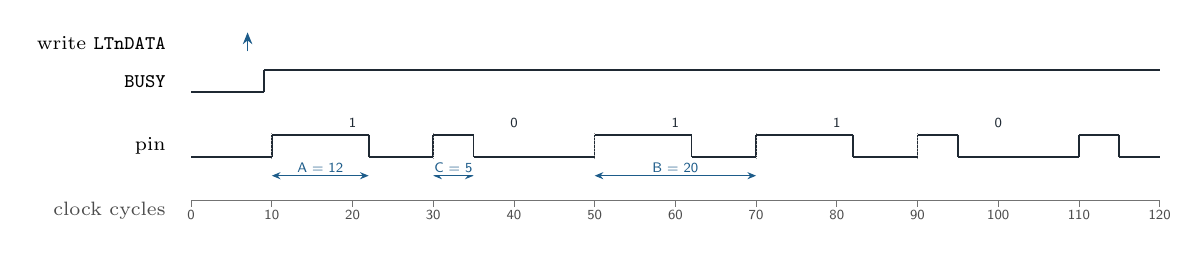
\begin{tikzpicture}[x=1mm,y=1mm]
\node[lbl,anchor=east] at (25.00,-3.40) {write \texttt{LTnDATA}};
\draw[accent,line width=0.6pt,-{Stealth[length=1.5mm,width=1.2mm]}] (34.17,-4.40) -- ++(0,2.4);
\node[lbl,anchor=east] at (25.00,-8.20) {\texttt{BUSY}};
\draw[ink,line width=0.6pt] (27.00,-9.60) -- (36.23,-9.60);
\draw[ink,line width=0.6pt] (36.23,-9.60) -- (36.23,-6.80);
\draw[ink,line width=0.6pt] (36.23,-6.80) -- (150.00,-6.80);
\node[lbl,anchor=east] at (25.00,-16.40) {pin};
\draw[ink,line width=0.6pt] (27.00,-17.80) -- (37.25,-17.80);
\draw[ink,line width=0.6pt] (37.25,-17.80) -- (37.25,-15.00);
\draw[ink,line width=0.6pt] (37.25,-15.00) -- (49.55,-15.00);
\draw[ink,line width=0.6pt] (49.55,-15.00) -- (49.55,-17.80);
\draw[ink,line width=0.6pt] (49.55,-17.80) -- (57.75,-17.80);
\draw[ink,line width=0.6pt] (57.75,-17.80) -- (57.75,-15.00);
\draw[ink,line width=0.6pt] (57.75,-15.00) -- (62.88,-15.00);
\draw[ink,line width=0.6pt] (62.88,-15.00) -- (62.88,-17.80);
\draw[ink,line width=0.6pt] (62.88,-17.80) -- (78.25,-17.80);
\draw[ink,line width=0.6pt] (78.25,-17.80) -- (78.25,-15.00);
\draw[ink,line width=0.6pt] (78.25,-15.00) -- (90.55,-15.00);
\draw[ink,line width=0.6pt] (90.55,-15.00) -- (90.55,-17.80);
\draw[ink,line width=0.6pt] (90.55,-17.80) -- (98.75,-17.80);
\draw[ink,line width=0.6pt] (98.75,-17.80) -- (98.75,-15.00);
\draw[ink,line width=0.6pt] (98.75,-15.00) -- (111.05,-15.00);
\draw[ink,line width=0.6pt] (111.05,-15.00) -- (111.05,-17.80);
\draw[ink,line width=0.6pt] (111.05,-17.80) -- (119.25,-17.80);
\draw[ink,line width=0.6pt] (119.25,-17.80) -- (119.25,-15.00);
\draw[ink,line width=0.6pt] (119.25,-15.00) -- (124.37,-15.00);
\draw[ink,line width=0.6pt] (124.37,-15.00) -- (124.37,-17.80);
\draw[ink,line width=0.6pt] (124.37,-17.80) -- (139.75,-17.80);
\draw[ink,line width=0.6pt] (139.75,-17.80) -- (139.75,-15.00);
\draw[ink,line width=0.6pt] (139.75,-15.00) -- (144.88,-15.00);
\draw[ink,line width=0.6pt] (144.88,-15.00) -- (144.88,-17.80);
\draw[ink,line width=0.6pt] (144.88,-17.80) -- (150.00,-17.80);
\node[font=\tiny\sffamily,text=ink,inner sep=0.6pt,anchor=center] at (47.50,-13.50) {1};
\draw[black!40,line width=0.3pt,densely dotted] (37.25,-18.10) -- (37.25,-14.50);
\node[font=\tiny\sffamily,text=ink,inner sep=0.6pt,anchor=center] at (68.00,-13.50) {0};
\draw[black!40,line width=0.3pt,densely dotted] (57.75,-18.10) -- (57.75,-14.50);
\node[font=\tiny\sffamily,text=ink,inner sep=0.6pt,anchor=center] at (88.50,-13.50) {1};
\draw[black!40,line width=0.3pt,densely dotted] (78.25,-18.10) -- (78.25,-14.50);
\node[font=\tiny\sffamily,text=ink,inner sep=0.6pt,anchor=center] at (109.00,-13.50) {1};
\draw[black!40,line width=0.3pt,densely dotted] (98.75,-18.10) -- (98.75,-14.50);
\node[font=\tiny\sffamily,text=ink,inner sep=0.6pt,anchor=center] at (129.50,-13.50) {0};
\draw[black!40,line width=0.3pt,densely dotted] (119.25,-18.10) -- (119.25,-14.50);
\draw[accent,line width=0.4pt,{Stealth[length=1.1mm,width=0.9mm]}-{Stealth[length=1.1mm,width=0.9mm]}] (37.25,-20.20) -- (49.55,-20.20) node[midway,above,inner sep=0.8pt,font=\tiny\sffamily,text=accent,fill=white]{A = 12};
\draw[accent,line width=0.4pt,{Stealth[length=1.1mm,width=0.9mm]}-{Stealth[length=1.1mm,width=0.9mm]}] (57.75,-20.20) -- (62.88,-20.20) node[midway,above,inner sep=0.8pt,font=\tiny\sffamily,text=accent,fill=white]{C = 5};
\draw[accent,line width=0.4pt,{Stealth[length=1.1mm,width=0.9mm]}-{Stealth[length=1.1mm,width=0.9mm]}] (78.25,-20.20) -- (98.75,-20.20) node[midway,above,inner sep=0.8pt,font=\tiny\sffamily,text=accent,fill=white]{B = 20};
\draw[black!55,line width=0.3pt] (27.00,-23.30) -- (150.00,-23.30);
\draw[black!55,line width=0.3pt] (27.00,-23.30) -- ++(0,-0.9) node[below,inner sep=1pt,font=\tiny\sffamily,text=black!70]{0};
\draw[black!55,line width=0.3pt] (37.25,-23.30) -- ++(0,-0.9) node[below,inner sep=1pt,font=\tiny\sffamily,text=black!70]{10};
\draw[black!55,line width=0.3pt] (47.50,-23.30) -- ++(0,-0.9) node[below,inner sep=1pt,font=\tiny\sffamily,text=black!70]{20};
\draw[black!55,line width=0.3pt] (57.75,-23.30) -- ++(0,-0.9) node[below,inner sep=1pt,font=\tiny\sffamily,text=black!70]{30};
\draw[black!55,line width=0.3pt] (68.00,-23.30) -- ++(0,-0.9) node[below,inner sep=1pt,font=\tiny\sffamily,text=black!70]{40};
\draw[black!55,line width=0.3pt] (78.25,-23.30) -- ++(0,-0.9) node[below,inner sep=1pt,font=\tiny\sffamily,text=black!70]{50};
\draw[black!55,line width=0.3pt] (88.50,-23.30) -- ++(0,-0.9) node[below,inner sep=1pt,font=\tiny\sffamily,text=black!70]{60};
\draw[black!55,line width=0.3pt] (98.75,-23.30) -- ++(0,-0.9) node[below,inner sep=1pt,font=\tiny\sffamily,text=black!70]{70};
\draw[black!55,line width=0.3pt] (109.00,-23.30) -- ++(0,-0.9) node[below,inner sep=1pt,font=\tiny\sffamily,text=black!70]{80};
\draw[black!55,line width=0.3pt] (119.25,-23.30) -- ++(0,-0.9) node[below,inner sep=1pt,font=\tiny\sffamily,text=black!70]{90};
\draw[black!55,line width=0.3pt] (129.50,-23.30) -- ++(0,-0.9) node[below,inner sep=1pt,font=\tiny\sffamily,text=black!70]{100};
\draw[black!55,line width=0.3pt] (139.75,-23.30) -- ++(0,-0.9) node[below,inner sep=1pt,font=\tiny\sffamily,text=black!70]{110};
\draw[black!55,line width=0.3pt] (150.00,-23.30) -- ++(0,-0.9) node[below,inner sep=1pt,font=\tiny\sffamily,text=black!70]{120};
\node[lbl,anchor=east,text=black!70] at (25.00,-24.60) {clock cycles};
\end{tikzpicture}

\caption{Example 3. Each bit lasts B = 20 cycles; the output is high for A = 12 cycles for a one and for C = 5
cycles for a zero.}
\end{figure}

\paragraph{Example 4: Manchester code (10BASE-T).} 6 clock cycles per bit. The transmit cell sends a preamble
byte, the match pattern and one data byte. The receive cell uses the time unit of half a clock cycle and takes
its timing from every bit: the edge in the middle of a bit is accepted and the sample follows three quarters of
a bit later.

{\small\begin{tabularx}{\linewidth}{@{}l l L l L@{}}
\toprule
 & \multicolumn{2}{l}{Transmit cell} & \multicolumn{2}{l}{Receive cell} \\
\midrule
\texttt{LCCTRL} & \texttt{0xA0} & enabled; transmitter on & \texttt{0xD0} & enabled; receiver on; time unit half a clock cycle \\
\texttt{LCPIN} & \texttt{0x02} & pins driven while busy & \texttt{0x10} & input pin 0; inverted \\
\texttt{LCOUT} & \texttt{0x10} & true output on pin 0 &  &  \\
\texttt{LCTIM} & \texttt{0x04} & next bit from the timer; two periods per bit & \texttt{0xE8} & both edges; accepted only while waiting; wait after each sample \\
\texttt{LCA} &  &  & \texttt{9} & 9 time units from the edge to the first sample \\
\texttt{LCB} & \texttt{3} & 3 time units per period & \texttt{24} & 24 time units between samples, and idle timeout \\
\texttt{LCDEC} &  &  & \texttt{0xF0} & level \\
\texttt{LCENC} & \texttt{0xC3} & Manchester &  &  \\
\texttt{LCSH} & \texttt{0xF0} & 8 bits; LSB first & \texttt{0xF2} & 8 bits; LSB first; search for the match pattern \\
\texttt{LCMATCH} &  &  & \texttt{0xD5} & pattern \\
\texttt{LCEVM} &  &  & \texttt{0x80} & event flag on \texttt{RXF} \\
\bottomrule
\end{tabularx}
}

\begin{figure}[H]
\centering
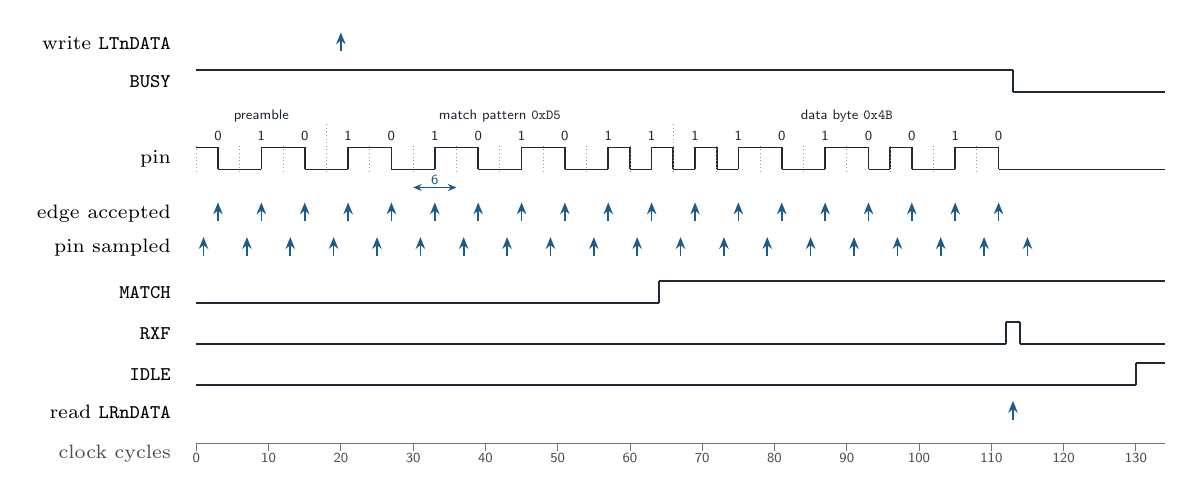
\begin{tikzpicture}[x=1mm,y=1mm]
\node[lbl,anchor=east] at (25.00,-3.40) {write \texttt{LTnDATA}};
\draw[accent,line width=0.6pt,-{Stealth[length=1.5mm,width=1.2mm]}] (45.36,-4.40) -- ++(0,2.4);
\node[lbl,anchor=east] at (25.00,-8.20) {\texttt{BUSY}};
\draw[ink,line width=0.6pt] (27.00,-6.80) -- (130.72,-6.80);
\draw[ink,line width=0.6pt] (130.72,-6.80) -- (130.72,-9.60);
\draw[ink,line width=0.6pt] (130.72,-9.60) -- (150.00,-9.60);
\node[lbl,anchor=east] at (25.00,-18.00) {pin};
\draw[ink,line width=0.6pt] (27.00,-16.60) -- (29.75,-16.60);
\draw[ink,line width=0.6pt] (29.75,-16.60) -- (29.75,-19.40);
\draw[ink,line width=0.6pt] (29.75,-19.40) -- (35.26,-19.40);
\draw[ink,line width=0.6pt] (35.26,-19.40) -- (35.26,-16.60);
\draw[ink,line width=0.6pt] (35.26,-16.60) -- (40.77,-16.60);
\draw[ink,line width=0.6pt] (40.77,-16.60) -- (40.77,-19.40);
\draw[ink,line width=0.6pt] (40.77,-19.40) -- (46.28,-19.40);
\draw[ink,line width=0.6pt] (46.28,-19.40) -- (46.28,-16.60);
\draw[ink,line width=0.6pt] (46.28,-16.60) -- (51.78,-16.60);
\draw[ink,line width=0.6pt] (51.78,-16.60) -- (51.78,-19.40);
\draw[ink,line width=0.6pt] (51.78,-19.40) -- (57.29,-19.40);
\draw[ink,line width=0.6pt] (57.29,-19.40) -- (57.29,-16.60);
\draw[ink,line width=0.6pt] (57.29,-16.60) -- (62.80,-16.60);
\draw[ink,line width=0.6pt] (62.80,-16.60) -- (62.80,-19.40);
\draw[ink,line width=0.6pt] (62.80,-19.40) -- (68.31,-19.40);
\draw[ink,line width=0.6pt] (68.31,-19.40) -- (68.31,-16.60);
\draw[ink,line width=0.6pt] (68.31,-16.60) -- (73.81,-16.60);
\draw[ink,line width=0.6pt] (73.81,-16.60) -- (73.81,-19.40);
\draw[ink,line width=0.6pt] (73.81,-19.40) -- (79.32,-19.40);
\draw[ink,line width=0.6pt] (79.32,-19.40) -- (79.32,-16.60);
\draw[ink,line width=0.6pt] (79.32,-16.60) -- (82.07,-16.60);
\draw[ink,line width=0.6pt] (82.07,-16.60) -- (82.07,-19.40);
\draw[ink,line width=0.6pt] (82.07,-19.40) -- (84.83,-19.40);
\draw[ink,line width=0.6pt] (84.83,-19.40) -- (84.83,-16.60);
\draw[ink,line width=0.6pt] (84.83,-16.60) -- (87.58,-16.60);
\draw[ink,line width=0.6pt] (87.58,-16.60) -- (87.58,-19.40);
\draw[ink,line width=0.6pt] (87.58,-19.40) -- (90.34,-19.40);
\draw[ink,line width=0.6pt] (90.34,-19.40) -- (90.34,-16.60);
\draw[ink,line width=0.6pt] (90.34,-16.60) -- (93.09,-16.60);
\draw[ink,line width=0.6pt] (93.09,-16.60) -- (93.09,-19.40);
\draw[ink,line width=0.6pt] (93.09,-19.40) -- (95.84,-19.40);
\draw[ink,line width=0.6pt] (95.84,-19.40) -- (95.84,-16.60);
\draw[ink,line width=0.6pt] (95.84,-16.60) -- (101.35,-16.60);
\draw[ink,line width=0.6pt] (101.35,-16.60) -- (101.35,-19.40);
\draw[ink,line width=0.6pt] (101.35,-19.40) -- (106.86,-19.40);
\draw[ink,line width=0.6pt] (106.86,-19.40) -- (106.86,-16.60);
\draw[ink,line width=0.6pt] (106.86,-16.60) -- (112.37,-16.60);
\draw[ink,line width=0.6pt] (112.37,-16.60) -- (112.37,-19.40);
\draw[ink,line width=0.6pt] (112.37,-19.40) -- (115.12,-19.40);
\draw[ink,line width=0.6pt] (115.12,-19.40) -- (115.12,-16.60);
\draw[ink,line width=0.6pt] (115.12,-16.60) -- (117.87,-16.60);
\draw[ink,line width=0.6pt] (117.87,-16.60) -- (117.87,-19.40);
\draw[ink,line width=0.6pt] (117.87,-19.40) -- (123.38,-19.40);
\draw[ink,line width=0.6pt] (123.38,-19.40) -- (123.38,-16.60);
\draw[ink,line width=0.6pt] (123.38,-16.60) -- (128.89,-16.60);
\draw[ink,line width=0.6pt] (128.89,-16.60) -- (128.89,-19.40);
\draw[ink,line width=0.6pt] (128.89,-19.40) -- (150.00,-19.40);
\node[font=\tiny\sffamily,text=ink,inner sep=0.6pt,anchor=center] at (29.75,-15.20) {0};
\draw[black!40,line width=0.3pt,densely dotted] (27.00,-19.70) -- (27.00,-16.10);
\node[font=\tiny\sffamily,text=ink,inner sep=0.6pt,anchor=center] at (35.26,-15.20) {1};
\draw[black!40,line width=0.3pt,densely dotted] (32.51,-19.70) -- (32.51,-16.10);
\node[font=\tiny\sffamily,text=ink,inner sep=0.6pt,anchor=center] at (40.77,-15.20) {0};
\draw[black!40,line width=0.3pt,densely dotted] (38.01,-19.70) -- (38.01,-16.10);
\node[font=\tiny\sffamily,text=ink,inner sep=0.6pt,anchor=center] at (46.28,-15.20) {1};
\draw[black!40,line width=0.3pt,densely dotted] (43.52,-19.70) -- (43.52,-13.40);
\node[font=\tiny\sffamily,text=ink,inner sep=0.6pt,anchor=center] at (51.78,-15.20) {0};
\draw[black!40,line width=0.3pt,densely dotted] (49.03,-19.70) -- (49.03,-16.10);
\node[font=\tiny\sffamily,text=ink,inner sep=0.6pt,anchor=center] at (57.29,-15.20) {1};
\draw[black!40,line width=0.3pt,densely dotted] (54.54,-19.70) -- (54.54,-16.10);
\node[font=\tiny\sffamily,text=ink,inner sep=0.6pt,anchor=center] at (62.80,-15.20) {0};
\draw[black!40,line width=0.3pt,densely dotted] (60.04,-19.70) -- (60.04,-16.10);
\node[font=\tiny\sffamily,text=ink,inner sep=0.6pt,anchor=center] at (68.31,-15.20) {1};
\draw[black!40,line width=0.3pt,densely dotted] (65.55,-19.70) -- (65.55,-16.10);
\node[font=\tiny\sffamily,text=ink,inner sep=0.6pt,anchor=center] at (73.81,-15.20) {0};
\draw[black!40,line width=0.3pt,densely dotted] (71.06,-19.70) -- (71.06,-16.10);
\node[font=\tiny\sffamily,text=ink,inner sep=0.6pt,anchor=center] at (79.32,-15.20) {1};
\draw[black!40,line width=0.3pt,densely dotted] (76.57,-19.70) -- (76.57,-16.10);
\node[font=\tiny\sffamily,text=ink,inner sep=0.6pt,anchor=center] at (84.83,-15.20) {1};
\draw[black!40,line width=0.3pt,densely dotted] (82.07,-19.70) -- (82.07,-16.10);
\node[font=\tiny\sffamily,text=ink,inner sep=0.6pt,anchor=center] at (90.34,-15.20) {1};
\draw[black!40,line width=0.3pt,densely dotted] (87.58,-19.70) -- (87.58,-13.40);
\node[font=\tiny\sffamily,text=ink,inner sep=0.6pt,anchor=center] at (95.84,-15.20) {1};
\draw[black!40,line width=0.3pt,densely dotted] (93.09,-19.70) -- (93.09,-16.10);
\node[font=\tiny\sffamily,text=ink,inner sep=0.6pt,anchor=center] at (101.35,-15.20) {0};
\draw[black!40,line width=0.3pt,densely dotted] (98.60,-19.70) -- (98.60,-16.10);
\node[font=\tiny\sffamily,text=ink,inner sep=0.6pt,anchor=center] at (106.86,-15.20) {1};
\draw[black!40,line width=0.3pt,densely dotted] (104.10,-19.70) -- (104.10,-16.10);
\node[font=\tiny\sffamily,text=ink,inner sep=0.6pt,anchor=center] at (112.37,-15.20) {0};
\draw[black!40,line width=0.3pt,densely dotted] (109.61,-19.70) -- (109.61,-16.10);
\node[font=\tiny\sffamily,text=ink,inner sep=0.6pt,anchor=center] at (117.87,-15.20) {0};
\draw[black!40,line width=0.3pt,densely dotted] (115.12,-19.70) -- (115.12,-16.10);
\node[font=\tiny\sffamily,text=ink,inner sep=0.6pt,anchor=center] at (123.38,-15.20) {1};
\draw[black!40,line width=0.3pt,densely dotted] (120.63,-19.70) -- (120.63,-16.10);
\node[font=\tiny\sffamily,text=ink,inner sep=0.6pt,anchor=center] at (128.89,-15.20) {0};
\draw[black!40,line width=0.3pt,densely dotted] (126.13,-19.70) -- (126.13,-16.10);
\node[font=\tiny\sffamily,text=ink,inner sep=0.6pt,anchor=center] at (35.26,-12.60) {preamble};
\node[font=\tiny\sffamily,text=ink,inner sep=0.6pt,anchor=center] at (65.55,-12.60) {match pattern \texttt{0xD5}};
\node[font=\tiny\sffamily,text=ink,inner sep=0.6pt,anchor=center] at (109.61,-12.60) {data byte \texttt{0x4B}};
\draw[accent,line width=0.4pt,{Stealth[length=1.1mm,width=0.9mm]}-{Stealth[length=1.1mm,width=0.9mm]}] (54.54,-21.70) -- (60.04,-21.70) node[midway,above,inner sep=0.8pt,font=\tiny\sffamily,text=accent,fill=white]{6};
\node[lbl,anchor=east] at (25.00,-25.00) {edge accepted};
\draw[accent,line width=0.6pt,-{Stealth[length=1.5mm,width=1.2mm]}] (29.75,-26.00) -- ++(0,2.4);
\draw[accent,line width=0.6pt,-{Stealth[length=1.5mm,width=1.2mm]}] (35.26,-26.00) -- ++(0,2.4);
\draw[accent,line width=0.6pt,-{Stealth[length=1.5mm,width=1.2mm]}] (40.77,-26.00) -- ++(0,2.4);
\draw[accent,line width=0.6pt,-{Stealth[length=1.5mm,width=1.2mm]}] (46.28,-26.00) -- ++(0,2.4);
\draw[accent,line width=0.6pt,-{Stealth[length=1.5mm,width=1.2mm]}] (51.78,-26.00) -- ++(0,2.4);
\draw[accent,line width=0.6pt,-{Stealth[length=1.5mm,width=1.2mm]}] (57.29,-26.00) -- ++(0,2.4);
\draw[accent,line width=0.6pt,-{Stealth[length=1.5mm,width=1.2mm]}] (62.80,-26.00) -- ++(0,2.4);
\draw[accent,line width=0.6pt,-{Stealth[length=1.5mm,width=1.2mm]}] (68.31,-26.00) -- ++(0,2.4);
\draw[accent,line width=0.6pt,-{Stealth[length=1.5mm,width=1.2mm]}] (73.81,-26.00) -- ++(0,2.4);
\draw[accent,line width=0.6pt,-{Stealth[length=1.5mm,width=1.2mm]}] (79.32,-26.00) -- ++(0,2.4);
\draw[accent,line width=0.6pt,-{Stealth[length=1.5mm,width=1.2mm]}] (84.83,-26.00) -- ++(0,2.4);
\draw[accent,line width=0.6pt,-{Stealth[length=1.5mm,width=1.2mm]}] (90.34,-26.00) -- ++(0,2.4);
\draw[accent,line width=0.6pt,-{Stealth[length=1.5mm,width=1.2mm]}] (95.84,-26.00) -- ++(0,2.4);
\draw[accent,line width=0.6pt,-{Stealth[length=1.5mm,width=1.2mm]}] (101.35,-26.00) -- ++(0,2.4);
\draw[accent,line width=0.6pt,-{Stealth[length=1.5mm,width=1.2mm]}] (106.86,-26.00) -- ++(0,2.4);
\draw[accent,line width=0.6pt,-{Stealth[length=1.5mm,width=1.2mm]}] (112.37,-26.00) -- ++(0,2.4);
\draw[accent,line width=0.6pt,-{Stealth[length=1.5mm,width=1.2mm]}] (117.87,-26.00) -- ++(0,2.4);
\draw[accent,line width=0.6pt,-{Stealth[length=1.5mm,width=1.2mm]}] (123.38,-26.00) -- ++(0,2.4);
\draw[accent,line width=0.6pt,-{Stealth[length=1.5mm,width=1.2mm]}] (128.89,-26.00) -- ++(0,2.4);
\node[lbl,anchor=east] at (25.00,-29.40) {pin sampled};
\draw[accent,line width=0.6pt,-{Stealth[length=1.5mm,width=1.2mm]}] (27.92,-30.40) -- ++(0,2.4);
\draw[accent,line width=0.6pt,-{Stealth[length=1.5mm,width=1.2mm]}] (33.43,-30.40) -- ++(0,2.4);
\draw[accent,line width=0.6pt,-{Stealth[length=1.5mm,width=1.2mm]}] (38.93,-30.40) -- ++(0,2.4);
\draw[accent,line width=0.6pt,-{Stealth[length=1.5mm,width=1.2mm]}] (44.44,-30.40) -- ++(0,2.4);
\draw[accent,line width=0.6pt,-{Stealth[length=1.5mm,width=1.2mm]}] (49.95,-30.40) -- ++(0,2.4);
\draw[accent,line width=0.6pt,-{Stealth[length=1.5mm,width=1.2mm]}] (55.46,-30.40) -- ++(0,2.4);
\draw[accent,line width=0.6pt,-{Stealth[length=1.5mm,width=1.2mm]}] (60.96,-30.40) -- ++(0,2.4);
\draw[accent,line width=0.6pt,-{Stealth[length=1.5mm,width=1.2mm]}] (66.47,-30.40) -- ++(0,2.4);
\draw[accent,line width=0.6pt,-{Stealth[length=1.5mm,width=1.2mm]}] (71.98,-30.40) -- ++(0,2.4);
\draw[accent,line width=0.6pt,-{Stealth[length=1.5mm,width=1.2mm]}] (77.49,-30.40) -- ++(0,2.4);
\draw[accent,line width=0.6pt,-{Stealth[length=1.5mm,width=1.2mm]}] (82.99,-30.40) -- ++(0,2.4);
\draw[accent,line width=0.6pt,-{Stealth[length=1.5mm,width=1.2mm]}] (88.50,-30.40) -- ++(0,2.4);
\draw[accent,line width=0.6pt,-{Stealth[length=1.5mm,width=1.2mm]}] (94.01,-30.40) -- ++(0,2.4);
\draw[accent,line width=0.6pt,-{Stealth[length=1.5mm,width=1.2mm]}] (99.51,-30.40) -- ++(0,2.4);
\draw[accent,line width=0.6pt,-{Stealth[length=1.5mm,width=1.2mm]}] (105.02,-30.40) -- ++(0,2.4);
\draw[accent,line width=0.6pt,-{Stealth[length=1.5mm,width=1.2mm]}] (110.53,-30.40) -- ++(0,2.4);
\draw[accent,line width=0.6pt,-{Stealth[length=1.5mm,width=1.2mm]}] (116.04,-30.40) -- ++(0,2.4);
\draw[accent,line width=0.6pt,-{Stealth[length=1.5mm,width=1.2mm]}] (121.54,-30.40) -- ++(0,2.4);
\draw[accent,line width=0.6pt,-{Stealth[length=1.5mm,width=1.2mm]}] (127.05,-30.40) -- ++(0,2.4);
\draw[accent,line width=0.6pt,-{Stealth[length=1.5mm,width=1.2mm]}] (132.56,-30.40) -- ++(0,2.4);
\node[lbl,anchor=east] at (25.00,-35.00) {\texttt{MATCH}};
\draw[ink,line width=0.6pt] (27.00,-36.40) -- (85.75,-36.40);
\draw[ink,line width=0.6pt] (85.75,-36.40) -- (85.75,-33.60);
\draw[ink,line width=0.6pt] (85.75,-33.60) -- (150.00,-33.60);
\node[lbl,anchor=east] at (25.00,-40.20) {\texttt{RXF}};
\draw[ink,line width=0.6pt] (27.00,-41.60) -- (129.81,-41.60);
\draw[ink,line width=0.6pt] (129.81,-41.60) -- (129.81,-38.80);
\draw[ink,line width=0.6pt] (129.81,-38.80) -- (131.64,-38.80);
\draw[ink,line width=0.6pt] (131.64,-38.80) -- (131.64,-41.60);
\draw[ink,line width=0.6pt] (131.64,-41.60) -- (150.00,-41.60);
\node[lbl,anchor=east] at (25.00,-45.40) {\texttt{IDLE}};
\draw[ink,line width=0.6pt] (27.00,-46.80) -- (146.33,-46.80);
\draw[ink,line width=0.6pt] (146.33,-46.80) -- (146.33,-44.00);
\draw[ink,line width=0.6pt] (146.33,-44.00) -- (150.00,-44.00);
\node[lbl,anchor=east] at (25.00,-50.20) {read \texttt{LRnDATA}};
\draw[accent,line width=0.6pt,-{Stealth[length=1.5mm,width=1.2mm]}] (130.72,-51.20) -- ++(0,2.4);
\draw[black!55,line width=0.3pt] (27.00,-54.20) -- (150.00,-54.20);
\draw[black!55,line width=0.3pt] (27.00,-54.20) -- ++(0,-0.9) node[below,inner sep=1pt,font=\tiny\sffamily,text=black!70]{0};
\draw[black!55,line width=0.3pt] (36.18,-54.20) -- ++(0,-0.9) node[below,inner sep=1pt,font=\tiny\sffamily,text=black!70]{10};
\draw[black!55,line width=0.3pt] (45.36,-54.20) -- ++(0,-0.9) node[below,inner sep=1pt,font=\tiny\sffamily,text=black!70]{20};
\draw[black!55,line width=0.3pt] (54.54,-54.20) -- ++(0,-0.9) node[below,inner sep=1pt,font=\tiny\sffamily,text=black!70]{30};
\draw[black!55,line width=0.3pt] (63.72,-54.20) -- ++(0,-0.9) node[below,inner sep=1pt,font=\tiny\sffamily,text=black!70]{40};
\draw[black!55,line width=0.3pt] (72.90,-54.20) -- ++(0,-0.9) node[below,inner sep=1pt,font=\tiny\sffamily,text=black!70]{50};
\draw[black!55,line width=0.3pt] (82.07,-54.20) -- ++(0,-0.9) node[below,inner sep=1pt,font=\tiny\sffamily,text=black!70]{60};
\draw[black!55,line width=0.3pt] (91.25,-54.20) -- ++(0,-0.9) node[below,inner sep=1pt,font=\tiny\sffamily,text=black!70]{70};
\draw[black!55,line width=0.3pt] (100.43,-54.20) -- ++(0,-0.9) node[below,inner sep=1pt,font=\tiny\sffamily,text=black!70]{80};
\draw[black!55,line width=0.3pt] (109.61,-54.20) -- ++(0,-0.9) node[below,inner sep=1pt,font=\tiny\sffamily,text=black!70]{90};
\draw[black!55,line width=0.3pt] (118.79,-54.20) -- ++(0,-0.9) node[below,inner sep=1pt,font=\tiny\sffamily,text=black!70]{100};
\draw[black!55,line width=0.3pt] (127.97,-54.20) -- ++(0,-0.9) node[below,inner sep=1pt,font=\tiny\sffamily,text=black!70]{110};
\draw[black!55,line width=0.3pt] (137.15,-54.20) -- ++(0,-0.9) node[below,inner sep=1pt,font=\tiny\sffamily,text=black!70]{120};
\draw[black!55,line width=0.3pt] (146.33,-54.20) -- ++(0,-0.9) node[below,inner sep=1pt,font=\tiny\sffamily,text=black!70]{130};
\node[lbl,anchor=east,text=black!70] at (25.00,-55.50) {clock cycles};
\end{tikzpicture}

\caption{Example 4, from the end of the preamble. The edges at the bit boundaries arrive while the timer runs
and are not accepted. \reg{MATCH} is set when the last eight bits equal \texttt{0xD5}; \reg{RXF} is set eight bits
later. \reg{IDLE} is set when no edge has arrived for B = 24 time units.}
\end{figure}

\paragraph{Example 5: NRZI with bit stuffing and end of packet on two outputs (USB low-speed framing).} Here at
10 clock cycles per bit; frame \texttt{0xFE}. At 60\,MHz a USB low-speed bit is 40 cycles (B = 40).

{\small% SPDX-FileCopyrightText: (c) 2026 Tim S. B. (GitHub: cpldcpu)
% SPDX-License-Identifier: Apache-2.0
\begin{tabularx}{\linewidth}{@{}l l L l L@{}}
\toprule
 & \multicolumn{2}{l}{Transmit cell} & \multicolumn{2}{l}{Receive cell} \\
\midrule
\texttt{LCCTRL} & \texttt{0xA0} & enabled; transmitter on &  &  \\
\texttt{LCPIN} & \texttt{0x02} & pins driven while busy &  &  \\
\texttt{LCOUT} & \texttt{0x13} & true output on pin 0; second output on pin 1 &  &  \\
\texttt{LCTIM} & \texttt{0x00} & next bit from the timer &  &  \\
\texttt{LCA} & \texttt{1} & not used &  &  \\
\texttt{LCB} & \texttt{10} & 10 time units per bit &  &  \\
\texttt{LCC} & \texttt{1} & not used &  &  \\
\texttt{LCENC} & \texttt{0xA5} & NRZI &  &  \\
\texttt{LCSH} & \texttt{0xF0} & 8 bits; LSB first &  &  \\
\texttt{LCRUN} & \texttt{0xC2} & insert a zero after 6 ones; both outputs low for two bit times after the last bit &  &  \\
\texttt{LCEVM} & \texttt{0x40} & event flag on \texttt{TXE} &  &  \\
\bottomrule
\end{tabularx}
}

\begin{figure}[H]
\centering
% SPDX-FileCopyrightText: (c) 2026 Tim S. B. (GitHub: cpldcpu)
% SPDX-License-Identifier: Apache-2.0
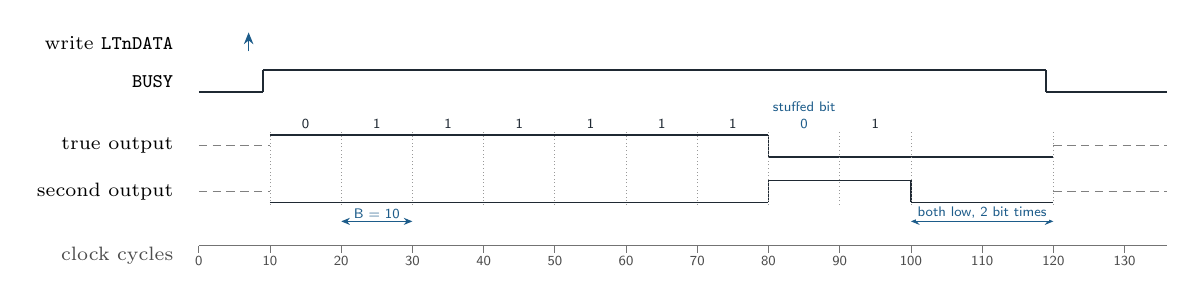
\begin{tikzpicture}[x=1mm,y=1mm]
\node[lbl,anchor=east] at (25.00,-3.40) {write \texttt{LTnDATA}};
\draw[accent,line width=0.6pt,-{Stealth[length=1.5mm,width=1.2mm]}] (33.33,-4.40) -- ++(0,2.4);
\node[lbl,anchor=east] at (25.00,-8.20) {\texttt{BUSY}};
\draw[ink,line width=0.6pt] (27.00,-9.60) -- (35.14,-9.60);
\draw[ink,line width=0.6pt] (35.14,-9.60) -- (35.14,-6.80);
\draw[ink,line width=0.6pt] (35.14,-6.80) -- (134.62,-6.80);
\draw[ink,line width=0.6pt] (134.62,-6.80) -- (134.62,-9.60);
\draw[ink,line width=0.6pt] (134.62,-9.60) -- (150.00,-9.60);
\node[lbl,anchor=east] at (25.00,-16.40) {true output};
\draw[black!50,line width=0.4pt,densely dashed] (27.00,-16.40) -- (36.04,-16.40);
\draw[ink,line width=0.6pt] (36.04,-15.00) -- (99.35,-15.00);
\draw[ink,line width=0.6pt] (99.35,-15.00) -- (99.35,-17.80);
\draw[ink,line width=0.6pt] (99.35,-17.80) -- (135.53,-17.80);
\draw[black!50,line width=0.4pt,densely dashed] (135.53,-16.40) -- (150.00,-16.40);
\node[lbl,anchor=east] at (25.00,-22.20) {second output};
\draw[black!50,line width=0.4pt,densely dashed] (27.00,-22.20) -- (36.04,-22.20);
\draw[ink,line width=0.6pt] (36.04,-23.60) -- (99.35,-23.60);
\draw[ink,line width=0.6pt] (99.35,-23.60) -- (99.35,-20.80);
\draw[ink,line width=0.6pt] (99.35,-20.80) -- (117.44,-20.80);
\draw[ink,line width=0.6pt] (117.44,-20.80) -- (117.44,-23.60);
\draw[ink,line width=0.6pt] (117.44,-23.60) -- (135.53,-23.60);
\draw[black!50,line width=0.4pt,densely dashed] (135.53,-22.20) -- (150.00,-22.20);
\node[font=\tiny\sffamily,text=ink,inner sep=0.6pt,anchor=center] at (40.57,-13.60) {0};
\draw[black!40,line width=0.3pt,densely dotted] (36.04,-23.90) -- (36.04,-14.50);
\node[font=\tiny\sffamily,text=ink,inner sep=0.6pt,anchor=center] at (49.61,-13.60) {1};
\draw[black!40,line width=0.3pt,densely dotted] (45.09,-23.90) -- (45.09,-14.50);
\node[font=\tiny\sffamily,text=ink,inner sep=0.6pt,anchor=center] at (58.65,-13.60) {1};
\draw[black!40,line width=0.3pt,densely dotted] (54.13,-23.90) -- (54.13,-14.50);
\node[font=\tiny\sffamily,text=ink,inner sep=0.6pt,anchor=center] at (67.70,-13.60) {1};
\draw[black!40,line width=0.3pt,densely dotted] (63.18,-23.90) -- (63.18,-14.50);
\node[font=\tiny\sffamily,text=ink,inner sep=0.6pt,anchor=center] at (76.74,-13.60) {1};
\draw[black!40,line width=0.3pt,densely dotted] (72.22,-23.90) -- (72.22,-14.50);
\node[font=\tiny\sffamily,text=ink,inner sep=0.6pt,anchor=center] at (85.79,-13.60) {1};
\draw[black!40,line width=0.3pt,densely dotted] (81.26,-23.90) -- (81.26,-14.50);
\node[font=\tiny\sffamily,text=ink,inner sep=0.6pt,anchor=center] at (94.83,-13.60) {1};
\draw[black!40,line width=0.3pt,densely dotted] (90.31,-23.90) -- (90.31,-14.50);
\node[font=\tiny\sffamily,text=accent,inner sep=0.6pt,anchor=center] at (103.88,-13.60) {0};
\draw[black!40,line width=0.3pt,densely dotted] (99.35,-23.90) -- (99.35,-14.50);
\node[font=\tiny\sffamily,text=ink,inner sep=0.6pt,anchor=center] at (112.92,-13.60) {1};
\draw[black!40,line width=0.3pt,densely dotted] (108.40,-23.90) -- (108.40,-14.50);
\draw[black!40,line width=0.3pt,densely dotted] (117.44,-23.90) -- (117.44,-14.50);
\draw[black!40,line width=0.3pt,densely dotted] (135.53,-23.90) -- (135.53,-14.50);
\node[font=\tiny\sffamily,text=accent,inner sep=0.6pt,anchor=center] at (103.88,-11.40) {stuffed bit};
\draw[accent,line width=0.4pt,{Stealth[length=1.1mm,width=0.9mm]}-{Stealth[length=1.1mm,width=0.9mm]}] (117.44,-26.00) -- (135.53,-26.00) node[midway,above,inner sep=0.8pt,font=\tiny\sffamily,text=accent,fill=white]{both low, 2 bit times};
\draw[accent,line width=0.4pt,{Stealth[length=1.1mm,width=0.9mm]}-{Stealth[length=1.1mm,width=0.9mm]}] (45.09,-26.00) -- (54.13,-26.00) node[midway,above,inner sep=0.8pt,font=\tiny\sffamily,text=accent,fill=white]{B = 10};
\draw[black!55,line width=0.3pt] (27.00,-29.10) -- (150.00,-29.10);
\draw[black!55,line width=0.3pt] (27.00,-29.10) -- ++(0,-0.9) node[below,inner sep=1pt,font=\tiny\sffamily,text=black!70]{0};
\draw[black!55,line width=0.3pt] (36.04,-29.10) -- ++(0,-0.9) node[below,inner sep=1pt,font=\tiny\sffamily,text=black!70]{10};
\draw[black!55,line width=0.3pt] (45.09,-29.10) -- ++(0,-0.9) node[below,inner sep=1pt,font=\tiny\sffamily,text=black!70]{20};
\draw[black!55,line width=0.3pt] (54.13,-29.10) -- ++(0,-0.9) node[below,inner sep=1pt,font=\tiny\sffamily,text=black!70]{30};
\draw[black!55,line width=0.3pt] (63.18,-29.10) -- ++(0,-0.9) node[below,inner sep=1pt,font=\tiny\sffamily,text=black!70]{40};
\draw[black!55,line width=0.3pt] (72.22,-29.10) -- ++(0,-0.9) node[below,inner sep=1pt,font=\tiny\sffamily,text=black!70]{50};
\draw[black!55,line width=0.3pt] (81.26,-29.10) -- ++(0,-0.9) node[below,inner sep=1pt,font=\tiny\sffamily,text=black!70]{60};
\draw[black!55,line width=0.3pt] (90.31,-29.10) -- ++(0,-0.9) node[below,inner sep=1pt,font=\tiny\sffamily,text=black!70]{70};
\draw[black!55,line width=0.3pt] (99.35,-29.10) -- ++(0,-0.9) node[below,inner sep=1pt,font=\tiny\sffamily,text=black!70]{80};
\draw[black!55,line width=0.3pt] (108.40,-29.10) -- ++(0,-0.9) node[below,inner sep=1pt,font=\tiny\sffamily,text=black!70]{90};
\draw[black!55,line width=0.3pt] (117.44,-29.10) -- ++(0,-0.9) node[below,inner sep=1pt,font=\tiny\sffamily,text=black!70]{100};
\draw[black!55,line width=0.3pt] (126.49,-29.10) -- ++(0,-0.9) node[below,inner sep=1pt,font=\tiny\sffamily,text=black!70]{110};
\draw[black!55,line width=0.3pt] (135.53,-29.10) -- ++(0,-0.9) node[below,inner sep=1pt,font=\tiny\sffamily,text=black!70]{120};
\draw[black!55,line width=0.3pt] (144.57,-29.10) -- ++(0,-0.9) node[below,inner sep=1pt,font=\tiny\sffamily,text=black!70]{130};
\node[lbl,anchor=east,text=black!70] at (25.00,-30.40) {clock cycles};
\end{tikzpicture}

\caption{Example 5. A zero toggles the outputs, a one keeps them. After six ones the cell inserts a zero. Then
both outputs are low for two bit times, and \reg{BUSY} stays set until then. The dashed line is the released pin.}
\end{figure}

\paragraph{Further configurations.} The table lists the settings of the other configurations that were tested:
clocked reception and transmission as SPI slave and I2C slave, WS2812 reception with forwarding, USB reception.
Timing diagrams for these are not included yet. The firmware files of the design package show their use.

\begin{table}[H]
\centering\scriptsize
\setlength{\tabcolsep}{2.5pt}
\resizebox{\textwidth}{!}{%
\begin{tabular}{@{}lccccccccccccc@{}}
\toprule
Use & CTRL & PIN & OUT & CLK & TIM & A & B & C & LUT & SH & MATCH & RUN & EVM \\
\midrule
SPI master, T & A0 & 01 & 13 & 08 & 04 & 1 & HB & 1 & enc F0 & E0 & -- & -- & -- \\
SPI master, R & C0 & 40 & -- & -- & 02 & 1 & 1 & 0 & dec F0 & E0 & -- & -- & 80 \\
SPI slave, T & A0 & 01 & 50 & 20 & 41 & 1 & 1 & 1 & enc F0 & E0 & -- & -- & -- \\
SPI slave, R & C0 & -- & -- & 30 & 41 & 1 & 1 & 0 & dec F0 & E0 & -- & -- & 80 \\
I2C slave, R & C0 & 80 & -- & B0 & 41 & 1 & 1 & 0 & dec F0 & E0 & -- & -- & 80 \\
I2C slave, T & 80 & 02 & 80 & A0 & 41 & 1 & 1 & 1 & enc F0 & E0 & -- & 04 & -- \\
WS2812 control, T & A0 & 01 & 10 & -- & -- & 48 & 75 & 24 & enc F0 & E4 & -- & -- & 40 \\
WS2812 LED, R & C0 & -- & -- & -- & 68 & 36 & 150 & 0 & dec F0 & E0 & -- & -- & 90 \\
WS2812 forward, T & 80 & 01 & 30 & -- & 02 & 48 & 70 & 24 & enc F0 & EC & -- & -- & -- \\
USB, R & C0 & $p$ & -- & $q$|01 & C0 & 20 & 40 & 0 & dec C3 & F2 & 80 & C2 & A0 \\
USB, T & A0 & 02 & $p,q$ & -- & -- & 1 & 40 & 1 & enc A5 & F0 & -- & C2 & 40 \\
\bottomrule
\end{tabular}}
\caption{Cell settings of further tested configurations, from the firmware of the design package. T: transmit cell, R: receive cell. USB values are for 60\,MHz
(40 cycles per bit); \texttt{PIN} of USB receive is the pin number in bits 7:5, \texttt{CLK} holds the pin of the
second line in bits 7:5 and \reg{BLEN} in bit 0. \texttt{OUT} of USB transmit holds both output pins with \reg{OUTEN} and \reg{NEN}.
\texttt{TIM} combines the edge rule, \reg{ACC}, \reg{STOP}, \reg{TWOPH} and \reg{TRIG} as in the bit tables of section~\ref{sec:lcregs}.}
\label{tab:cfgfw}
\end{table}

\subsection{Registers of the line cells}\label{sec:lcregs}


The four cells have the same register layout. This section describes one receive cell and one transmit cell;
the table gives the addresses of all four. A receive cell has 14 configuration registers, a transmit cell 14.
A register or field that a cell type does not have reads as zero. All configuration registers are R/W and
reset to \texttt{0x00}. Each pair has an owner core (\reg{LCOWN}); only the owner can access the cells of the pair
and sees their event flags. Configuration registers are written while the cell is disabled (\reg{EN} = 0);
while it is enabled only \reg{RXEN}, \reg{TXEN}, \reg{LOW2}, \reg{LCEVM} and \reg{LCX} may be changed. In \reg{LCX} the fields \reg{PAR}, \reg{ESTR} and \reg{BCD} keep their values while the cell is enabled.

\begin{table}[H]
\centering\small
\begin{tabular}{@{}lllll@{}}
\toprule
Cell & Configuration block & Status register & Data register & Event flag \\
\midrule
Receive cell 0 (R0) & \texttt{0x3F00} + offset & \texttt{LR0STAT} \texttt{0x08} & \texttt{LR0DATA} \texttt{0x09} & \texttt{LR0}, \reg{IFRH} bit 0 \\
Transmit cell 0 (T0) & \texttt{0x3F10} + offset & \texttt{LT0STAT} \texttt{0x0A} & \texttt{LT0DATA} \texttt{0x0B} & \texttt{LT0}, bit 1 \\
Receive cell 1 (R1) & \texttt{0x3F60} + offset & \texttt{LR1STAT} \texttt{0x10} & \texttt{LR1DATA} \texttt{0x11} & \texttt{LR1}, bit 2 \\
Transmit cell 1 (T1) & \texttt{0x3F70} + offset & \texttt{LT1STAT} \texttt{0x12} & \texttt{LT1DATA} \texttt{0x13} & \texttt{LT1}, bit 3 \\
\bottomrule
\end{tabular}
\caption{Addresses of the four line cells. R0 and T0 form pair 0, R1 and T1 pair 1. In C:
\texttt{LC\_REG(LC\_T1, LC\_ENC)} is register \texttt{LCENC} of transmit cell 1.}
\end{table}

\paragraph{Status and data.} Reading \reg{LRnDATA} returns the oldest received frame and removes it; the receive
cell holds two frames. Writing \reg{LTnDATA} stores one frame for transmission; a write while \reg{TXE} is 0 is
ignored. A status bit selected in \reg{LCEVM} sets the event flag of the cell. Latched bits are cleared by writing a
one to them. Disabling a cell clears its status and its buffers.

\begin{table}[H]
\centering\small
\begin{tabularx}{\linewidth}{@{}lllL>{\raggedright\arraybackslash}p{34mm}@{}}
\toprule
Bit & Cell & Kind & Set when & Cleared by \\
\midrule
\reg{RXF} (7) & R & level & at least one frame is in the holding register & reading \reg{LRnDATA} removes the oldest frame \\
\reg{FERR} (6) & R & latched & a frame with a wrong parity bit was received (\reg{PAR} = 1 or 2) & writing 1 \\
\reg{TXE} (6) & T & level & the frame buffer is empty; it is set again when the frame moves to the shift register & a write to \reg{LTnDATA} that is accepted \\
\reg{EOP} (5) & R & latched & both pins went low (start of both-low) & writing 1 \\
\reg{BUSY} (5) & T & level & a frame is being sent, including the end-of-packet periods & the end of the frame \\
\reg{IDLE} (4) & R & latched & the line became idle & writing 1 \\
\reg{MATCH} (3) & R & latched & the match pattern was found & writing 1 \\
\reg{OVR} (2) & R & latched & a completed frame was dropped, because the holding register was full & writing 1 \\
\reg{STUFF} (1) & R & latched & a stuffed bit broke the run-length rule & writing 1 \\
\reg{BOTHL} (0) & R & level & the input pin and the clock pin are both low, with \reg{EN} = 1 & the pins leaving the state \\
\bottomrule
\end{tabularx}
\caption{Status bits. The bits 7 and 4 to 0 of a transmit cell read as 0.}
\end{table}

\paragraph{Configuration registers.} The first column of the two tables gives the offset in the configuration block.

\begin{table}[H]
\centering\footnotesize
\setlength{\tabcolsep}{3pt}
\begin{tabular}{@{}ll|*{8}{>{\centering\arraybackslash}p{12.2mm}|}@{}}
\hline
\rowcolor{fillA}\textbf{Register} & \textbf{Addr.} & \textbf{7} & \textbf{6} & \textbf{5} & \textbf{4} & \textbf{3} & \textbf{2} & \textbf{1} & \textbf{0} \\ \hline
\texttt{LCCTRL} & \texttt{+0 R} & \texttt{EN} & \texttt{RXEN} & \textcolor{black!45}{--} & \texttt{UNIT} & \textcolor{black!45}{--} & \multicolumn{3}{c|}{\texttt{PRE}} \\ \hline
\texttt{LCPIN} & \texttt{+1 R} & \multicolumn{3}{c|}{\texttt{INSEL}} & \texttt{INV} & \multicolumn{2}{c|}{\texttt{FILT}} & \multicolumn{2}{c|}{\textcolor{black!45}{--}} \\ \hline
\texttt{LCCLK} & \texttt{+3 R} & \multicolumn{3}{c|}{\texttt{CSEL}} & \texttt{CEN} & \multicolumn{2}{c|}{\textcolor{black!45}{--}} & \texttt{CPHA} & \texttt{BLEN} \\ \hline
\texttt{LCTIM} & \texttt{+4 R} & \multicolumn{2}{c|}{\texttt{EDGE}} & \texttt{ACC} & \multicolumn{2}{c|}{\texttt{STOP}} & \texttt{TWOPH} & \multicolumn{2}{c|}{\texttt{TRIG}} \\ \hline
\texttt{LCA} & \texttt{+5 R} & \multicolumn{8}{c|}{\texttt{A}} \\ \hline
\texttt{LCB} & \texttt{+6 R} & \multicolumn{8}{c|}{\texttt{B}} \\ \hline
\texttt{LCEC} & \texttt{+7 R} & \multicolumn{4}{c|}{\textcolor{black!45}{--}} & \multicolumn{4}{c|}{\texttt{EC}} \\ \hline
\texttt{LCDEC} & \texttt{+8 R} & \multicolumn{8}{c|}{\texttt{decode table}} \\ \hline
\texttt{LCSH} & \texttt{+A R} & \multicolumn{3}{c|}{\texttt{LEN}} & \texttt{LSBF} & \multicolumn{2}{c|}{\textcolor{black!45}{--}} & \texttt{MEN} & \textcolor{black!45}{--} \\ \hline
\texttt{LCMATCH} & \texttt{+B R} & \multicolumn{8}{c|}{\texttt{pattern}} \\ \hline
\texttt{LCRUN} & \texttt{+C R} & \multicolumn{3}{c|}{\texttt{LIM}} & \texttt{RMODE} & \multicolumn{2}{c|}{\textcolor{black!45}{--}} & \multicolumn{2}{c|}{\texttt{REF}} \\ \hline
\texttt{LCEVM} & \texttt{+D R} & \multicolumn{8}{c|}{\texttt{mask over LRnSTAT}} \\ \hline
\texttt{LCCS} & \texttt{+E R} & \multicolumn{3}{c|}{\texttt{SSEL}} & \texttt{SSEN} & \texttt{SSPOL} & \multicolumn{3}{c|}{\textcolor{black!45}{--}} \\ \hline
\texttt{LCX} & \texttt{+F R} & \texttt{X9} & \texttt{ECF} & \texttt{STA} & \texttt{STP} & \texttt{BEV} & \texttt{BCD} & \multicolumn{2}{c|}{\texttt{PAR}} \\ \hline
\end{tabular}
\caption{Receive cell: bit assignment of the configuration registers.}
\end{table}

\begin{table}[H]
\centering\footnotesize
\setlength{\tabcolsep}{3pt}
\begin{tabular}{@{}ll|*{8}{>{\centering\arraybackslash}p{12.2mm}|}@{}}
\hline
\rowcolor{fillA}\textbf{Register} & \textbf{Addr.} & \textbf{7} & \textbf{6} & \textbf{5} & \textbf{4} & \textbf{3} & \textbf{2} & \textbf{1} & \textbf{0} \\ \hline
\texttt{LCCTRL} & \texttt{+0 T} & \texttt{EN} & \textcolor{black!45}{--} & \texttt{TXEN} & \multicolumn{2}{c|}{\textcolor{black!45}{--}} & \multicolumn{3}{c|}{\texttt{PRE}} \\ \hline
\texttt{LCPIN} & \texttt{+1 T} & \multicolumn{6}{c|}{\textcolor{black!45}{--}} & \multicolumn{2}{c|}{\texttt{OEM}} \\ \hline
\texttt{LCOUT} & \texttt{+2 T} & \multicolumn{3}{c|}{\texttt{OUTSEL}} & \texttt{OUTEN} & \multicolumn{3}{c|}{\texttt{NSEL}} & \texttt{NEN} \\ \hline
\texttt{LCCLK} & \texttt{+3 T} & \multicolumn{3}{c|}{\texttt{CSEL}} & \textcolor{black!45}{--} & \texttt{NFN} & \texttt{CPOL} & \texttt{CPHA} & \textcolor{black!45}{--} \\ \hline
\texttt{LCTIM} & \texttt{+4 T} & \multicolumn{2}{c|}{\texttt{EDGE}} & \multicolumn{3}{c|}{\textcolor{black!45}{--}} & \texttt{TWOPH} & \multicolumn{2}{c|}{\texttt{TRIG}} \\ \hline
\texttt{LCA} & \texttt{+5 T} & \multicolumn{8}{c|}{\texttt{A}} \\ \hline
\texttt{LCB} & \texttt{+6 T} & \multicolumn{8}{c|}{\texttt{B}} \\ \hline
\texttt{LCC} & \texttt{+7 T} & \multicolumn{8}{c|}{\texttt{C}} \\ \hline
\texttt{LCENC} & \texttt{+9 T} & \multicolumn{8}{c|}{\texttt{encode table}} \\ \hline
\texttt{LCSH} & \texttt{+A T} & \multicolumn{3}{c|}{\texttt{LEN}} & \texttt{LSBF} & \texttt{SRC} & \texttt{CMP} & \textcolor{black!45}{--} & \texttt{SS} \\ \hline
\texttt{LCRUN} & \texttt{+C T} & \multicolumn{3}{c|}{\texttt{LIM}} & \texttt{RMODE} & \texttt{LOW2} & \texttt{IDLE} & \texttt{EOP} & \textcolor{black!45}{--} \\ \hline
\texttt{LCEVM} & \texttt{+D T} & \multicolumn{8}{c|}{\texttt{mask over LTnSTAT}} \\ \hline
\texttt{LCCS} & \texttt{+E T} & \multicolumn{3}{c|}{\texttt{SSEL}} & \texttt{SSEN} & \texttt{SSPOL} & \multicolumn{3}{c|}{\textcolor{black!45}{--}} \\ \hline
\texttt{LCX} & \texttt{+F T} & \texttt{X9} & \multicolumn{4}{c|}{\textcolor{black!45}{--}} & \texttt{ESTR} & \multicolumn{2}{c|}{\texttt{PAR}} \\ \hline
\end{tabular}
\caption{Transmit cell: bit assignment of the configuration registers.}
\end{table}

\begin{table}[H]
\centering\small
\begin{tabularx}{\linewidth}{@{}llL@{}}
\toprule
Field & Bits & Meaning \\
\midrule
\reg{EN} & 1 & Cell enabled. Clearing it resets timer, bit counter, buffers and status \\
\reg{RXEN}, \reg{TXEN} & 1 + 1 & R: receiver active; while 0 the receiver is reset and the holding register keeps its frames. T: transmitter active; clearing it ends transmission at once \\
\reg{UNIT} & 1 & Time unit: peripheral clock, or both edges of the source clock (half a clock period) \\
\reg{PRE} & 3 & Prescaler for the time unit: 1, 2, 4, \dots, 128 \\
\midrule
\reg{INSEL} & 3 & Input pin, one of the eight bidirectional pins \\
\reg{INV} & 1 & Invert the input \\
\reg{FILT} & 2 & Glitch filter: off, two equal samples, majority of three \\
\reg{OEM} & 2 & Output enable: from the port direction register, always driven, driven while the cell is busy \\
\reg{OUTSEL}, \reg{OUTEN} & 3 + 1 & Pin for the true output, and its enable \\
\reg{NSEL}, \reg{NEN} & 3 + 1 & Pin for the second output, and its enable \\
\reg{NFN} & 1 & Function of the second output: complement of the true output, or bit clock \\
\reg{CSEL}, \reg{CEN} & 3 + 1 & R: separate clock pin for the edge detector, and its enable; without it the edge detector uses the input pin. T: clock pin for \reg{TRIG} = 1 \\
\reg{CPOL}, \reg{CPHA} & 1 + 1 & Idle level of the bit clock, and the clock phase: data is sampled at the first clock edge of a bit (0) or at the second (1) \\
\reg{BLEN} & 1 & Enables the both-low detector on the input pin and pin \reg{CSEL} \\
\midrule
\reg{EDGE} & 2 & Edge that is detected: none, rising, falling, both \\
\reg{ACC} & 1 & Edge accepted always, or only while the cell is waiting \\
\reg{STOP} & 2 & After expiry: keep running, stop after each sample, stop after a complete frame \\
\reg{TWOPH} & 1 & One bit takes two timer periods; the phase input of the lookup tables alternates \\
\reg{TRIG} & 2 & R: sample point from the timer, from an accepted pin edge (external clock), or from the middle of each bit of the transmit cell. T: next bit from the timer, from an edge on the clock pin, or one bit per received bit of the receive cell \\
\reg{LCA} & 8 & Loaded into the timer on an accepted edge. In compare mode: high time for a one \\
\reg{LCB} & 8 & Loaded on expiry: the bit or half-bit period. While waiting: timeout that sets \reg{IDLE} \\
\reg{LCC} & 8 & In compare mode: high time for a zero \\
\midrule
\reg{LEN} & 3 & Frame length minus one: a frame has \reg{LEN}+1 bits, 1 to 8 \\
\reg{LSBF} & 1 & Least significant bit first \\
\reg{SRC} & 1 & Bit source for transmit: own frame buffer, or the receive cell's decoded bit \\
\reg{CMP} & 1 & Transmit in compare mode (pulse width) and not through the encode table \\
\reg{MEN} & 1 & Match enabled: the bit counter resets when the shift register equals \reg{LCMATCH} \\
\reg{SS} & 1 & Transmit adds a start bit at the inverse idle level and a stop bit at the idle level \\
\reg{LIM} & 3 & Run length limit, 0 switches stuffing off \\
\reg{RMODE} & 1 & Count ones, or count equal bits \\
\reg{LOW2} & 1 & Drive both outputs low while set \\
\reg{EOP} & 1 & After the last bit of a frame both outputs are low for two bit periods; \reg{BUSY} stays set during that time. For timer-triggered transmission \\
\reg{IDLE} & 1 & Output level while not transmitting \\
\reg{REF} & 2 & Reference event for the clock loop: none, accepted edge, both pins low, both pins low after the line was idle \\
\reg{SSEL}, \reg{SSEN}, \reg{SSPOL} & 3 + 1 + 1 & Chip select pin for slave operation, its enable and its active level \\
\bottomrule
\end{tabularx}
\caption{Configuration fields.}
\label{tab:fields}
\end{table}

\begin{table}[H]
\centering\small
\begin{tabularx}{\linewidth}{@{}llL@{}}
\toprule
Field & Encoding & Values \\
\midrule
\reg{UNIT} & 1 bit & 0 peripheral clock, 1 both edges of the source clock \\
\reg{PRE} & 3 bits & Divide the time unit by $2^{\mathtt{PRE}}$ \\
\reg{FILT} & 2 bits & 0 off, 1 two equal samples, 2 majority of three, 3 reserved \\
\reg{OEM} & 2 bits & 0 from \reg{DDR}, 1 always driven, 2 driven while busy, 3 reserved \\
\reg{EDGE} & 2 bits & 0 none, 1 rising, 2 falling, 3 both. In a transmit cell with \reg{TRIG} = 1: the clock edge at which the other side samples \\
\reg{ACC} & 1 bit & 0 always, 1 only while waiting \\
\reg{STOP} & 2 bits & 0 keep running, 1 after each sample, 2 after a complete frame, 3 reserved \\
\reg{TRIG} & 2 bits & Receive cell: 0 timer started by an edge, 1 accepted pin edge, 2 middle of each bit of the transmit cell of the pair. Transmit cell: 0 timer, 1 edge on pin \reg{CSEL}, 2 one bit per received bit of the receive cell of the pair. 3 reserved \\
\reg{LEN} & 3 bits & Frame length minus one \\
\reg{PAR} & 2 bits & Additional bit after the data bits: 0 none, 1 odd parity, 2 even parity, 3 ninth data bit \reg{X9} \\
\reg{X9} & 1 bit & R, read only: additional bit of the oldest frame. T: ninth data bit of the frame that is written next \\
\reg{ESTR} & 1 bit & T with \reg{TRIG} = 1: 0 first bit at the write of the frame, 1 at the first shift edge after it \\
\reg{BCD}, \reg{BEV} & 1 bit each & R: bus condition detector on; the flags of \reg{LCX} set the event flag of the cell \\
\reg{STP}, \reg{STA}, \reg{ECF} & 1 bit each & R: stored flags for a stop condition, a start condition and the edge count; write 1 to clear; cleared while \reg{EN} = 0 \\
\reg{EC} & 4 bits & R: 0 off; 1 to 15: number of falling data edges while the clock pin is low that sets \reg{ECF} \\
\reg{SRC} & 1 bit & 0 own frame buffer, 1 decoded bit of the receive cell of the pair \\
\reg{NFN} & 1 bit & 0 complement of the true output, 1 bit clock \\
\reg{LIM} & 3 bits & Run length limit; 0 switches stuffing off \\
\reg{RMODE} & 1 bit & 0 count ones, 1 count equal bits \\
\reg{REF} & 2 bits & 0 none, 1 accepted edge, 2 both pins low, 3 both pins low after the line was idle \\
\reg{SSEL}, \reg{SSEN}, \reg{SSPOL} & 3 + 1 + 1 bits & Chip select pin, its enable and its active level. While the pin is inactive the bit counter is held in reset \\
\bottomrule
\end{tabularx}
\caption{Encoding of the line cell fields.}
\end{table}

\paragraph{Lookup tables.} The decode table is indexed by $4\cdot\mathit{pin} + 2\cdot\mathit{previous\ sample} +
\mathit{phase}$, the encode table by $4\cdot\mathit{data} + 2\cdot\mathit{phase} + \mathit{previous\ output}$.
Bit $i$ of the register is the output for index $i$.

\begin{table}[H]
\centering\small
\begin{tabular}{@{}lll@{}}
\toprule
Table & Function & Value \\
\midrule
Decode & level & \texttt{0xF0} (\texttt{LUT\_DEC\_LEVEL}) \\
Decode & inverted level & \texttt{0x0F} (\texttt{LUT\_DEC\_INVERT}) \\
Decode & NRZI, one when the level did not change & \texttt{0xC3} (\texttt{LUT\_DEC\_NRZI}) \\
Encode & NRZ & \texttt{0xF0} (\texttt{LUT\_ENC\_NRZ}) \\
Encode & NRZI, toggle on zero & \texttt{0xA5} (\texttt{LUT\_ENC\_NRZI}) \\
Encode & Manchester, first half inverted data, second half data & \texttt{0xC3} (\texttt{LUT\_ENC\_MANCH}) \\
\bottomrule
\end{tabular}
\caption{Lookup table values for common line codes.}
\end{table}


\subsection{Limits of the line cells in this revision}

\begin{itemize}
\item Frames have 1 to 8 data bits and one optional additional bit. Eight data bits with parity and two stop bits are not supported by one cell.
\item The two inputs of the bus condition detector have separate synchronisers: data that changes less than one clock cycle before or after a clock edge at the pins can be taken as a start or stop condition.
\item \reg{FERR} is one flag for the cell and is not stored with each frame.
\item The receive cell does not sample the stop bit of a start-stop frame and does not check the start bit
again after its edge. A second receive cell on the same pin can do both.
\item A transmit cell that is clocked by a pin has no underrun indication: a frame that is written late starts
in the middle of the frame time.
\item The end of packet with both outputs low is the only end sequence; the idle pulse of 10BASE-T is made by
firmware on a single-ended output.
\item Forwarding regenerates the high times of a pulse-width code and keeps the bit period of the input.
\end{itemize}

\section{16-bit timer}\label{sec:timer}

The timer counts cycles of the peripheral clock divided by $2^{\mathtt{PS}}$ while \reg{RUN} is set. It has:

\begin{itemize}
\item \textbf{Two compare values.} When the count equals \reg{OCRA} or \reg{OCRB}, the event flag \reg{OCA} or \reg{OCB}
is set. With \reg{CTC} the count restarts at zero after it has reached \reg{OCRA}, which gives a period of
\reg{OCRA}+1 counts.
\item \textbf{Overflow.} The flag \reg{OVF} is set when the count wraps from \texttt{0xFFFF} to zero.
\item \textbf{Capture.} The count is copied to \reg{ICR} and the flag \reg{CAPT} is set by an edge on a pin of the
bidirectional port, by an accepted edge of a receive cell, or by the reference event of a receive cell. This
measures pulse widths and the time of protocol events; the USB firmware uses it for the answer time.
\end{itemize}

The 16-bit registers are read low byte first and written high byte first; the header file has
\texttt{timer\_count}, \texttt{timer\_capture} and \texttt{timer\_set}. There is one timer for both cores.
Section~\ref{sec:expwm} has an example.

{\small\begin{tabularx}{\linewidth}{@{}llllL@{}}
\toprule
Address & Name & Access & Reset & Function \\
\midrule
\texttt{0x26} & \reg{TCNTL} & R/W & \texttt{0x00} & 16-bit timer count, low byte \\
\texttt{0x27} & \reg{TCNTH} & R/W & \texttt{0x00} & 16-bit timer count, high byte \\
\texttt{0x28} & \reg{ICRL} & R & \texttt{0x00} & Capture value, low byte \\
\texttt{0x29} & \reg{ICRH} & R & \texttt{0x00} & Capture value, high byte \\
\texttt{0x3F30} & \reg{TCR} & R/W & \texttt{0x00} & Run, restart at compare A, prescaler \\
\texttt{0x3F31} & \reg{TCAP} & R/W & \texttt{0x00} & Capture source and edge \\
\texttt{0x3F32} & \reg{OCRAL} & R/W & \texttt{0x00} & Compare value A, low byte \\
\texttt{0x3F33} & \reg{OCRAH} & R/W & \texttt{0x00} & Compare value A, high byte \\
\texttt{0x3F34} & \reg{OCRBL} & R/W & \texttt{0x00} & Compare value B, low byte \\
\texttt{0x3F35} & \reg{OCRBH} & R/W & \texttt{0x00} & Compare value B, high byte \\
\bottomrule
\end{tabularx}\par}

\vspace{4pt}
{\centering\footnotesize\setlength{\tabcolsep}{3pt}
\begin{tabular}{@{}ll|*{8}{>{\centering\arraybackslash}p{12.2mm}|}@{}}
\hline
\rowcolor{fillA}\textbf{Register} & \textbf{Addr.} & \textbf{7} & \textbf{6} & \textbf{5} & \textbf{4} & \textbf{3} & \textbf{2} & \textbf{1} & \textbf{0} \\ \hline
\texttt{TCR} & \texttt{0x3F30} & \texttt{RUN} & \texttt{CTC} & \multicolumn{3}{c|}{\textcolor{black!45}{--}} & \multicolumn{3}{c|}{\texttt{PS}} \\ \hline
\texttt{TCAP} & \texttt{0x3F31} & \texttt{CEDGE} & \multicolumn{2}{c|}{\texttt{CSRC}} & \multicolumn{2}{c|}{\textcolor{black!45}{--}} & \multicolumn{3}{c|}{\texttt{CPIN}} \\ \hline
\texttt{OCRAL/H} & \texttt{0x3F32/33} & \multicolumn{8}{c|}{\texttt{compare A, 16 bits}} \\ \hline
\texttt{OCRBL/H} & \texttt{0x3F34/35} & \multicolumn{8}{c|}{\texttt{compare B, 16 bits}} \\ \hline
\end{tabular}\par}

\vspace{4pt}
{\small\begin{tabularx}{\linewidth}{@{}lL@{}}
\toprule
Field & Meaning \\
\midrule
\reg{RUN}, \reg{CTC}, \reg{PS} & Timer runs; count is cleared on compare A; prescaler $2^{\mathtt{PS}}$ on the peripheral clock \\
\reg{TCAP.CSRC}, \reg{CPIN}, \reg{CEDGE} & Capture source: 0 pin \reg{CPIN} of the bidirectional port, 1 accepted edge of receive cell \reg{CPIN} (0 or 1), 2 reference event of that cell, 3 off. Edge on the pin: 0 rising, 1 falling \\
\bottomrule
\end{tabularx}\par}


\section{PWM}\label{sec:pwm}

Three PWM channels share one 8-bit counter that counts cycles of the peripheral clock divided by
$2^{\mathtt{PPS}}$ from zero to \reg{PWMTOP}. The period is \reg{PWMTOP}+1 counts. The output of channel $n$ is high
while the count is below \reg{PWMn}, so the value 0 gives a constant low level and a value above \reg{PWMTOP} a
constant high level. A new duty value is taken over when the counter restarts, so no period is cut short. An
enabled channel drives its output pin (PWM0 to PWM2) in place of the port bit. In simulation a period of 100
cycles with duty values of 25, 50 and 75 was exact while both cores ran protocols.

{\small\begin{tabularx}{\linewidth}{@{}llllL@{}}
\toprule
Address & Name & Access & Reset & Function \\
\midrule
\texttt{0x3F38} & \reg{PWMC} & R/W & \texttt{0x00} & Channel enables and prescaler \\
\texttt{0x3F39} & \reg{PWMTOP} & R/W & \texttt{0x00} & Period minus one \\
\texttt{0x3F3A} & \reg{PWM0} & R/W & \texttt{0x00} & High time of channel 0 \\
\texttt{0x3F3B} & \reg{PWM1} & R/W & \texttt{0x00} & High time of channel 1 \\
\texttt{0x3F3C} & \reg{PWM2} & R/W & \texttt{0x00} & High time of channel 2 \\
\bottomrule
\end{tabularx}\par}

\vspace{4pt}
{\centering\footnotesize\setlength{\tabcolsep}{3pt}
\begin{tabular}{@{}ll|*{8}{>{\centering\arraybackslash}p{12.2mm}|}@{}}
\hline
\rowcolor{fillA}\textbf{Register} & \textbf{Addr.} & \textbf{7} & \textbf{6} & \textbf{5} & \textbf{4} & \textbf{3} & \textbf{2} & \textbf{1} & \textbf{0} \\ \hline
\texttt{PWMC} & \texttt{0x3F38} & \textcolor{black!45}{--} & \multicolumn{3}{c|}{\texttt{PPS}} & \textcolor{black!45}{--} & \texttt{PEN2} & \texttt{PEN1} & \texttt{PEN0} \\ \hline
\texttt{PWMTOP} & \texttt{0x3F39} & \multicolumn{8}{c|}{\texttt{period minus one}} \\ \hline
\texttt{PWM0..2} & \texttt{0x3F3A-3C} & \multicolumn{8}{c|}{\texttt{duty}} \\ \hline
\end{tabular}\par}

\vspace{4pt}
{\small\begin{tabularx}{\linewidth}{@{}lL@{}}
\toprule
Field & Meaning \\
\midrule
\reg{PEN0} to \reg{PEN2}, \reg{PPS} & PWM channel enables; prescaler $2^{\mathtt{PPS}}$ on the peripheral clock \\
\bottomrule
\end{tabularx}\par}


\section{CRC unit}\label{sec:crc}

The CRC unit is a shift register of 1 to 32 bit with a programmable polynomial. It shifts towards the high or
the low bit, so it covers CRCs that are defined with either bit order. It takes its input from one of five
sources:

\begin{itemize}
\item bytes that firmware writes to \reg{CRCIN}; one byte takes four clock cycles;
\item the bits that a receive cell delivers, starting after the match pattern, without stuffed bits;
\item the bits that a transmit cell sends.
\end{itemize}

\reg{CRCVAL} can be read and written at any time; writing it sets the start value. \reg{CRCREF} holds a value
for comparison. \reg{CRCST.EQ} shows whether value and reference are equal now, \reg{CRCST.EQF} whether they were
equal at the end of the last frame. For a received packet that carries its own check sequence, the value after
the last bit is a constant (the residual) when the packet is correct, so firmware only tests \reg{EQF}:
\texttt{0xDEBB20E3} for the frame check sequence of Ethernet, \texttt{0xB001} for the CRC-16 and \texttt{0x06} for
the CRC5 of USB.

\reg{EQF} is taken from the bit stream. If the firmware lost bytes (\reg{OVR} of the receive cell), the CRC can
still be correct, so both are checked. There is one unit; a core claims it with \reg{OWNER} while the unit is
disabled, and the other core then reads zero.

\lstinputlisting{examples/ex_crc.c}

The example was compiled (385 bytes) and not simulated in this form; both uses are part of simulated firmware.

\par\vspace{5pt}\noindent\begin{minipage}{\linewidth}
\reghead{CRCIN (W) / CRCST (R)}{0x2A}{W (IN) / R (ST)}{\texttt{0x00}}
\vspace{2pt}
{\centering\footnotesize\setlength{\tabcolsep}{2pt}%
\begin{tabular}{@{}|>{\centering\arraybackslash}p{12mm}|*{8}{>{\centering\arraybackslash}p{16.9mm}|}@{}}
\hline
\rowcolor{fillD}\textbf{Bit} & \textbf{7} & \textbf{6} & \textbf{5} & \textbf{4} & \textbf{3} & \textbf{2} & \textbf{1} & \textbf{0} \\ \hline
\texttt{Write} & \multicolumn{8}{c|}{\texttt{data byte}} \\ \hline
\texttt{Read} & \texttt{EQF} & \texttt{EQ} & \texttt{BUSY} & \multicolumn{5}{c|}{\textcolor{black!45}{--}} \\ \hline
\end{tabular}\par}
\vspace{2pt}
{\small\begin{tabularx}{\linewidth}{@{}llL@{}}
\toprule
Bits & Field & Description \\
\midrule
\texttt{7:0 (W)} & \reg{CRCIN} & Write one data byte to feed the CRC unit (processes over 4 cycles); only accepted from owner core \\
\texttt{7 (R)} & \reg{EQF} & Latched equality comparison at last frame boundary (\reg{CRCVAL} == \reg{CRCREF} at last receive frame bit or last step of \reg{CRCIN}) \\
\texttt{6 (R)} & \reg{EQ} & \reg{CRCVAL} equals \reg{CRCREF} now (with left shift, compares the low \reg{CRCLEN}+1 bits) \\
\texttt{5 (R)} & \reg{BUSY} & 1 while a byte written to \reg{CRCIN} is being processed (4 clock cycles). Read only \\
\bottomrule
\end{tabularx}\par}
\end{minipage}\par

\par\vspace{5pt}\noindent\begin{minipage}{\linewidth}
\reghead{CRCCTL}{0x3F40}{R/W}{\texttt{0x00}}
\vspace{2pt}
{\centering\footnotesize\setlength{\tabcolsep}{2pt}%
\begin{tabular}{@{}|>{\centering\arraybackslash}p{12mm}|*{8}{>{\centering\arraybackslash}p{16.9mm}|}@{}}
\hline
\rowcolor{fillD}\textbf{Bit} & \textbf{7} & \textbf{6} & \textbf{5} & \textbf{4} & \textbf{3} & \textbf{2} & \textbf{1} & \textbf{0} \\ \hline
\textbf{Field} & \texttt{EN} & \texttt{RIGHT} & \multicolumn{3}{c|}{\texttt{CSRC}} & \textcolor{black!45}{--} & \texttt{BUSY} & \texttt{OWNER} \\ \hline
\end{tabular}\par}
\vspace{2pt}
{\small\begin{tabularx}{\linewidth}{@{}llL@{}}
\toprule
Bits & Field & Description \\
\midrule
\texttt{7} & \reg{EN} & CRC unit enabled \\
\texttt{6} & \reg{RIGHT} & Shift direction: 0 left (towards MSB), 1 right (towards LSB) \\
\texttt{5:3} & \reg{CSRC} & Bit source: 0 \reg{CRCIN}, 1 receive cell 0, 2 transmit cell 0, 3 receive cell 1, 4 transmit cell 1 (stuffed bits excluded) \\
\texttt{1} & \reg{BUSY} & Same busy flag as \reg{CRCST.BUSY} (1 during 4-cycle \reg{CRCIN} byte processing). Read only \\
\texttt{0} & \reg{OWNER} & Core that owns the CRC unit (0 or 1); the other core reads 0 and its writes are ignored \\
\bottomrule
\end{tabularx}\par}
\end{minipage}\par

\par\vspace{5pt}\noindent\begin{minipage}{\linewidth}
\reghead{CRCLEN}{0x3F41}{R/W}{\texttt{0x00}}
\vspace{2pt}
{\centering\footnotesize\setlength{\tabcolsep}{2pt}%
\begin{tabular}{@{}|>{\centering\arraybackslash}p{12mm}|*{8}{>{\centering\arraybackslash}p{16.9mm}|}@{}}
\hline
\rowcolor{fillD}\textbf{Bit} & \textbf{7} & \textbf{6} & \textbf{5} & \textbf{4} & \textbf{3} & \textbf{2} & \textbf{1} & \textbf{0} \\ \hline
\textbf{Field} & \multicolumn{3}{c|}{\textcolor{black!45}{--}} & \multicolumn{5}{c|}{\texttt{width minus one}} \\ \hline
\end{tabular}\par}
\vspace{2pt}
{\small\begin{tabularx}{\linewidth}{@{}llL@{}}
\toprule
Bits & Field & Description \\
\midrule
\texttt{4:0} & \reg{CRCLEN} & CRC width minus one (0 to 31, giving widths of 1 to 32 bits) \\
\bottomrule
\end{tabularx}\par}
\end{minipage}\par

\par\vspace{5pt}\noindent\begin{minipage}{\linewidth}
\reghead{CRCPOLY0..3, CRCVAL0..3, CRCREF0..3}{0x3F42--4D}{R/W}{\texttt{0x00}}
\vspace{2pt}
{\small\noindent \reg{CRCPOLY} (\texttt{0x3F42..45}): generator polynomial. \reg{CRCVAL} (\texttt{0x3F46..49}): initial/current CRC state. \reg{CRCREF} (\texttt{0x3F4A..4D}): expected residual compared against \reg{CRCVAL} for \reg{EQ}/\reg{EQF}\par}
\end{minipage}\par

\section{Host link, mailbox and debug}\label{sec:host}

\subsection{Host link}

The host link is an SPI slave on the pins HCK, HCS, HDI and HDO: mode 0, most significant bit first, chip
select active low, one command per chip select period. The pins are sampled with the system clock, so the host
clock is at most one eighth of the system clock. The host link works while the cores are in reset and needs no
firmware.

\begin{table}[H]
\centering\small
\begin{tabularx}{\linewidth}{@{}llL@{}}
\toprule
Code & Bytes after the code & Function \\
\midrule
\texttt{0x02} & address high, address low, data \ldots & Write. The address is a data address and increments in the memories. Code memory 0 is at \texttt{0x4000}, code memory 1 at \texttt{0x4800} \\
\texttt{0x03} & address high, address low, one unused byte; then data is returned & Read. In the memories the address increments; a register is read once and its value is repeated \\
\texttt{0x04} & control byte & Bit 7: core reset. Bit 4: core that the following commands refer to. Bits 1, 0: halt core 1, core 0 \\
\texttt{0x05} & one unused byte; then four bytes are returned & Status (table~\ref{tab:hstat}) \\
\texttt{0x06} & instruction, high byte first & Inject: the selected halted core executes the instruction and returns to its position \\
\texttt{0x07} & one byte & Mailbox write to the firmware; refused while the last byte has not been read \\
\texttt{0x08} & one unused byte; then mailbox status and one byte are returned & Mailbox read from the firmware \\
\texttt{0x09} & instruction, high byte first & Execute: like inject, without the return; used to set the program counter with a jump \\
\texttt{0x0A} & -- & Step: the selected core executes one instruction or one interrupt entry \\
\bottomrule
\end{tabularx}
\caption{Host link commands. Unknown codes are ignored.}
\end{table}

\begin{table}[H]
\centering\small
\begin{tabularx}{\linewidth}{@{}llL@{}}
\toprule
Byte & Bits & Meaning \\
\midrule
1 & 7 & access allowed: core reset set, or every enabled core halted and no injection running \\
 & 6 & an injection, execution or step is running \\
 & 5, 4 & break flags of core 1 and core 0 \\
 & 1, 0 & core 1, core 0 halted \\
2 & 7 & error: an access, an injection or a mailbox write was refused since the last status command \\
 & 6 & core reset \\
 & 5, 4 & core 1, core 0 waiting \\
 & 2 & selected core \\
 & 1, 0 & core 1, core 0 enabled \\
3, 4 & & program counter of the selected core, high and low byte; at the start of an instruction it is the address of that instruction plus one \\
\bottomrule
\end{tabularx}
\caption{Bytes returned by the status command.}
\label{tab:hstat}
\end{table}

\textbf{Access condition.} Memory and register access by the host is carried out only while the core reset is
set or every enabled core is halted; otherwise it is refused and the error bit is set. Halting one core for a
memory access therefore stops both. The mailbox, the status command, inject and step do not need this.

\subsection{Loading and starting a program}

After reset the core reset is set. The host writes the images to \texttt{0x4000} and \texttt{0x4800}, reads them
back if it wants to check them, and clears the core reset with the control command. Section~\ref{sec:load} shows
the sequence.

\subsection{Debugging}

The host halts a core with the control command or the firmware halts itself with \texttt{BREAK}. While a core is
halted, the host reads and writes memory and registers, reads the program counter, injects single
instructions (for instance to read a register of the core through the mailbox), and steps. Core registers are
not directly visible; they are read by injected instructions.

\subsection{Mailbox}

The mailbox passes single bytes between host and firmware while the cores run. It holds one byte in each
direction. The firmware reads a byte from the host in \reg{MBDATA} when \reg{MBSTAT.RXF} is set; the event flag
\reg{MBX} follows this bit. It writes a byte for the host to \reg{MBDATA} when \reg{MBSTAT.TXE} is set. In
simulation the host link carried one byte per 152 clock cycles with blind writes and one per 280 to 496
cycles with status polling.

\subsection{Debug pin}

The debug pin shows one internal signal selected with \reg{DBGSEL}: the sample point, the accepted edge or
the reference event of a receive cell, or the transmitted bit of a transmit cell. This makes the timing of a
line cell visible on an oscilloscope next to the line signal.

\par\vspace{5pt}\noindent\begin{minipage}{\linewidth}
\reghead{MBSTAT}{0x0C}{R}{\texttt{0x40}}
\vspace{2pt}
{\centering\footnotesize\setlength{\tabcolsep}{2pt}%
\begin{tabular}{@{}|>{\centering\arraybackslash}p{12mm}|*{8}{>{\centering\arraybackslash}p{16.9mm}|}@{}}
\hline
\rowcolor{fillD}\textbf{Bit} & \textbf{7} & \textbf{6} & \textbf{5} & \textbf{4} & \textbf{3} & \textbf{2} & \textbf{1} & \textbf{0} \\ \hline
\textbf{Field} & \texttt{RXF} & \texttt{TXE} & \multicolumn{6}{c|}{\textcolor{black!45}{--}} \\ \hline
\end{tabular}\par}
\vspace{2pt}
{\small\begin{tabularx}{\linewidth}{@{}llL@{}}
\toprule
Bits & Field & Description \\
\midrule
\texttt{7} & \reg{RXF} & 1 while an unread byte from the host is waiting in \reg{MBDATA} \\
\texttt{6} & \reg{TXE} & 1 when the outgoing mailbox is empty (host has read the last byte written by a core) \\
\bottomrule
\end{tabularx}\par}
\end{minipage}\par

\par\vspace{5pt}\noindent\begin{minipage}{\linewidth}
\reghead{MBDATA}{0x0D}{R/W}{--}
\vspace{2pt}
{\small\noindent Read: receives a byte written by the host (clears \reg{RXF}). Write: sends a byte to the host (clears \reg{TXE})\par}
\end{minipage}\par

\par\vspace{5pt}\noindent\begin{minipage}{\linewidth}
\reghead{DBGSEL}{0x3F52}{R/W}{\texttt{0x00}}
\vspace{2pt}
{\centering\footnotesize\setlength{\tabcolsep}{2pt}%
\begin{tabular}{@{}|>{\centering\arraybackslash}p{12mm}|*{8}{>{\centering\arraybackslash}p{16.9mm}|}@{}}
\hline
\rowcolor{fillD}\textbf{Bit} & \textbf{7} & \textbf{6} & \textbf{5} & \textbf{4} & \textbf{3} & \textbf{2} & \textbf{1} & \textbf{0} \\ \hline
\textbf{Field} & \texttt{EN} & \multicolumn{3}{c|}{\textcolor{black!45}{--}} & \multicolumn{4}{c|}{\texttt{SEL}} \\ \hline
\end{tabular}\par}
\vspace{2pt}
{\small\begin{tabularx}{\linewidth}{@{}llL@{}}
\toprule
Bits & Field & Description \\
\midrule
\texttt{7} & \reg{EN} & Enables routing the selected internal debug signal to pin \reg{DBG} (\texttt{uo\_out[2]}, one clock cycle latency) \\
\texttt{3:0} & \reg{SEL} & Debug signal: 0/1 sample point R0/R1, 2/3 TX bit T0/T1, 4/5 accepted edge R0/R1, 6/7 ref event R0/R1, 8/9 core 0/1 enable, 10 \texttt{bus\_hold}, 11 peripheral CKE, 12 core CKE, 13 trim measurement active, 14 valid measurement, 15 synchronised relaxation oscillator \\
\bottomrule
\end{tabularx}\par}
\end{minipage}\par

\section{Software}

\subsection{Tool chain}\label{sec:tools}

Section~\ref{sec:compiler} names the compilers and the machine option. The examples use GCC. Two linker symbols place
constants in the code memory of the core and set the size of the data memory. An image for core 1 includes
\texttt{rpe\_core1.h}, which sets its stack and start-up code, and places its variables above its stack.

\begin{lstlisting}[language=sh]
# image for core 0
avr-gcc -mmcu=attiny40 -Os -Wall -Ifw \
    -Wl,--defsym=__RODATA_PM_OFFSET__=0x4000 -Wl,--defsym=__DATA_REGION_LENGTH__=0x800 \
    -o app.elf app.c
# image for core 1
avr-gcc -mmcu=attiny40 -Os -Wall -Ifw \
    -Wl,--defsym=__RODATA_PM_OFFSET__=0x4800 -Wl,--defsym=__DATA_REGION_LENGTH__=0x800 \
    -Wl,--section-start=.data=0x800440 -o app1.elf app1.c
avr-objcopy -O binary app.elf app.bin
\end{lstlisting}

Rules for code on this core: a function gets its arguments in six registers, which is three arguments of up to 16 bit, and further arguments on the stack; protected registers are
written with \texttt{PROT\_WRITE(reg, value)}; a core waits for events with \texttt{wait\_for} and does not poll
in a loop when the other core has deadlines; large buffers are placed in the section \texttt{.noinit}.

\subsection{Loading a program from the host}\label{sec:load}

The listing shows the sequence for a host with an SPI interface. It is a sketch of the command sequence and
has not been run against the simulation in this form; the testbench contains the same sequence in Verilog.

\begin{lstlisting}[language=Python]
def cmd(*b):            # one host link command: chip select low, bytes out, bytes back
    return spi.xfer(bytes(b))

def load(image0, image1=b""):
    cmd(0x04, 0x80)                                  # core reset set, nothing halted
    for base, image in ((0x4000, image0), (0x4800, image1)):
        for i in range(0, len(image), 64):           # write command: address, then data
            a = base + i
            cmd(0x02, a >> 8, a & 0xFF, *image[i:i + 64])
    for base, image in ((0x4000, image0), (0x4800, image1)):
        back = cmd(0x03, base >> 8, base & 0xFF, 0, *([0] * len(image)))
        assert back[4:] == image                     # one unused byte follows the address
    cmd(0x04, 0x00)                                  # release the core reset: core 0 starts
\end{lstlisting}

\subsection{Example: UART echo at 115\,200 baud}

Simulated against an independent UART model at bit time errors of $-3$, 0 and $+3\,\%$; 196 bytes of code.

\lstinputlisting{examples/ex_uart_echo.c}

\subsection{Example: SPI master}

The cell settings are those of the tested SPI master firmware; the example itself was compiled (240 bytes) and
not simulated.

\lstinputlisting{examples/ex_spi_master.c}

\subsection{Example: WS2812 controller}

The cell settings are those of the tested WS2812 firmware; compiled (251 bytes), not simulated in this form.

\lstinputlisting{examples/ex_ws2812.c}

\subsection{Example: PWM and a periodic timer event}\label{sec:expwm}

Compiled (148 bytes), not simulated in this form.

\lstinputlisting{examples/ex_pwm_timer.c}

\subsection{Example: two cores with a lock and a software flag}\label{sec:ex2c}

Three files: a header with the shared variable and one image per core. The pattern is that of the tested
two-core firmware; compiled (124 and 136 bytes), not simulated in this form.

\lstinputlisting{examples/ex_shared.h}
\lstinputlisting{examples/ex_two_c0.c}
\lstinputlisting{examples/ex_two_c1.c}

\subsection{Example: I2C master read, started by an interrupt line}

Uses the tested I2C master library \texttt{i2cm.h}; compiled (816 bytes), not simulated in this form.

\lstinputlisting{examples/ex_i2c_read.c}

\subsection{Further firmware}

The design package contains complete, simulated firmware for: a USB low-speed HID device with enumeration
(\texttt{fwusb.c}, \texttt{usb\_stack.S}), a bridge from an I2C sensor to USB reports (\texttt{fwsens\_c1.c}), a
10BASE-T endpoint that answers ARP and ping (\texttt{fweth.c}), an SPI slave and an I2C slave with line cells
(\texttt{fw16\_spis.c}, \texttt{fw18\_i2cs.c}), a bridge from the host link mailbox to UART (\texttt{fwu\_mbx.c}) and
from UART to WS2812 (\texttt{fwu\_ws.c}).

\section{Application information}

\tbd: reference circuits for USB low-speed (series resistors, pull-up on D$-$), 10BASE-T (line driver,
transformer), I2C pull-ups, WS2812 level; decoupling; connection of the host link to a host controller;
layout notes.

\section{Known limitations of this revision}

\begin{itemize}
\item UART: one receive cell does not check the stop bit and does not validate the start bit. A second receive
cell on the same pin can sample the stop bit.
\item Frames have at most 8 data bits and one additional bit (parity or ninth bit).
\item Transmit cells clocked by a pin (SPI slave, I2C slave) have no underrun indication.
\item 10BASE-T: no differential idle pulse at the end of a frame and no link pulses by hardware.
\item USB from the internal oscillator needs the frame-time check of the supplied firmware.
\item A host access to memory or registers halts both cores.
\item The time base repeats after 65\,536 clock cycles (1.09\,ms at 60\,MHz).
\end{itemize}

Changes that remove the first five points are specified (specification section 18.5) and not implemented.

\section{Package and ordering information}

\tbd. The competition chip is a Tiny Tapeout design of 8x4 tiles on the IHP 130\,nm shuttle and is delivered
on the Tiny Tapeout carrier board.

\section{Revision history}

\begin{table}[H]
\centering\small
\begin{tabularx}{\linewidth}{@{}llL@{}}
\toprule
Revision & Date & Changes \\
\midrule
0.1 & 21 November 2026 & first set-up from specification draft 0.34; electrical data, package and application circuits open \\
0.2 & 21 November 2026 & table of contents; chapter order changed to memory, clocking, core, peripherals \\
0.3 & 21 November 2026 & line cells: additional frame bit (parity, ninth bit), start at the shift edge, bus condition detector and edge count; registers \reg{LCX} and \reg{LCEC}, status bit \reg{FERR} \\
\bottomrule
\end{tabularx}
\end{table}

\appendix

\section{Memory and register map}\label{sec:map}

\subsection{Memory map}

\begin{table}[H]
\centering\small
\begin{tabularx}{\linewidth}{@{}llL@{}}
\toprule
Data addresses & Size & Content \\
\midrule
\texttt{0x0000} to \texttt{0x003F} & 64 & fast I/O registers (IN, OUT; bit instructions up to \texttt{0x1F}) \\
\texttt{0x0040} to \texttt{0x083F} & 2\,048 & data memory \\
\texttt{0x0840} to \texttt{0x3EFF} & & reserved \\
\texttt{0x3F00} to \texttt{0x3FFF} & 256 & configuration page \\
\texttt{0x4000} to \texttt{0x47FF} & 2\,048 & code memory 0 \\
\texttt{0x4800} to \texttt{0x4FFF} & 2\,048 & code memory 1 \\
\bottomrule
\end{tabularx}
\caption{Data address space of both cores and of the host link.}
\end{table}

Program addresses: core 0 executes code memory 0 at word addresses 0 to 1\,023 and code memory 1 at 1\,024 to
2\,047. Core 1 executes code memory 1 at word addresses 0 to 1\,023.

\subsection{Fast I/O registers}

\begin{table}[H]
\centering\small
\begin{tabularx}{\linewidth}{@{}lllllL@{}}
\toprule
Addr. & Name & Access & Reset & Per core & Function \\
\midrule
\texttt{0x00} & \reg{PINR} & R & -- & & Bidirectional port: synchronised pin levels \\
\texttt{0x01} & \reg{DDR} & R/W & \texttt{0x00} & & Bidirectional port: direction, 1 = output \\
\texttt{0x02} & \reg{PORT} & R/W & \texttt{0x00} & & Bidirectional port: output value \\
\texttt{0x03} & \reg{PINB} & R & -- & & Input pins: synchronised levels of all eight \\
\texttt{0x04} & \reg{PORTC} & R/W & \texttt{0x00} & & Output pins \\
\texttt{0x05} & \reg{LOCK} & R/W & \texttt{0x00} & view & Four locks for mutual exclusion between the cores \\
\texttt{0x06} & \reg{IFRL} & W1C & \texttt{0x00} & bit 7 & Event flags, low byte \\
\texttt{0x07} & \reg{IFRH} & mixed & \texttt{0x00} & bits 3:0 & Event flags, high byte \\
\texttt{0x08} & \reg{LR0STAT} & mixed & \texttt{0x00} & owner & Receive cell 0: status \\
\texttt{0x09} & \reg{LR0DATA} & R & -- & owner & Receive cell 0: oldest received frame; reading removes it \\
\texttt{0x0A} & \reg{LT0STAT} & R & \texttt{0x40} & owner & Transmit cell 0: status \\
\texttt{0x0B} & \reg{LT0DATA} & W & -- & owner & Transmit cell 0: frame to transmit \\
\texttt{0x0C} & \reg{MBSTAT} & R & \texttt{0x40} & & Mailbox status \\
\texttt{0x0D} & \reg{MBDATA} & R/W & -- & & Mailbox data: read from host, write to host \\
\texttt{0x0E} & \reg{CORECTL} & R/W & \texttt{0x01} & bit 7 & Core enable, core state, number of the reading core \\
\texttt{0x0F} & \reg{CLKSTAT} & R & -- & & Clock status \\
\midrule
\texttt{0x10} & \reg{LR1STAT} & mixed & \texttt{0x00} & owner & Receive cell 1: status \\
\texttt{0x11} & \reg{LR1DATA} & R & -- & owner & Receive cell 1: oldest received frame \\
\texttt{0x12} & \reg{LT1STAT} & R & \texttt{0x40} & owner & Transmit cell 1: status \\
\texttt{0x13} & \reg{LT1DATA} & W & -- & owner & Transmit cell 1: frame to transmit \\
\texttt{0x20} & \reg{WAITL} & R/W & \texttt{0x00} & yes & Wait mask, low byte. Writing it starts the wait \\
\texttt{0x21} & \reg{WAITH} & R/W & \texttt{0x00} & yes & Wait mask, high byte \\
\texttt{0x22} & \reg{IERL} & R/W & \texttt{0x00} & yes & Interrupt enable, low byte \\
\texttt{0x23} & \reg{IERH} & R/W & \texttt{0x00} & yes & Interrupt enable, high byte \\
\texttt{0x24} & \reg{DLYL} & R/W & \texttt{0x00} & write & Read: shared time base, low byte. Write: wake-up time of the core, low byte; sets the time and clears \reg{DLY} \\
\texttt{0x25} & \reg{DLYH} & R/W & \texttt{0x00} & write & Read: time base, high byte. Write: wake-up time, high byte \\
\texttt{0x26} & \reg{TCNTL} & R/W & \texttt{0x00} & & 16-bit timer count, low byte \\
\texttt{0x27} & \reg{TCNTH} & R/W & \texttt{0x00} & & 16-bit timer count, high byte \\
\texttt{0x28} & \reg{ICRL} & R & \texttt{0x00} & & Capture value, low byte \\
\texttt{0x29} & \reg{ICRH} & R & \texttt{0x00} & & Capture value, high byte \\
\texttt{0x2A} & \reg{CRCIN}, \reg{CRCST} & R/W & \texttt{0x00} & & Write: feeds one byte to the CRC unit. Read: status of the CRC unit, bit 7 \reg{EQF}, bit 6 \reg{EQ}, bit 5 \reg{BUSY} \\
\midrule
\texttt{0x3C} & \reg{CCP} & W & -- & yes & Signature for protected writes \\
\texttt{0x3D} & \reg{SPL} & R/W & \texttt{0x00} & yes & Stack pointer, low byte \\
\texttt{0x3E} & \reg{SPH} & R/W & \texttt{0x00} & yes & Stack pointer, bits 11 to 8 \\
\texttt{0x3F} & \reg{SREG} & R/W & \texttt{0x00} & yes & Status flags \\
\bottomrule
\end{tabularx}
\caption{Fast I/O tier. Addresses \texttt{0x00} to \texttt{0x1F} are bit-addressable. Addresses not listed are reserved. 35 of 64 are used.}
\end{table}


\subsection{Configuration page}

\begin{longtable}{@{}llllp{0.47\linewidth}@{}}
\caption{Configuration page, all registers.}\\
\toprule
Address & Name & Access & Reset & Function \\
\midrule
\endfirsthead
\toprule
Address & Name & Access & Reset & Function \\
\midrule
\endhead
\bottomrule
\endfoot
\texttt{0x3F00} & \texttt{LCCTRL} & R/W & \texttt{0x00} & Receive cell 0, section~\ref{sec:lcregs} \\
\texttt{0x3F01} & \texttt{LCPIN} & R/W & \texttt{0x00} & Receive cell 0, section~\ref{sec:lcregs} \\
\texttt{0x3F03} & \texttt{LCCLK} & R/W & \texttt{0x00} & Receive cell 0, section~\ref{sec:lcregs} \\
\texttt{0x3F04} & \texttt{LCTIM} & R/W & \texttt{0x00} & Receive cell 0, section~\ref{sec:lcregs} \\
\texttt{0x3F05} & \texttt{LCA} & R/W & \texttt{0x00} & Receive cell 0, section~\ref{sec:lcregs} \\
\texttt{0x3F06} & \texttt{LCB} & R/W & \texttt{0x00} & Receive cell 0, section~\ref{sec:lcregs} \\
\texttt{0x3F07} & \texttt{LCEC} & R/W & \texttt{0x00} & Receive cell 0, section~\ref{sec:lcregs} \\
\texttt{0x3F08} & \texttt{LCDEC} & R/W & \texttt{0x00} & Receive cell 0, section~\ref{sec:lcregs} \\
\texttt{0x3F0A} & \texttt{LCSH} & R/W & \texttt{0x00} & Receive cell 0, section~\ref{sec:lcregs} \\
\texttt{0x3F0B} & \texttt{LCMATCH} & R/W & \texttt{0x00} & Receive cell 0, section~\ref{sec:lcregs} \\
\texttt{0x3F0C} & \texttt{LCRUN} & R/W & \texttt{0x00} & Receive cell 0, section~\ref{sec:lcregs} \\
\texttt{0x3F0D} & \texttt{LCEVM} & R/W & \texttt{0x00} & Receive cell 0, section~\ref{sec:lcregs} \\
\texttt{0x3F0E} & \texttt{LCCS} & R/W & \texttt{0x00} & Receive cell 0, section~\ref{sec:lcregs} \\
\texttt{0x3F0F} & \texttt{LCX} & R/W & \texttt{0x00} & Receive cell 0, section~\ref{sec:lcregs} \\
\midrule
\texttt{0x3F10} & \texttt{LCCTRL} & R/W & \texttt{0x00} & Transmit cell 0, section~\ref{sec:lcregs} \\
\texttt{0x3F11} & \texttt{LCPIN} & R/W & \texttt{0x00} & Transmit cell 0, section~\ref{sec:lcregs} \\
\texttt{0x3F12} & \texttt{LCOUT} & R/W & \texttt{0x00} & Transmit cell 0, section~\ref{sec:lcregs} \\
\texttt{0x3F13} & \texttt{LCCLK} & R/W & \texttt{0x00} & Transmit cell 0, section~\ref{sec:lcregs} \\
\texttt{0x3F14} & \texttt{LCTIM} & R/W & \texttt{0x00} & Transmit cell 0, section~\ref{sec:lcregs} \\
\texttt{0x3F15} & \texttt{LCA} & R/W & \texttt{0x00} & Transmit cell 0, section~\ref{sec:lcregs} \\
\texttt{0x3F16} & \texttt{LCB} & R/W & \texttt{0x00} & Transmit cell 0, section~\ref{sec:lcregs} \\
\texttt{0x3F17} & \texttt{LCC} & R/W & \texttt{0x00} & Transmit cell 0, section~\ref{sec:lcregs} \\
\texttt{0x3F19} & \texttt{LCENC} & R/W & \texttt{0x00} & Transmit cell 0, section~\ref{sec:lcregs} \\
\texttt{0x3F1A} & \texttt{LCSH} & R/W & \texttt{0x00} & Transmit cell 0, section~\ref{sec:lcregs} \\
\texttt{0x3F1C} & \texttt{LCRUN} & R/W & \texttt{0x00} & Transmit cell 0, section~\ref{sec:lcregs} \\
\texttt{0x3F1D} & \texttt{LCEVM} & R/W & \texttt{0x00} & Transmit cell 0, section~\ref{sec:lcregs} \\
\texttt{0x3F1E} & \texttt{LCCS} & R/W & \texttt{0x00} & Transmit cell 0, section~\ref{sec:lcregs} \\
\texttt{0x3F1F} & \texttt{LCX} & R/W & \texttt{0x00} & Transmit cell 0, section~\ref{sec:lcregs} \\
\midrule
\texttt{0x3F20} & \texttt{CLKCTL} & R/W, protected & strap & Source request, oscillator enables, loop, reference selection \\
\texttt{0x3F21} & \texttt{OSCTRIM} & R/W & \texttt{0x80} & Trim value of the oscillator \\
\texttt{0x3F22} & \texttt{CLKCDIV} & R/W, protected & \texttt{0x01} & Core clock divider minus one \\
\texttt{0x3F23} & \texttt{CLKPDIV} & R/W & \texttt{0x00} & Peripheral clock divider minus one \\
\texttt{0x3F24} & \texttt{TRINT} & R/W & \texttt{0x00} & Start of a measurement, reference periods per measurement \\
\texttt{0x3F25} & \texttt{TRCNTL} & R & \texttt{0x00} & Count of the last measurement, low byte \\
\texttt{0x3F26} & \texttt{TRCNTH} & R & \texttt{0x00} & Count of the last measurement, high byte \\
\texttt{0x3F27} & \texttt{TRTGTL} & R/W & \texttt{0x00} & Target count, low byte \\
\texttt{0x3F28} & \texttt{TRTGTH} & R/W & \texttt{0x00} & Target count, high byte \\
\texttt{0x3F29} & \texttt{TRWIN} & R/W & \texttt{0x00} & Window for a valid measurement, in units of 64 counts \\
\texttt{0x3F2A} & \texttt{CLKOUT} & R/W & \texttt{0x00} & Clock output enable and divider \\
\midrule
\texttt{0x3F30} & \texttt{TCR} & R/W & \texttt{0x00} & Run, restart at compare A, prescaler \\
\texttt{0x3F31} & \texttt{TCAP} & R/W & \texttt{0x00} & Capture source and edge \\
\texttt{0x3F32} & \texttt{OCRAL} & R/W & \texttt{0x00} & Compare value A, low byte \\
\texttt{0x3F33} & \texttt{OCRAH} & R/W & \texttt{0x00} & Compare value A, high byte \\
\texttt{0x3F34} & \texttt{OCRBL} & R/W & \texttt{0x00} & Compare value B, low byte \\
\texttt{0x3F35} & \texttt{OCRBH} & R/W & \texttt{0x00} & Compare value B, high byte \\
\midrule
\texttt{0x3F38} & \texttt{PWMC} & R/W & \texttt{0x00} & Channel enables and prescaler \\
\texttt{0x3F39} & \texttt{PWMTOP} & R/W & \texttt{0x00} & Period minus one \\
\texttt{0x3F3A} & \texttt{PWM0} & R/W & \texttt{0x00} & High time of channel 0 \\
\texttt{0x3F3B} & \texttt{PWM1} & R/W & \texttt{0x00} & High time of channel 1 \\
\texttt{0x3F3C} & \texttt{PWM2} & R/W & \texttt{0x00} & High time of channel 2 \\
\midrule
\texttt{0x3F40} & \texttt{CRCCTL} & R/W & \texttt{0x00} & Enable, shift direction, bit source, owner \\
\texttt{0x3F41} & \texttt{CRCLEN} & R/W & \texttt{0x00} & Width of the CRC minus one \\
\texttt{0x3F42--45} & \texttt{CRCPOLY0..3} & R/W & \texttt{0x00} & Polynomial, low byte first \\
\texttt{0x3F46--49} & \texttt{CRCVAL0..3} & R/W & \texttt{0x00} & CRC value, low byte first \\
\texttt{0x3F4A--4D} & \texttt{CRCREF0..3} & R/W & \texttt{0x00} & Reference value, low byte first \\
\midrule
\texttt{0x3F50} & \texttt{ARB} & R/W, protected & \texttt{0x00} & Arbiter mode \\
\texttt{0x3F51} & \texttt{LCOWN} & R/W, protected & \texttt{0x02} & Owner core of each pair of line cells \\
\texttt{0x3F52} & \texttt{DBGSEL} & R/W & \texttt{0x00} & Debug pin enable and signal selection \\
\texttt{0x3F53} & \texttt{ODE} & R/W & \texttt{0x00} & Open-drain enable per pin of the bidirectional port \\
\texttt{0x3F54} & \texttt{PCMSK} & R/W & \texttt{0x00} & Pin-change mask per pin of the bidirectional port \\
\midrule
\texttt{0x3F58} & \texttt{PMCR} & R/W, protected & \texttt{0x00} & Write enables and lock of the code memories \\
\texttt{0x3F59} & \texttt{PMLIM} & R/W, protected & \texttt{0x00} & Write-protected part of the code memories \\
\midrule
\texttt{0x3F60} & \texttt{LCCTRL} & R/W & \texttt{0x00} & Receive cell 1, section~\ref{sec:lcregs} \\
\texttt{0x3F61} & \texttt{LCPIN} & R/W & \texttt{0x00} & Receive cell 1, section~\ref{sec:lcregs} \\
\texttt{0x3F63} & \texttt{LCCLK} & R/W & \texttt{0x00} & Receive cell 1, section~\ref{sec:lcregs} \\
\texttt{0x3F64} & \texttt{LCTIM} & R/W & \texttt{0x00} & Receive cell 1, section~\ref{sec:lcregs} \\
\texttt{0x3F65} & \texttt{LCA} & R/W & \texttt{0x00} & Receive cell 1, section~\ref{sec:lcregs} \\
\texttt{0x3F66} & \texttt{LCB} & R/W & \texttt{0x00} & Receive cell 1, section~\ref{sec:lcregs} \\
\texttt{0x3F67} & \texttt{LCEC} & R/W & \texttt{0x00} & Receive cell 1, section~\ref{sec:lcregs} \\
\texttt{0x3F68} & \texttt{LCDEC} & R/W & \texttt{0x00} & Receive cell 1, section~\ref{sec:lcregs} \\
\texttt{0x3F6A} & \texttt{LCSH} & R/W & \texttt{0x00} & Receive cell 1, section~\ref{sec:lcregs} \\
\texttt{0x3F6B} & \texttt{LCMATCH} & R/W & \texttt{0x00} & Receive cell 1, section~\ref{sec:lcregs} \\
\texttt{0x3F6C} & \texttt{LCRUN} & R/W & \texttt{0x00} & Receive cell 1, section~\ref{sec:lcregs} \\
\texttt{0x3F6D} & \texttt{LCEVM} & R/W & \texttt{0x00} & Receive cell 1, section~\ref{sec:lcregs} \\
\texttt{0x3F6E} & \texttt{LCCS} & R/W & \texttt{0x00} & Receive cell 1, section~\ref{sec:lcregs} \\
\texttt{0x3F6F} & \texttt{LCX} & R/W & \texttt{0x00} & Receive cell 1, section~\ref{sec:lcregs} \\
\midrule
\texttt{0x3F70} & \texttt{LCCTRL} & R/W & \texttt{0x00} & Transmit cell 1, section~\ref{sec:lcregs} \\
\texttt{0x3F71} & \texttt{LCPIN} & R/W & \texttt{0x00} & Transmit cell 1, section~\ref{sec:lcregs} \\
\texttt{0x3F72} & \texttt{LCOUT} & R/W & \texttt{0x00} & Transmit cell 1, section~\ref{sec:lcregs} \\
\texttt{0x3F73} & \texttt{LCCLK} & R/W & \texttt{0x00} & Transmit cell 1, section~\ref{sec:lcregs} \\
\texttt{0x3F74} & \texttt{LCTIM} & R/W & \texttt{0x00} & Transmit cell 1, section~\ref{sec:lcregs} \\
\texttt{0x3F75} & \texttt{LCA} & R/W & \texttt{0x00} & Transmit cell 1, section~\ref{sec:lcregs} \\
\texttt{0x3F76} & \texttt{LCB} & R/W & \texttt{0x00} & Transmit cell 1, section~\ref{sec:lcregs} \\
\texttt{0x3F77} & \texttt{LCC} & R/W & \texttt{0x00} & Transmit cell 1, section~\ref{sec:lcregs} \\
\texttt{0x3F79} & \texttt{LCENC} & R/W & \texttt{0x00} & Transmit cell 1, section~\ref{sec:lcregs} \\
\texttt{0x3F7A} & \texttt{LCSH} & R/W & \texttt{0x00} & Transmit cell 1, section~\ref{sec:lcregs} \\
\texttt{0x3F7C} & \texttt{LCRUN} & R/W & \texttt{0x00} & Transmit cell 1, section~\ref{sec:lcregs} \\
\texttt{0x3F7D} & \texttt{LCEVM} & R/W & \texttt{0x00} & Transmit cell 1, section~\ref{sec:lcregs} \\
\texttt{0x3F7E} & \texttt{LCCS} & R/W & \texttt{0x00} & Transmit cell 1, section~\ref{sec:lcregs} \\
\texttt{0x3F7F} & \texttt{LCX} & R/W & \texttt{0x00} & Transmit cell 1, section~\ref{sec:lcregs} \\
\end{longtable}


\subsection{Bit fields of all registers}

The bit fields of the line cell registers are in section~\ref{sec:lcregs}.

\paragraph{Fast I/O registers.}

{\centering\footnotesize\setlength{\tabcolsep}{3pt}
\begin{tabular}{@{}ll|*{8}{>{\centering\arraybackslash}p{12.2mm}|}@{}}
\hline
\rowcolor{fillA}\textbf{Register} & \textbf{Addr.} & \textbf{7} & \textbf{6} & \textbf{5} & \textbf{4} & \textbf{3} & \textbf{2} & \textbf{1} & \textbf{0} \\ \hline
\texttt{LOCK} & \texttt{0x05} & \texttt{OTH3} & \texttt{OTH2} & \texttt{OTH1} & \texttt{OTH0} & \texttt{LK3} & \texttt{LK2} & \texttt{LK1} & \texttt{LK0} \\ \hline
\texttt{IFRL} & \texttt{0x06} & \texttt{DLY} & \texttt{TRIM} & \texttt{MBX} & \texttt{OVF} & \texttt{OCB} & \texttt{OCA} & \texttt{CAPT} & \texttt{PC} \\ \hline
\texttt{IFRH} & \texttt{0x07} & \texttt{SW3} & \texttt{SW2} & \texttt{SW1} & \texttt{SW0} & \texttt{LT1} & \texttt{LR1} & \texttt{LT0} & \texttt{LR0} \\ \hline
\texttt{LRnSTAT} & \texttt{0x08, 0x10} & \texttt{RXF} & \texttt{FERR} & \texttt{EOP} & \texttt{IDLE} & \texttt{MATCH} & \texttt{OVR} & \texttt{STUFF} & \texttt{BOTHL} \\ \hline
\texttt{LTnSTAT} & \texttt{0x0A, 0x12} & \textcolor{black!45}{--} & \texttt{TXE} & \texttt{BUSY} & \multicolumn{5}{c|}{\textcolor{black!45}{--}} \\ \hline
\texttt{MBSTAT} & \texttt{0x0C} & \texttt{RXF} & \texttt{TXE} & \multicolumn{6}{c|}{\textcolor{black!45}{--}} \\ \hline
\texttt{CORECTL} & \texttt{0x0E} & \texttt{ID} & \textcolor{black!45}{--} & \texttt{WAIT1} & \texttt{WAIT0} & \multicolumn{2}{c|}{\textcolor{black!45}{--}} & \texttt{EN1} & \texttt{EN0} \\ \hline
\texttt{CLKSTAT} & \texttt{0x0F} & \texttt{STRAP} & \textcolor{black!45}{--} & \texttt{MVALID} & \texttt{MDONE} & \texttt{TRIMD} & \texttt{EXTP} & \texttt{OSCRUN} & \texttt{SRC} \\ \hline
\texttt{SREG} & \texttt{0x3F} & \texttt{I} & \texttt{T} & \texttt{H} & \texttt{S} & \texttt{V} & \texttt{N} & \texttt{Z} & \texttt{C} \\ \hline
\texttt{PINB} & \texttt{0x03} & \texttt{IN7} & \texttt{IN6} & \texttt{IN5} & \texttt{REF} & \texttt{STRAP} & \texttt{HMOSI} & \texttt{HCS} & \texttt{HSCK} \\ \hline
\texttt{PORTC} & \texttt{0x04} & \texttt{OUT7} & \texttt{OUT6} & \texttt{OUT5} & \texttt{OUT4} & \texttt{OUT3} & \texttt{DBG} & \texttt{CKO} & \textcolor{black!45}{--} \\ \hline
\end{tabular}\par}

\paragraph{Configuration page} (addresses are offsets from \texttt{0x3F00}).

{\centering\footnotesize\setlength{\tabcolsep}{3pt}
\begin{tabular}{@{}ll|*{8}{>{\centering\arraybackslash}p{12.2mm}|}@{}}
\hline
\rowcolor{fillA}\textbf{Register} & \textbf{Addr.} & \textbf{7} & \textbf{6} & \textbf{5} & \textbf{4} & \textbf{3} & \textbf{2} & \textbf{1} & \textbf{0} \\ \hline
\texttt{CLKCTL} & \texttt{0x20} & \texttt{RELAXEN} & \texttt{REFCELL} & \multicolumn{2}{c|}{\texttt{REFSEL}} & \texttt{TRIMD} & \texttt{LOOP} & \texttt{OSCEN} & \texttt{SRC} \\ \hline
\texttt{OSCTRIM} & \texttt{0x21} & \multicolumn{8}{c|}{\texttt{trim value}} \\ \hline
\texttt{CLKCDIV} & \texttt{0x22} & \multicolumn{8}{c|}{\texttt{CDIV}} \\ \hline
\texttt{CLKPDIV} & \texttt{0x23} & \multicolumn{8}{c|}{\texttt{PDIV}} \\ \hline
\texttt{TRINT} & \texttt{0x24} & \texttt{MEAS} & \multicolumn{7}{c|}{\texttt{INT}} \\ \hline
\texttt{TRCNTL/H} & \texttt{0x25/26} & \multicolumn{8}{c|}{\texttt{count, 16 bits, read only}} \\ \hline
\texttt{TRTGTL/H} & \texttt{0x27/28} & \multicolumn{8}{c|}{\texttt{target, 16 bits}} \\ \hline
\texttt{TRWIN} & \texttt{0x29} & \multicolumn{8}{c|}{\texttt{window}} \\ \hline
\texttt{CLKOUT} & \texttt{0x2A} & \texttt{EN} & \multicolumn{4}{c|}{\textcolor{black!45}{--}} & \multicolumn{3}{c|}{\texttt{DIV}} \\ \hline
\texttt{TCR} & \texttt{0x30} & \texttt{RUN} & \texttt{CTC} & \multicolumn{3}{c|}{\textcolor{black!45}{--}} & \multicolumn{3}{c|}{\texttt{PS}} \\ \hline
\texttt{TCAP} & \texttt{0x31} & \texttt{CEDGE} & \multicolumn{2}{c|}{\texttt{CSRC}} & \multicolumn{2}{c|}{\textcolor{black!45}{--}} & \multicolumn{3}{c|}{\texttt{CPIN}} \\ \hline
\texttt{OCRAL/H} & \texttt{0x32/33} & \multicolumn{8}{c|}{\texttt{compare A, 16 bits}} \\ \hline
\texttt{OCRBL/H} & \texttt{0x34/35} & \multicolumn{8}{c|}{\texttt{compare B, 16 bits}} \\ \hline
\texttt{PWMC} & \texttt{0x38} & \textcolor{black!45}{--} & \multicolumn{3}{c|}{\texttt{PPS}} & \textcolor{black!45}{--} & \texttt{PEN2} & \texttt{PEN1} & \texttt{PEN0} \\ \hline
\texttt{PWMTOP} & \texttt{0x39} & \multicolumn{8}{c|}{\texttt{period minus one}} \\ \hline
\texttt{PWM0..2} & \texttt{0x3A-3C} & \multicolumn{8}{c|}{\texttt{duty}} \\ \hline
\texttt{CRCCTL} & \texttt{0x40} & \texttt{EN} & \texttt{RIGHT} & \multicolumn{3}{c|}{\texttt{CSRC}} & \textcolor{black!45}{--} & \texttt{BUSY} & \texttt{OWNER} \\ \hline
\texttt{CRCLEN} & \texttt{0x41} & \multicolumn{3}{c|}{\textcolor{black!45}{--}} & \multicolumn{5}{c|}{\texttt{width minus one}} \\ \hline
\texttt{CRCPOLY0..3} & \texttt{0x42-45} & \multicolumn{8}{c|}{\texttt{polynomial, 32 bits}} \\ \hline
\texttt{CRCVAL0..3} & \texttt{0x46-49} & \multicolumn{8}{c|}{\texttt{CRC value, 32 bits, R/W}} \\ \hline
\texttt{CRCREF0..3} & \texttt{0x4A-4D} & \multicolumn{8}{c|}{\texttt{reference value, 32 bits}} \\ \hline
\texttt{ARB} & \texttt{0x50} & \multicolumn{6}{c|}{\textcolor{black!45}{--}} & \multicolumn{2}{c|}{\texttt{MODE}} \\ \hline
\texttt{LCOWN} & \texttt{0x51} & \multicolumn{6}{c|}{\textcolor{black!45}{--}} & \texttt{OWN1} & \texttt{OWN0} \\ \hline
\texttt{DBGSEL} & \texttt{0x52} & \texttt{EN} & \multicolumn{3}{c|}{\textcolor{black!45}{--}} & \multicolumn{4}{c|}{\texttt{SEL}} \\ \hline
\texttt{ODE} & \texttt{0x53} & \multicolumn{8}{c|}{\texttt{open-drain enable per pin}} \\ \hline
\texttt{PCMSK} & \texttt{0x54} & \multicolumn{8}{c|}{\texttt{pin-change mask per pin}} \\ \hline
\texttt{PMCR} & \texttt{0x58} & \texttt{LOCK} & \multicolumn{5}{c|}{\textcolor{black!45}{--}} & \texttt{XWE} & \texttt{PWE} \\ \hline
\texttt{PMLIM} & \texttt{0x59} & \multicolumn{8}{c|}{\texttt{limit}} \\ \hline
\end{tabular}\par}


\end{document}
